% !TeX root = ../../book.tex

\chapter[关系与模算术]{关系与模算术:构造集合与整数性质的证明}\label{ch:chapter06}

% !TeX root = ../../../book.tex
\section{引言}

在奠定了必要的数学术语和概念基础之后,很自然地想知道接下来的方向!正如我们之前严格定义了数学归纳法,在接下来的两章中,我们将进一步探讨一个你可能已有直观理解但尚未精确定义的概念:\textbf{函数}。

为此,我们将从\textbf{关系}这一基本概念入手,进而讨论\textbf{等价关系}——这对研究集合的性质至关重要。特别地,我们将利用整数集 $\mathbb{Z}$ 上的等价关系来阐述并证明诸多有趣的整数性质。这将带我们初窥\textbf{数论}这一丰富领域。通过陈述并证明关键定理,再运用这些定理解决具体问题,我们将开启对初等数论的探索。此后,我们将回归核心目标,在下一章继续深入探讨函数的概念。

% !TeX root = ../../../book.tex

\subsection{目标}

以下内容简要说明本章在本书中的定位。我们将解释前期工作如何为本章研究奠定基础,阐明探讨本章主题的动机,并概述学习目标及注意事项。我们会先总结本章的主要目标,概括你在学完本章后应掌握的技能与知识。后续章节将详细展开这些思想,此处仅提供一个简要列表作为学习指引。完成本章后,请你返回此列表,确认自己是否达成了所有目标。你是否能理解这些目标的重要性?能否清晰地解释相关术语并熟练地应用相关技术?

\textbf{学完本章后,你应该能够……}

\begin{itemize}
    \item 定义关系并给出多个例子。
    \item 定义并理解关系的各种属性,举例说明哪些关系具备或不具备这些属性。
    \item 研究已定义的关系,发现并证明其属性。
    \item 定义等价关系和等价类,并解释其重要性与意义。
    \item 研究已定义的等价关系,并对等价类进行分类。
    \item 利用整数集上的特定等价关系,陈述并证明数论中的有趣结论。
    \item 定义乘法逆元的概念,理解其在模算术中的意义,并应用此概念证明或证伪特定方程的解。
    \item 陈述并理解数论中的各种定理,应用这些定理解决问题。
\end{itemize}

% !TeX root = ../../../book.tex

\subsection{承上}

本章内容不像之前章节那样紧密关联,而是开启了本书的\emph{新篇章}。从现在起,我们将运用先前学到的所有数学知识探索新领域。此前的学习都是为此刻做准备:我们将提出复杂命题并用证明技巧加以论证,提供定义和定理,并期望你用这些工具证明其他命题。可以说,本章是对之前\emph{所有}章节的综合应用,我们将充分利用之前积累的知识、术语和经验!

% !TeX root = ../../../book.tex

\subsection{启下}

你可能在微积分中处理过函数(如微分与积分),在高中代数课上绘制过函数图像或求根,甚至在计算机科学中编写过递归算法。但尝试\emph{定义}函数本身是另一码事——如何向从未接触数学的人解释?如何向超智能外星人说明?若以数学归纳法般的严谨性表述,该怎么做?这并非易事。

为了深入理解\emph{函数}概念,我们需要先探讨\emph{关系}——一种比较集合元素的方法。通过大量例子了解其性质后,下一章将揭示函数本质是关系的特殊类型!讨论过程中,我们将探究关系属性,发现特定属性组合形成的重要性质。尤其将看到\emph{等价关系}自然生成集合\emph{划分},反之亦然。这一洞见将助力我们陈述并证明关于整数的关键结论。

% !TeX root = ../../../book.tex

\subsection{忠告}

本章将继续探讨抽象概念和严谨的数学内容,因此,如果你对这些日益抽象的内容和相关语言感到不适,千万不要因此就认为这些信息``无关紧要''或``百无一用''。这些概念会贯穿整本书,甚至整个数学领域!所以,当你感觉难以集中注意力时,请记住这一点。我们建议你记下学习笔记,以便提醒自己当前的学习内容。当你看到一个定理并多次阅读后终于理解时,可以在书的边缘写下定理的摘要,方便以后查阅。画一些小图形帮助你理解例子或定理的重要部分。遇到定义时,写下一个典型例子和一个反例。读完证明后,记下论证步骤的大纲,这样可以将概念``模块化'',便于更有效地记忆和回忆。如果你对某个定义、定理或证明感到困惑,也要记下来!带着问题去问同学、朋友、助教或教授,看看他们能否帮你解答。最重要的是,请记住,理解消化和融会贯通这些抽象概念和论证需要\emph{时间},通过例子验证自己是否跟上进度依然非常重要。如果你能理解并向别人解释某个概念,那说明你已经掌握得很好了。

\newpage
% !TeX root = ../../book.tex
\section{抽象(二元)关系}

% !TeX root = ../../../book.tex

\subsection{定义}

让我们直入主题,开始讨论关系。我们会先给出定义,然后提供一系列例子。

\begin{definition}
    设 $A, B$ 为集合。$A$ 和 $B$ 之间的\dotuline{关系}是由\dotuline{有序对}组成的集合,$R \subseteq A \times B$。对于元素 $a \in A$ 和 $b \in B$,当且仅当 $(a, b) \in R$ 时,我们说 $a$ 和 $b$ 是\dotuline{相关的}。

    集合 $A$ 称为\dotuline{定义域},集合 $B$ 称为\dotuline{值域}。集合 $R$ 称为\dotuline{关系集}。
    
    如果 $A = B$,我们称 $R$ 为 $A$ 上的关系。
\end{definition}

另一种常见的写法是用 $x \;R\; y$ 来表示 $(x,y) \in R$。当我们通过这种方式定义关系时,会坚持使用 $(x, y) \in R$ 来表示其基础集合结构。之后,我们有时会用一些符号来定义关系,比如 $x < y$ 或 $x \;\bigstar\; y$ 等等。

\begin{remark}
    我们这里定义的关系有时也叫\emph{二元关系},因为它涉及两个``输入'';集合 $R$ 是由\emph{有序对}组成的。

    我们可以将这个概念推广到\emph{三元关系}。也就是说,给定集合 $A,B,C$,我们可以定义 $R \subseteq A \times B \times C$ 为三元关系,当且仅当 $(a, b, c) \in R$ 时,$a,b,c$ 是相关的。我们还可以进一步推广到具有 $n$ 个``输入''的关系。不过,在本书中,我们只考虑\emph{二元关系},因此``\emph{关系}''一词将专指\emph{二元关系}。
\end{remark}

\begin{remark}
    关系 $R$ 通常通过确定 $A$ 和 $B$ 元素的某个\emph{性质}来定义(用变量命题 $P(a,b)$ 表示),并设定
    \[(a,b) \in R \iff P(a,b)\]
\end{remark}

\subsubsection*{示例}

\begin{example}
    设 $W=\{\text{英文单词}\}, L=\{\text{英文字母}\}$,定义关系 $R$ 如下:
    \[(w, \ell) \in R \iff w \text{以 } \ell \text{ 开头}\]
    则 $(\text{mathematics},\text{m}) \in R$ 且 $(\text{golf},\text{g}) \in R$,因为这些都是有效的单词,我们已经确定了它们的首字母。再来看一些反例,比如 $(\text{knowledge},\text{n}) \notin R$ 且 $(\text{you},\text{u}) \notin R$。此外 $(\text{zyzyxyqy},\text{z}) \notin R$,因为 $\text{zyzyxyqy} \notin W$。
\end{example}

$A = B$ 的情况经常出现,所以 $R$ 定义了同一集合中元素对之间的关系。下一个例子就是针对这种情况的。\\

\begin{example} \label{ex:example6.2.5}
    设 $A=B=\mathbb{Z}$,定义 $\mathbb{Z}$ 上的关系 $R$ 如下:
    \[(x, y) \in R \iff x \text{ 和 } y \text{ 具有相同的奇偶性}\]
    则 $(2,8) \in R, (-3, 7) \in R, (-99, -99) \in R$,但 $(1,2) \notin R, (0, -3) \notin R$,且 $(\pi, 0) \notin R$(因为 $\pi \notin \mathbb{Z}$)。
\end{example}

\begin{example} \label{ex:example6.2.6}
    定义 $\mathbb{R}$ 上的关系 $L$ 如下:
    \[(x, y) \in L \iff x < y\]
    则 $(-1, \pi) \in L$ 且 $(0, 100) \in L$,但 $(2, 2) \notin L$ 且 $(\pi, -1) \notin L$。
\end{example}

请注意,这里的对都是\emph{有序对}(我们可能会忘记这一点,因为 $A = B = \mathbb{R}$),所以元素的顺序很重要。确实,知道 $(x, y) \in L$ 并不一定意味着 $(y, x) \in L$。在上面这个例子中,这种情况实际上总是错误的!

回想一下,我们有时用 $x \;L\; y$ 来表示 $(x, y) \in L$,所以我们可以说 $-1 \;L\; \pi$ 但 $\pi \;\cancel{L}\; -1$,并且 $2 \;\cancel{L}\; 2$。

\subsubsection*{空关系}

\begin{remark}
    到目前为止,我们看到的例子在某种程度上都是有趣的关系。对于任意 $x,y \in R$,我们可以通过比较来判断 $x$ 是否小于 $y$。换句话说,我们看到的每个例子都是通过这样的方式定义的:对某性质 $P(a, b), (a, b) \in R \iff P(a, b)$ 为真。
\end{remark}

不过,关系不一定要这样定义。举个例子,我们知道对于任何集合 $S$,都有 $\varnothing \subseteq S$。因此,给定两个集合,我们总是可以通过 $\varnothing \subseteq A \times B$ 这一事实来定义一个\emph{平凡关系}。也就是说,\emph{平凡关系}是指没有任何元素相关的关系。这虽然看起来``无趣'',但它仍然符合关系的定义,所以我们也接受这种关系。

\subsubsection*{任何有序对的集合都是一个关系}

\begin{remark}
    给定集合 $A$ 和 $B$,任何子集 $R \subseteq A \times B$ 都定义了一个关系。然而,要找到一个能够描述这种关系的性质可能会非常困难,甚至是不可能的。

    比如 $A=\{1,3,5\}$ 且 $B=\{\bigstar, \heartsuit\}$,则我们可以定义 $A, B$ 上的关系
    \[R=\{(1,\bigstar), (5, \heartsuit)\}\]
    为什么 $1$ 与 $\bigstar$ 有关系?为什么 $3$ 不与任何元素有关系?这谁也说不清楚。这只是一个有序对的集合!从数学角度讲,这完全没有问题。
\end{remark}

\subsubsection*{相等关系}

\begin{example} \label{ex:example6.2.9}
    另一种在任意集合 $X$ 上定义关系的方法是定义相等关系。也就是说,如果 $(x, y) \in R \iff x = y$。需要注意的是,这种定义与集合 $X$ 的具体内容无关,只要它是一个\emph{集合}即可。
\end{example}

\subsubsection*{关系之间的相似之处}

\begin{example}
    假设 $S$ 是你班上学生的集合。定义 $S$ 和 $\mathbb{N}$ 之间的关系 $R_1$,如果 $(s, n) \in R_1$,那么表示学生 $s \in S$ 的年龄是 $n$ 岁。写出这个关系集的一些元素。

    现在,在集合 $S$ 内定义关系 $R_2$,如果 $(s, t) \in R_2$,那么表示学生 $s$ 和 $t$ 的年龄相同(以年为单位)。写出这个关系集的一些元素。

    比较关系 $R_1$ 和 $R_2$,它们是否以某种方式传达了关于集合 $S$ 的相同信息?为什么是或为什么不是?是否可以通过 $R_1$ 确定 $R_2$?反过来是否也可以?仔细思考这些问题,并尝试总结你的想法。我们马上将在下一小节中讨论这些问题,但现在先花点时间自己思考一下吧!
\end{example}

\subsubsection*{关系``编码''信息}

前面的例子旨在说明抽象关系的实际用途,并解释我们为什么要讨论它们(除了我们想要严格定义函数这一目标之外)。从某种意义上说,关系是一种``保存''两个集合或一个集合中元素信息的方法,是比较两个元素并判断它们是否满足某性质的一种手段。而在更广泛的意义上,关系可以提供关于集合元素在特定性质下表征的信息。

例如,在前面的例子中,关系 $R_1$ 告诉了我们更多关于集合 $S$ 元素的信息。确切地说,$R_1$ 告诉我们哪些人年龄相同:我们可以找到像 $(s, n)$ 和 $(t, n)$ 这样的对,它们的第二个值相同。同时,$R_1$ 还告诉我们具体年龄是多少:只需要查看这些对的第二个值即可。而 $R_2$ 则不行。知道 $(s, t) \in R_2$ 只告诉我们学生 $s$ 和学生 $t$ 年龄相同,却没有具体的年龄信息!从这个角度讲,$R_1$ 是一个``更好''的关系,因为它提供了更多的信息。

不过,$R_2$ 也有其优点!例如,它有一个很好的性质:如果 $(x, y) \in R_2$,那么 $(y, x) \in R_2$ 也必然成立。这个性质在 $R_1$ 中显然不成立,因为当 $(s, n) \in R_1$ 时,说 $(n, s) \in R_1$ 是没有意义的,因为顺序不匹配定义域和值域!那么这个性质是否使 $R_2$ 成为一个``更好''的关系呢?嗯,这要看具体情况以及我们想要编码和检索的信息类型。在某些情况下,你可能会选择使用 $R_1$,而在其他情况下,你可能会选择使用 $R_2$。

不过我们这里有点超前了!我们还不能详细解释这些性质的含义及其优缺点。然而,总的来说,我们对这些性质及其在给定集合的所有元素对中何时(或何时不)成立感兴趣。在下一小节中,我们将定义和探索几种常见的抽象关系性质。虽然不能保证任何关系都具备这些性质,但它们在数学和实际应用中已被证明是有趣和有用的。之后,我们将看到更多关系的例子,并讨论如何证明这些性质成立。在这个过程中,我们将培养处理关系的直觉,甚至弄清楚我们首先要证明的那些声明的类型!

% !TeX root = ../../../book.tex

\subsection{关系的性质}

我们先来定义几个性质。对于这些性质,每个关系要么满足,要么不满足。我们建议你逐一阅读每个性质,并尝试构建一个满足该性质的关系,然后再构建一个不满足该性质的关系。这样可以帮助你更好地理解这些性质的基本原理以及关系的运作方式。(你还可以尝试定义一些同时具有多种性质的关系!)在定义完这些性质后,我们会提供一些典型的例子,或许你自己也能想到类似的例子!不过,真心地,试着自己想几个例子,并分享你想到的有趣例子吧!

\subsubsection*{定义:集合上关系的性质}

这些性质依赖于能够\emph{颠倒}一对元素的顺序。也就是说,给定 $(x, y) \in R$,我们可能会考虑 $(y, x)$;然而,定义域和值域之间的关系要求 $(y, x) \in A \times B$。因此,我们需要 $A \times B = B \times A$,这只有在 $A = \varnothing$ 或 $B = \varnothing$ 或 $A = B$ 时才会发生。(记住我们在第 \ref{ch:chapter03} 章谈论集合时已经证明了这一点!)由于 $A = \varnothing$ 和 $B = \varnothing$ 是不考虑的情况,我们在讨论这些性质时,假设 $A = B$(且 $A \ne \varnothing$),所以我们定义一个非空集合上的关系并比较其元素。

\begin{definition}
    设 $A$ 为集合,设 $R$ 为 $A$ 上的关系,即 $R \subseteq A \times A$。
    \begin{itemize}
        \item 我们称 $R$ 具有\dotuline{自反性},如果
            \[\forall x \in A \centerdot (x, x) \in R\]
            也就是说,每个元素都与其自身相关。
        \item 我们称 $R$ 具有\dotuline{对称性},如果
            \[\forall x,y \in A \centerdot (x, y) \in R \implies (y,x) \in R\]
            也就是说,比较的顺序无关紧要。
        \item 我们称 $R$ 具有\dotuline{传递性},如果
            \[\forall x, y, z \in A \centerdot [(x, y) \in R \land (y, z) \in R] \implies (x, z) \in R\]
            也就是说,关系可以通过一个中间人传递。
        \item 我们称 $R$ 具有\dotuline{反对称性},如果
            \[\forall x, y \in A \centerdot [(x, y) \in R \land (y, x) \in R] \implies x = y\]
            也就是说,两个不同的元素最多只能有一种关系,或者根本没有关系。为了理解为什么这是等价的陈述,让我们看看上述条件陈述的逆否命题:
            \[\forall x, y \in A \centerdot x \ne y \implies [(x, y) \notin R \lor (y, x) \notin R]\]
    \end{itemize}
\end{definition}

需要注意的是,\emph{反对称 (anti-symmetric)} 与\emph{非对称 (not symmetric)} 并不相同。要理解这一点,请仔细观察这些性质的逻辑顺序和量词。例如,$\mathbb{R}$ 上的 $\le$ 关系具有反对称性,但不具有对称性。想一想为什么会这样。

实际上,试着找出一个既具有\emph{反对称性}又具有\emph{对称性}的关系。这并不难!我们之前已经提到过一个具有这种性质的基本关系。


% !TeX root = ../../../book.tex

\subsection{示例}

请再次尝试找出一些符合或不符合我们刚刚定义的四个性质的关系。下面展示一些定义在 $\mathbb{N}$ 上的典型例子,以提供具体参考。你也可以添加一些简单例子,比如定义在 $\mathbb{Z}$ 或 $\mathbb{R}$ 上的关系。

\begin{example}
    本例中,所有关系均定义在集合 $\mathbb{N}$ 上。
    \begin{itemize}
        \item 定义 $\mathbb{N}$ 上的关系 $R_1$
        \[(x, y) \in R_1 \iff x \text{\ 整除\ } y\]
        (即 $y$ 能被 $x$ 整除,或 $\exists k \in \mathbb{N}$ 使得 $y=kx$。该定义的严格陈述见定义 \ref{def:definition6.2.15}。)

        则 $R_1$ 具有自反性,因为 $x \mid x$,即 $x=1 \cdot x$。

        \textbf{整除关系具有自反性。}
        \item 定义 $\mathbb{N}$ 上的关系 $R_2$
        \[(x, y) \in R_2 \iff x \text{\ 和\ } y \text{\ 具有相同的奇偶性}\]
        则 $R_2$ 具有对称性,因为若 $x$ 和 $y$ 具有相同的奇偶性,则 $y$ 和 $x$ 也具有相同的奇偶性。

        \textbf{``相同奇偶性''关系具有对称性。}
        \item 定义 $\mathbb{N}$ 上的关系 $R_3$
        \[(x, y) \in R_3 \iff x < y\]
        则 $R_3$ 具有传递性,因为若 $x<y$ 且 $y<z$ 则 $x<y<z$,所以 $x<z$。

        \textbf{``$<$''关系具有传递性。}
        \item 定义 $\mathbb{N}$ 上的关系 $R_4$
        \[(x, y) \in R_4 \iff x \le y\]
        则 $R_4$ 具有反对称性,因为若 $x \le y$ 且 $y \le x$ 则 $x \le y \le x$,所以 $x=y$。

        \textbf{``$\le$''关系具有反对称性。}
    \end{itemize}
\end{example}

\begin{example}
    始终牢记:关系本质是一组有序对,不必通过性质定义。考虑以下例子:\\
    定义集合 $S=\{a,b,c\}$ 上的关系 $R$
    \[R = \{(a, a),(a, c),(b, c),(c, b)\}\]
    该关系
    \begin{itemize}
        \item 不具有自反性:\quad 因为 $(c,c) \notin R$
        \item 不具有对称性:\quad 因为 $(a, c) \in R$ 但 $(c, a) \notin R$
        \item 不具有传递性:\quad 因为 $(a, c) \in R$ 且 $(c, b) \in R$ 但 $(a, b) \notin R$
        \item 不具有反对称性:因为 $(b, c) \in R$ 且 $(c, b) \in R$ 但 $b \ne c$
    \end{itemize}
\end{example}

\begin{example}
    让我们练习使用略微不同的关系符号。注意:$x \;R\; y$ 等价于 $(x, y) \in R$。\\
    在班级同学集合 $S$ 上定义关系 $\bigstar$,对于任意 $x,y \in S$
    \[x \;\bigstar\; y \iff x \text{\ 和\ } y \text{\ 同一个月出生}\]
    我们声称该关系具有自反性、对称性、传递性。原因如下:
    \begin{itemize}
        \item 该关系具有\emph{自反性}:因为每个人当然与其自己同月出生(即 $x \;\bigstar\; x$)。
        \item 该关系具有\emph{对称性}:因为若 $x$ 与 $y$ 同月出生(即 $x \;\bigstar\; y$),则 $y$ 与 $x$(只是顺序不同!)当然也是同月出生(即 $y \;\bigstar\; x$)。
        \item 该关系具有\emph{传递性}:因为若 $x$ 与 $y$ 同月出生,且 $y$ 与 $z$ 同月出生,则 $x$ 与 $z$ 同月出生。我们只是在不断强调``相同''这个词的概念!
    \end{itemize}
    关于\emph{反对称性},这要看具体情况!班上是否有两个人同月出生?如果有,这种关系就不具有反对称性。然而,如果班上每个人都在不同月份出生,那么这种关系就具有反对称性,因为没有人会与别人有此关系,除了他自己!好好琢磨一下……
\end{example}


% !TeX root = ../../../book.tex

\subsection{证明/证伪关系的性质}

当我们面对一个集合及其上的关系时,我们会立即想知道这些关系是否具有某些性质。通过尝试集合中的一些特定元素,我们可以猜测该关系是否满足某个性质,然后尝试证明或证伪它。这有时相当于``猜测和检验'',但最终,要证明一个性质成立,我们必须证明一个形式为``对于所有……都成立……''的命题(请回顾 \ref{sec:section4.9} 节的证明技巧!)。因此,证明关系性质相当于取一个任意元素(或多个元素)并讨论它们之间的关系。要证伪这样的命题,我们会证明它的逻辑否定形式,即``存在……使得……''(请再次回顾我们的证明技巧!)。因此,证伪一个性质相当于找到一个\emph{反例}。让我们看几个证明或证伪关系性质的例子。在练习中还有更多这种风格的证明例子。

\subsubsection*{$\mathbb{Z}$ 上的``整除''关系}

我们将首先介绍(或者提醒你)一个定义,因为它是我们其中一个例子的基础。这是一个关于一个整数整除另一个整数的正式定义。

\begin{definition}\label{def:definition6.2.15}
    设 $a,b \in \mathbb{Z}$,我们称 \dotuline{$x$ 整除 $y$},写做 \dotuline{$x \mid y$},当且仅当
    \[\exists k \in \mathbb{Z} \centerdot y = kx\]
\end{definition}

\begin{example}\label{ex:example6.2.16}
    定义 $\mathbb{Z}$ 上的关系 $R$
    \[(x, y) \in R \iff x \mid y\]
    让我们判断 $R$ 是否满足关系的四个性质,然后证明或证伪我们所有的主张!

    一般来说,根据所讨论的集合和关系,你可能会通过直觉或者直接``看出''某个性质是否成立。如果是这样,那太好了!如果不是(这是更常见的情况),我们建议发起一个``证明'',假设某个性质成立,并看看否能证明出来。如果你做到了,那么你就证明了这个性质!如果你在某处遇到困难,可能是因为这个性质不成立,而你在证明中遇到困难的地方会给你一些找到反例的启示。这个策略并不总是有效(也许你在证明中遇到困难是因为它实际上很有挑战性),但它可能非常有帮助,所以请记住这一点。在这个例子中我们也会看到这一策略的实际应用。

    另一个策略---事实上更简单的一个策略---就是大声说出或用文字写下所讨论的关系和性质。有时候,仅仅让自己用简单的语言说出某些东西,而不是阅读页面上的抽象符号,会让你的大脑意识到一些有用的信息!我们也会在这里看到这一策略的实际应用。

    \begin{itemize}
        \item 让我们探讨一下 $R$ 是否具有\textbf{自反性}。这具体意味着什么呢?我们不妨大声说出来:任意整数都能被它自己整除。这是肯定的!现在,让我们尝试用证明所需的符号来表达这一点。
        \begin{proof}
            我们声称 $R$ 具有自反性。设 $x \in \mathbb{Z}$ 为任意固定整数。由于 $x = 1 \cdot x$ 且 $1 \in \mathbb{Z}$,所以 $x \mid x$。因此,$(x, x) \in R$。由此可见,$R$ 具有自反性。
        \end{proof}
        你看!通过说出或写下我们的思考,我们意识到了一个事实,这使得我们更容易用数学语言来表达这个陈述。
        \item 让我们探讨一下 $R$ 是否具有\textbf{对称性}。这个性质是通过一个\emph{蕴涵}术语(\emph{条件陈述})来定义的。假设我们有一个任意关联对 $(x, y) \in R$,我们能否必然得到 $(y, x) \in R$ 呢?换句话说:
        \[\text{假设} x \text{能整除} y, \text{我们能否说} y \text{也能整除} x \text{?} \]
        这看起来不太可能!$x \mid y$ 意味着 $y = kx$,其中 $k \in \mathbb{Z}$,但这并不意味着 $x = \frac{1}{k}y$ 表示 $y$ 也能整除 $x$。万一 $\frac{1}{k} \notin \mathbb{Z}$ 怎么办?

        你可能会说:``$\frac{1}{k}$ 只有在 $k = 1$ 或 $k = -1$ 时才是整数,所以就是这样。''但这并不是完整的解释!要反驳一个``对于所有……''的命题,我们需要尽可能提供一个明确的反例。我们不需要全面描述该性质在所有情况下是否成立,只需要一个例子来证明这个性质不成立。这比含糊其辞地说某处可能存在反例要更直接明了。让我们展示一个反例给读者,然后再继续!
        \begin{proof}
            考虑 $2,6 \in \mathbb{Z}$,因为 $6=3 \cdot 2$,所以我们有 $(2,6) \in R$。

            然而,使 $2 = \ell \cdot 6$ 成立需要 $\ell = \frac{1}{3}$,而 $\frac{1}{3} \notin \mathbb{Z}$,因此 $(6,2) \notin R$。

            这证明了 $R$ 不具有\emph{对称性}。
        \end{proof}
        \item 让我们探讨一下 $R$ 是否具有\textbf{传递性}。传递性通常是最难理解的性质之一。这主要是因为它是由包含两个假设的条件陈述定义的,并且涉及到三个变量。

        在这个具体例子中,我们假设 $x \mid y$ 且 $y \mid z$,然后考虑是否必然有 $x \mid z$。试着大声读出来,看看你认为这是否成立。
        
        看起来是成立的,对吧?现在,试着用数学语言写下你的假设和结论。你能看出如何将它们结合起来吗?在继续阅读之前,试着写出你自己的证明。
        \begin{proof}
            设 $x, y, z \in \mathbb{Z}$ 是任意固定的。假设 $(x, y) \in R$ 且 $(y, z) \in R$。这意味着 $x \mid y$ 且 $y \mid z$。所以 $\exists k, \ell \in \mathbb{Z}$ 使得 $y = kx$ 且 $z = \ell y$。给定这样的 $k, \ell$,将第一个等式代入第二个,可得
            \[z = \ell y = \ell (kx) = (k \ell)x\]
            因为 $k \ell \in \mathbb{Z}$,我们证明了 $x \mid z$,所以 $(x, z) \in R$。

            因此,$R$ 具有传递性。
        \end{proof}
        \item 让我们探讨一下 $R$ 是否具有\textbf{反对称性}。这一性质也由包含两个假设的条件陈述定义,因此我们假设有 $x$ 和 $y$,满足 $x \mid y$ 且 $y \mid x$。我们能得出 $x = y$ 吗?这个问题让我们回想起之前证明 $R$ 不具有对称性的过程。记住,我们已经证明了 $x \mid y$ 并不一定意味着 $y \mid x$。实际上,如果稍加思考,就会发现 $x \mid y$ 和 $y \mid x$ 同时为真是不可能的。这究竟是怎么回事呢?请仔细思考,在阅读我们的证明之前尝试自己给出一个证明。
        \begin{proof}
            设 $x, y \in \mathbb{Z}$ 是任意固定的。假设 $(x, y) \in R$ 且 $(y,x) \in R$。

            这意味着 $x \mid y$ 且 $y \mid x$,所以 $\exists k, \ell \in \mathbb{Z}$ 使得 $y = kx$ 且 $x = \ell y$。给定这样的 $k, \ell$,将第一个等式代入第二个,可得
            \[y = kx = k(\ell y) = (k \ell)y\]
            存在如下两种情况:

            \textbf{情况 1}:假设 $y=0$。此时我们无法两边同时除以 $y$。我们反而知道 $x = \ell y = \ell \cdot 0 = 0$,因为 $x=0$,所以该情况下 $x=y$。

            \textbf{情况 2}:假设 $y \ne 0$,此时两边同时除以 $y$ 得 $k \ell = 1$。因为 $k, \ell \in \mathbb{Z}$ 这意味着要么 $k = \ell = 1$ 要么 $k = \ell = -1$。

            如果 $k = \ell = 1$,则 $x = \ell y = y$。

            如果 $k = \ell = -1$, 则 $x = \ell y = -y$。

            因此 $R$ 不具有反对称性。
        \end{proof}
        哦,糟糕!你明白发生了什么吗?在``大多数''情况下,我们确实得出了 $x = y$ 的结论,但实际上还有可能 $y = -x$。比如,当 $y = 3$ 而 $x = -3$ 时,显然 $x \mid y$ 且 $y \mid x$ 但 $x \ne y$。这就是我们需要的反例,尝试完成我们的``证明''。或许你早已预见到这一情况,如果是这样,那真是太棒了!最后,我们通过展示这个反例来完成证明:
        \begin{proof}
            考虑 $x=3, y=-3$, 显然 $x, y \in \mathbb{Z}$。因为 $3 = (-1)(-3)$ 且 $-3 = (-1) \cdot 3$,并且 $1, -1 \in \mathbb{Z}$,所以 $x \mid y$ 且 $y \mid x$。

            然而,显然 $x \ne y$。这证明了 $R$ 不具有反对称性。
        \end{proof}
    \end{itemize}
\end{example}

作为后续问题,思考一下如果我们在集合 $\mathbb{N}$ 上定义这个关系,而不是在 $\mathbb{Z}$ 上,会有什么变化?哪些性质会成立?答案是否会与在 $\mathbb{Z}$ 上有所不同?请仔细思考这些问题,因为此处的答案将引导我们进入下一个小节。

\subsubsection*{构建具有特定性质的关系}

在继续之前,我们再来看一个例子。这个有趣的``游戏''是从集合中选取元素,并构造出满足特定性质的关系 $R$。(注意:$4$ 个性质的组合有 $16$ 种不同的可能。)在习题中,我们会问你类似的问题,所以让我们通过一个例子来演示一下。\\

\begin{example}\label{ex:example6.2.17}
    \textbf{目标}:设 $S$ 为班上同学的集合。定义一个关系 $R$ 
    \begin{enumerate}[label=(\arabic*)]
        \item 不具有自反性
        \item 不具有对称性
        \item 具有传递性
        \item 具有反对称性
    \end{enumerate}

    为了确保 $R$ 不具有自反性,我们必须确保没有任何元素与其自身相关。为了确保 $R$ 不具有对称性,我们必须确保当 $(x, y) \in R$ 时,$(y, x) \notin R$。为了确保 $R$ 具有传递性,我们必须确保当 $(x, y) \in R$ 且 $(y, z) \in R$ 时,($x, z) \in R$。为了确保 $R$ 具有反对称性,我们需要考虑性质定义的逆否命题,这要求任意一对元素最多只能以一种方式相关。最后一个性质可能是最难理解的;它表示对于每个 $x, y \in S$,要么 $x$ 与 $y$ 相关但 $y$ 与 $x$ 不相关,要么 $y$ 与 $x$ 相关但 $x$ 与 $y$ 不相关,或者 $x$ 和 $y$ 根本不相关。也就是说,我们不允许任何 $(x, y) \in R$ 和 $(y, x) \in R$ \emph{同时}成立。(请再次阅读反对称性的定义,并写下其条件陈述的逆否命题,思考为什么这样做有效。)

    现在让我们尝试构造一个满足这些性质的 $R$。性质 (1) 表明我们的定义不能包含``或等于''的形式,而性质 (2) 则要求定义必须以``唯一的方式''关联任意的 $x$ 和 $y$。因此,我们可以猜测,一个类似于 $\mathbb{Z}$ 集合上``小于''关系的\emph{比较}性质可能会奏效。让我们尝试一下,并验证这些性质是否成立。

    我们定义 $S$ 上的关系 $R$
    \[x \;R\; y \iff x \;\text{的年龄(岁)严格小于}\; y\]
    现在,让我们来探讨一下这个关系的性质,并确保它们是符合我们的预期的。在阅读我们的解决方案之前,尝试自己证明或证伪这些性质。另外,尝试在 $S$ 上定义不同的关系(自己创造一个!),看看这些性质有何不同。你能想出另一个具有相同性质的关系吗?

    \begin{itemize}
        \item $R$ \textbf{不具有自反性}。因为任何人 $x \in S$ 都跟他/她自己同岁,因此 $x \;\cancel{R}\; x$。
        \item $R$ \textbf{不具有对称性}。因为如果 $x$ 的年龄严格小于 $y$,则 $y$ 的年龄就严格大于 $x$,因此 $y \;\cancel{R}\; x$。
        \item $R$ \textbf{具有传递性}。因为如果 $x$ 的年龄严格小于 $y$,且 $y$ 的年龄就严格小于 $z$,那么 $x$ 的年龄当然严格小于 $z$。
        \item $R$ \textbf{具有反对称性}。因为对于任意两人 $x, y \in S$,要么其中一人的年龄小于另一人,要么两人同岁,不可能两人同时小于对方的年龄。(本质上,我们通过确保该性质定义中的条件陈述的假设永远不成立来保证反对称性,因此条件陈述本身总是成立。)
    \end{itemize}

    因此该关系 $R$ 满足所有要求的性质。
\end{example}

你可能注意到,我们的论证并不严谨,但这是有原因的。具体来说,我们没有为那些不成立的性质提供明确的反例。如果我们能够找到班上的两个学生,并证明一个比另一个年轻,但反过来却不是这样,那就更好了。但我们并不知道你班上都有谁!这就是为什么我们的论证是``解释某事物存在而不明确指出它''。

我们要指出的是,一般来说,这种形式的关系
\[(x, y) \in R \iff x \;\text{在某种意义上``小于''}\; y\]
通常不具有自反性和对称性,但具有传递性和反对称性。实际上,我们甚至可以将``比……小''替换为``比……大'',这个结论仍然成立。要理解为什么会这样,可以想想在 $\mathbb{N}, \mathbb{Z}$ 或 $\mathbb{R}$ 上的 ``$<$'' 关系,或者这些集合上的 ``$>$'' 关系。再想想人群中的``比……年轻''关系、``比……高''关系,或者``有更多孩子''关系。$\mathbb{Z}$ 上的 ``$\le$'' 关系又如何呢?这与 ``$<$'' 关系有何不同?哪些性质发生了变化?

(这些类型的问题将在下一小节中进一步探讨,我们将研究一种行为类似于 ``$\le$'' 和 ``$\ge$'' 关系的特定类型的关系。它们被称为\textbf{顺序关系}。)


% !TeX root = ../../../book.tex

\subsection{习题}\label{sec:section6.2.5}

\subsubsection*{温故知新}

以口头或书面的形式简要回答以下问题。这些问题全都基于你刚刚阅读的内容,如果忘记了具体定义、概念或示例,可以回顾相关内容。确保在继续学习之前能够自信地作答这些问题,这将有助于你的理解和记忆!

\begin{enumerate}[label=(\arabic*)]
    \item 如何用集合定义\emph{(二元)关系}?
    \item 设 $R$ 为集合 $A$ 与 $B$ 间的关系。讨论 $R$ 是否具有\textbf{自反性}时,$A$ 和 $B$ 需要满足什么条件?
    \item 关系何时具有\textbf{自反性}?请举例说明某集合及其上的自反关系。
    \item 关系何时具有\textbf{对称性}?请举例说明某集合及其上的对称关系。
    \item 关系何时具有\textbf{传递性}?请举例说明某集合及其上的传递关系。
    \item 关系何时具有\textbf{反对称性}?请举例说明某集合及其上的反对称关系。
    \item \emph{非对称}与\emph{反对称}有何区别?\\
        请举一个同时满足对称性与反对称性的关系实例。
\end{enumerate}

\subsubsection*{小试牛刀}

尝试解答以下问题。这些题目需动笔书写或口头阐述答案,旨在帮助你熟练运用新概念、定义及符号。题目难度适中,确保掌握它们将大有裨益!

\begin{enumerate}[label=(\arabic*)]
    \item 考虑集合 $A = \{1, 2, 3\}$。判断下列定义在 $A$ 或 $\mathcal{P}(A)$ 上的关系是否满足:
    \begin{enumerate}[i]
        \item 自反性
        \item 对称性
        \item 传递性
        \item 反对称性
    \end{enumerate}

    只需回答``\verb|是|''或``\verb|否|''并给出简要说明即可,无需详细解释。

    \begin{enumerate}[label=(\alph*)]
        \item 定义在 $A$ 上的关系 $R_a = \{(1, 1),(1, 2),(2, 1),(2, 2),(3, 3)\}$
        \item 定义在 $A$ 上的关系 $R_b = \{(1, 1),(1, 2),(2, 2),(2, 3),(3, 3)\}$
        \item 定义在 $\mathcal{P}(A)$ 上的关系 $R_c$, $\forall S, T \in \mathcal{P}(A) \centerdot (S, T) \in R_c \iff S \cap T = \varnothing$
        \item 定义在 $\mathcal{P}(A)$ 上的关系 $R_d$, $\forall S, T \in \mathcal{P}(A) \centerdot (S, T) \in R_d \iff S \cap T \ne \varnothing$
        \item 定义在 $\mathcal{P}(A)$ 上的关系 $R_e$, $\forall S, T \in \mathcal{P}(A) \centerdot (S, T) \in R_e \iff S \subseteq T$
    \end{enumerate}
    \item 定义 $\mathbb{Z}$ 上的关系 $\bigstar$ 为
    \[\forall x, y \in \mathbb{Z} \centerdot x \;\bigstar\; y \iff 3 \mid x - y\]
    \begin{enumerate}[label=(\alph*)]
        \item 证明 $\bigstar$ 具有自反性
        \item 证明 $\bigstar$ 具有对称性
        \item 证明 $\bigstar$ 具有传递性
    \end{enumerate}
    (请记住,``$\mid$''表示``整除''。请确保使用定义 \ref{def:definition6.2.15} 给出的正式定义。)\label{exc:exercises6.2.2}
    \item 定义 $\mathbb{Z}$ 上的关系 $\sim$ 为
    \[\forall x, y \in \mathbb{Z} \centerdot x \sim y \iff 3 \mid x + 2y\]
    \begin{enumerate}[label=(\alph*)]
        \item 证明 $\sim$ 具有自反性
        \item 证明 $\sim$ 具有对称性
        \item 证明 $\sim$ 具有传递性
    \end{enumerate} \label{exc:exercises6.2.3}
    \item 定义 $\mathbb{R}$ 上的关系 $T$ 为,对于任意 $x, y \in \mathbb{R}$
    \[(x, y) \in T \iff \left(\frac{y}{x} \in \mathbb{R} \land \frac{y}{x} \ge 0\right)\]
    \begin{enumerate}[label=(\alph*)]
        \item 找出 $\quad x \in \mathbb{R}$ 使得 $(x,x) \notin T$。这是否意味着 $T$ 不具有自反性?为什么?
        \item 找出 $x,y \in \mathbb{R}$ 使得 $(x,y) \in T, (y,x) \in T$。这是否意味着 $T$ 具有对称性?为什么?
        \item 找出 $x,y \in \mathbb{R}$ 使得 $(x,y) \in T, (y,x) \notin T$。这是否意味着 $T$ 不具有对称性?为什么?
        \item 判断 $T$ 是否具有传递性,并证明你的结论。
    \end{enumerate}
    \item 定义 $\mathcal{P}(\mathbb{N})$ 上的关系 $\leftrightarrow$ 为,对于任意 $X, Y \in \mathbb{N}$
    \[X \leftrightarrow Y \iff \left(X \subseteq Y \lor X \cap Y = \varnothing \right)\]
    证明或证伪该关系上的四个基本性质(即自反性、对称性、传递性和反对称性)。
    \item 下列论证声称对称性与传递性蕴含自反性,请指出其谬误:
    \begin{center}
        \noindent
            \parbox{0.85\textwidth}{%
                \linespread{1.5}\selectfont
                设 $A$ 为非空集合,$R$ 为 $A$ 上的关系。

                假设 $R$ 具有对称性和传递性。我们将证明 $R$ 也具有自反性。

                设 $x \in A$ 为任意固定元素。定义集合 $T$
                \[\{y \in A \mid (x, y) \in R\}\]
                给定 $y \in T$,则 $(x, y) \in R$。

                由 $R$ 具有对称性可得 $(y,x) \in R$。

                由 $R$ 具有传递性,以及 $(x, y) \in R$ 和 $(y, x) \in R$,可得 $(x,x) \in R$。

                因为 $x$ 是任意的,我们证明了自反性成立。 
            }
    \end{center}
\end{enumerate}

\newpage
% !TeX root = ../../../book.tex
\section[顺序关系]{[选学]顺序关系}\label{sec:section6.3}

我们来讨论某些类似于 ``$le$'' 的关系以其固有属性。这是因为这些关系在常见的数集 --- $\mathbb{N}, \mathbb{R}, \mathbb{Q}, \mathbb{R}$ --- 上很容易定义,并且它们还适用于一些其他可能令人意外的情况。首先,我们会给出定义,然后举一些例子。接着,我们将通过这些例子来引出一些有趣的顺序关系性质,并对这些性质进行陈述和证明。\\

\begin{definition}
    设 $R$ 为定义在集合 $A$ 上的关系。

    \begin{itemize}
        \item 如果 $R$ 具有自反性、传递性和反对称性,那么我们称 $R$ 为集合 $A$ 上的\dotuline{偏序关系 (Partial Order)}。
        \item 如果 $R$ 具有自反性、传递性和反对称性,同时还满足
        \[\forall x, y \in A \centerdot (x, y) \in R \lor (y, x) \in R\]
        那么我们称 $R$ 为集合 $A$ 上的\dotuline{全序关系 (Total Order)}。(也就是说,全序关系是一种偏序关系,其中集合中的任意两个元素都可以相互比较。)
    \end{itemize}
\end{definition}

这个定义告诉我们什么是偏序什么是全序。接下来的定义将为描述集合上的偏序和全序提供一些有用的简写。\\

\begin{definition}
    当 $R$ 是集合 $A$ 上的偏序关系时,我们称对 $(A, R)$ 为\dotuline{偏序集 (Partially Ordered Set)},有时简写为  \dotuline{poset}。

    当 $R$ 是集合 $A$ 上的全序关系时,我们称对 $(A, R)$ 为\dotuline{全序集 (Totally Ordered Set)},有时简写为  \dotuline{toset}。
\end{definition}

我们将尝试通过几个相关例子来解释这些术语的含义。\\

\begin{example} \label{ex:example6.3.3}
    定义 $\mathbb{R}$ 上的如下四个关系:
    \begin{align*}
        (x, y) \in R_1 &\iff x \le y \\
        (x, y) \in R_2 &\iff x < y \\
        (x, y) \in R_3 &\iff x = y \\
        (x, y) \in R_4 &\iff \lfloor x \rfloor = \lfloor y \rfloor
    \end{align*}
    (请记住,$\lfloor x \rfloor = \max\{a \in \mathbb{Z} \mid a \le x\}$ 表示对实数``向下取整'';也就是我们通过向下舍去得到的整数。)

    这些关系中哪些是偏序关系?哪些是全序关系?抑或既不是偏序关系也不是全序关系?请花几分钟时间思考,并尝试画出证明你观点的草图,或将你的观点解释给朋友或同学听。

    现在,我们来分享一下我们的看法。关系 $R_1$ 和 $R_3$ 是偏序关系,但只有 $R_1$ 是全序关系。关系 $R_2$ 和 $R_4$ 既不是偏序关系也不是全序关系(因为 $R_2$ 不满足自反性,$R_4$ 不满足反对称性)。任何类型的顺序关系(无论是偏序还是全序)的基本思想是,我们可以以某种方式\emph{比较}集合 $A$ 中的元素,并对它们进行\emph{排序}。简单来说,偏序关系在集合 $A$ 中形成``链'',在每条链上,我们可以将元素排成一排,有点像数轴上的数字;而全序关系则只有一条``链'',包含了集合 $A$ 的所有元素。
\end{example}

你可能会觉得 $R_2$ 仍然有某种``顺序''的特性,这样的观点也有道理。$R_2$ 和 $R_1$ 的唯一区别在于 $R_2$ 不允许元素相等;换句话说,``$\le$'' 的定义中包含了``或等于'',而 ``$<$'' 的定义中则没有。这使得 $R_2$ 不具有自反性,仅此而已。你可能还会注意到,关系 $R_4$ 与 $R_1$ 没有这种类似的关系,它似乎是不同的(我们会在后面详细讨论)。这引出了以下几个定义,其中偏序关系或全序关系可以``放宽''到相关的排序。\\

\begin{definition}
    设 $A$ 为集合,$R$ 为 $A$ 上的关系。我们称 $R$ 具有\dotuline{非自反性}当且仅当
    \[\forall x \in A \centerdot (x, x) \notin R\]
\end{definition}

请注意,这与单纯的``不具自反性''是不同的。考虑一下量词:自反性意味着每个元素都与自身相关,因此它的逻辑否定表示存在至少一个元素不与自身相关。而非自反性则表示每个元素都不与自身相关。\\

\begin{definition}
    设 $A$ 为集合,$R$ 为 $A$ 上的关系。
    
    如果 $R$ 具有非自反性、传递性和反对称性,我们称 $R$ 为\dotuline{严格偏序}。

    如果 $R$ 具有非自反性、传递性和反对称性,同时还满足
    \[\forall x, y \in A \centerdot x \ne y \implies [(x, y) \in R \lor (y, x) \in R]\]
    我们称 $R$ 为\dotuline{严格全序}。
\end{definition}

你可能会好奇,这与非严格顺序关系有什么联系?其实,我们有一种自然的方法可以把任何顺序关系转换为严格的顺序关系,反之亦然。通过添加或去掉元素与自身的关系,我们可以定义出这两种顺序关系。下面的引理总结了这一转换方法,并证明了严格顺序和非严格顺序的数量是相同的。

\newpage

\begin{lemma}
    设 $(A, R_1)$ 为偏序集。关系 $S_1$ 定义为
    \[(x, y) \in S_1 \iff [(x, y) \in R_1 \land x \ne y]\]
    是 $A$ 上的严格偏序。\\

    设 $(A, R_2)$ 为全序集。关系 $S_2$ 定义为
    \[(x, y) \in S_1 \iff [(x, y) \in R_2 \land x \ne y]\]
    是 $A$ 上的严格全序。\\

    设 $(A, S_3)$ 为严格偏序集。关系 $R_3$ 定义为
    \[(x, y) \in R_3 \iff [(x, y) \in S_3 \lor x = y]\]
    是 $A$ 上的(不严格)偏序。\\

    设 $(A, S_4)$ 为严格全序集。关系 $R_4$ 定义为
    \[(x, y) \in R_4 \iff [(x, y) \in S_4 \lor x = y]\]
    是 $A$ 上的(不严格)全序。
\end{lemma}

回想一下上面在 $\mathbb{R}$ 上定义的关系 $R_1$ 和 $R_2$,把``少于''定义为``少于或等于且不等于''可能显得有些奇怪,太啰嗦了!然而,这只是我们在语言上描述 ``$\le$'' 的方式造成的。从数学角度来看,讨论自反关系以及偏序与全序,然后再将它们转换为严格序更为自然。很快我们会在讨论最小元素时看到,自反性是一个很好的性质,这也合理解释了为什么我们会先从偏序开始,再修改定义以允许严格序,而不是反过来。现在,只需注意 $R_2$ 是对应于全序 $R_1$ 的严格全序。\\

问题:是否存在对应于偏序 $R_3$ 的严格偏序?如果存在,它是什么?如果不存在,为什么?\\

关系 $R_4$ 既不是严格的序关系,也不是其他类型的序关系。然而,请注意,$R_4$ 很好地将 $\mathbb{R}$ 的元素``打包''在一起。本质上,在这个关系下,每个满足 $1 \le y < 2$ 的实数 $y$ 都是``相同的''。对于每个满足 $2 \le y < 3$ 的 $y$ 也是如此,以及每个满足 $-5 \le y < -4$ 的 $y$,等等。一旦完成了这种``打包'',我们就可以给这些``包''分配一个顺序,但这个顺序的信息并没有在关系 $R_4$ 中体现出来。我们需要做一些额外的工作来强加此顺序。按照它的定义,这就是为什么 $R_4$ 不是任何类型的序关系。然而,由于这种良好的``打包''特性,将集合的元素划分成不同的类,所以我们称它为``\emph{等价关系}''。这是我们将在下一节中探讨的概念。一旦我们建立了这些``包'',我们就可以比较它们并对它们进行排序。\\

让我们在 $\mathbb{R}$ 之外的其他上下文中探讨一些例子。以下关系之一是偏序的一个标准例子。\\

\begin{example}
    设 $S=[3]$,考虑幂集 $\mathcal{P}(S)$。(集合 $S$ 的幂集是 $S$ 所有子集的集合)定义 $\mathcal{P}(S)$ 上的如下关系,其中 $X, Y \subseteq S$:
    \begin{align*}
        (X, Y) \in R_1 &\iff X \subseteq Y \\
        (X, Y) \in R_2 &\iff X \subset Y \\
        (X, Y) \in R_3 &\iff X \cap Y = \varnothing \\
        (X, Y) \in R_4 &\iff X \Delta Y = S
    \end{align*}
    回忆一下,$X \Delta Y$ 是集合 $X$ 和 $Y$ 的\emph{对称差} (Symmetric Difference),其定义为 $X \Delta Y = (X - Y) \cup (Y - X) = (X \cup Y) - (X \cap Y)$。

    我们声称 $R_1$ 是偏序关系但不是全序关系。在证明该观点之前,先来思考一个更具挑战的问题:你能在 $\mathcal{P}(S)$ 上定义一个全序关系吗?你能以一种能够推广到 $S = [n]$ 的方式来定义全序关系吗,其中 $n$ 是任意自然数 $n \in \mathbb{N}$。

    现在,为了证明 $R_1$ 是一个偏序关系,我们必须证明它具备自反性、传递性和反对称性。为了证明它不是全序关系,我们还需要证明它不满足所有元素都可比较这一附加条件。我们将完成其中的一些步骤,其余部分留作练习。

    \begin{itemize}
        \item 证明 $R_1$ 具有反对称性:设 $X, Y \in \mathcal{P}(S)$ 并假设 $(X,Y) \in R_1$ 且 $(Y,X) \in R_1$。这意味着 $X \subseteq Y$ 且 $Y \subseteq X$,因此,根据集合的基本性质可得 $X=Y$。
        \item 证明 $R_1$ 不是全序:考虑 $X = {1} \subseteq S$ 且 $Y = {2, 3} \subseteq S$。不难发现 $X \nsubseteq Y$ 且 $Y \nsubseteq X$。因此 $(X,Y) \notin R_1$ 且 $(Y,X) \notin R_1$。也就是说,在该关系下,$X$ 和 $Y$ 是\emph{不可比较的}。
    \end{itemize}
\end{example}

这种关系将整个集合 $\mathcal{P}(S)$ 分成若干\emph{链},这些链在自身内部是有序的,但不同链之间的元素可能无法比较。例如,以下是 $\mathcal{P}(S)$ 的一些子集:
    \begin{align*}
        A_1 &= \big\{\varnothing, \{1\} , \{1, 2\} , \{1, 2, 3\}\big\} \\
        A_2 &= \big\{\varnothing, \{1\} , \{1, 3\} , \{1, 2, 3\}\big\} \\
	    A_3 &= \big\{\varnothing, \{2\} , \{1, 2\} , \{1, 2, 3\}\big\} \\
        A_4 &= \big\{\{3\} , \{2, 3\}\big\}
    \end{align*}
这些集合不是不相交的,所以它们并不构成 $\mathcal{P}(S)$ 的\emph{划分}。不过要注意,$R_1$ 在每个子集内确实\emph{构成全序}。这里``构成''的意思是我们使用相同的 $R_1$ 定义属性,但将定义域限制在特定的集合 $A_1$ 上,而不是整个 $\mathcal{P}(S)$ 上。当然,我们还可以定义更多的集合,这些集合在这种关系下形成链结构。\\

让我们先形式化这个概念,然后继续我们的例子。\\

\begin{definition}
    设 $(A, R)$ 为偏序集,且令 $B \subseteq A$。令 $\hat{R}$ 表示由关系 $R$ 在集合 $B$ 上构成的关系;也就是说,我们定义
    \[\forall x, y \in A \centerdot (x, y) \in \hat{R} \iff [x, y \in B \land (x, y) \in R]\]
    如果 $(B, \hat{R})$ 为全序集,则我们称 $B$ 是($R$ 下)$A$ 的\dotuline{链}。
\end{definition}

根据这个定义,我们可以看到 $A_1, A_2, A_3, A_4$ 是 $R_1$ 下 $\mathcal{P}(S)$ 的链。现在,尝试证明 $R_2$ 是一个严格偏序关系,并写出一些 $R_2$ 关系下 $\mathcal{P}(S)$ 的链。然后,比较一下它们与 $R_1$ 关系下 $\mathcal{P}(S)$ 的链有何不同。

在下一小节中,我们将探讨链的重要性。具体来说,我们会研究偏序、链和全序的特殊性质,这些性质可以帮助我们找到子集中的``最小''和``最大''元素。

在继续之前,我们先来看两个有关偏序的例子。\\

\begin{example}
    考虑 $\mathbb{R} \times \mathbb{R}$ 集合。我们通过确立一组实数对与另一组实数对的关联来定义 $\mathbb{R} \times \mathbb{R}$ 上的关系 $R$。具体来说,就是
    \[\big((u, v),(x, y)\big) \in R \iff [u \le x \land v \le y]\]
    可以证明 $R$ 是 $\mathbb{R} \times \mathbb{R}$ 上的偏序关系。我们将证明其传递性,其余部分留作练习:
\end{example}

\begin{proof}
    设 $(u, v),(x, y),(z, w) \in \mathbb{R} \times \mathbb{R}$。假设 $\big((u, v),(x, y)\big) \in R$ 且 $\big((x, y),(z, w)\big) \in R$。这意味着 $u \le x$ 且 $x \le z$,所以 $u \le z$;同理,这也意味着 $v \le y$ 且 $y \le w$,所以 $v \le w$。因此 $\big((u, v),(z, w)\big) \in R$,这表明 $R$ 具有传递性。
\end{proof}

提示:要证明 $R$ 不是\emph{全序}关系,我们需要找到一个反例。也就是说,我们要找到一对 $(x, y)$ 和 $(u, v)$,使得它们既不满足 $\big((x, y),(u, v)\big) \in R$,也不满足 $\big((u, v),(x, y)\big) \in R$。可以通过几何方式来思考这个关系,找出这样的例子。

想一想在这个关系下的链会是什么样子。试着用几何方法描述它们,并画出几个代表性图形。\\

\begin{example}
    设 $A$ 为 $26$ 个英文字母。并设 $W$ 为所有由 $A$ 中字母组成的\emph{有限}字符串的集合。也就是说,$W$ 是所有可能的``单词''的集合,我们允许任意字母组合都可以包含在我们的``字典''中。让我们尝试定义 $L$,即 $W$ 上的标准\emph{字典}顺序。将 $A$ 表示为集合 $[26]$ 会有所帮助,其中 $a = 1, b = 2$,依此类推,直到 $z = 26$。然后,我们说单词 $w \in W$ 表示为
    \[w = (w_1, w_2, \dots , w_n) \;\text{其中}\; n \in \mathbb{N} \;\text{且}\; \forall i \in [n] \centerdot w_i \in A\]
    注意,对于任意两个单词 $v, w \in W$,我们都可以从左到右逐个字母地比较它们,直到找到它们之间的差异。无论差异出现在何处,我们都根据这两个字母的比较对这两个单词进行排序。如果一个单词比另一个单词长,且较短单词的字母与较长单词字母的前半部分相同,我们希望将较短单词排在较长单词之前,就像字典中``there''排在``therefore''之前一样。
    \[(v, w) \in L \iff \;\text{在}\; v_i \ne w_i \;\text{的最小索引}\; i \;\text{处,我们有} v_i < w_i \;\text{(且将空格视为 27)}\]
    想一想为什么这对应于字典中单词的常规排序。(你能用更严格的数学符号定义这个关系吗?试试看!)
\end{example}

现在我们已经看过了几个顺序关系的例子,我们建议你尝试做几个习题来练习识别这些关系并证明它们的性质。在那之后,我们可以继续讨论顺序关系的许多其他有趣且有用的性质!

% !TeX root = ../../../book.tex

\subsection{习题}

\subsubsection*{温故知新}

以口头或书面的形式简要回答以下问题。这些问题全都基于你刚刚阅读的内容,如果忘记了具体定义、概念或示例,可以回顾相关内容。确保在继续学习之前能够自信地作答这些问题,这将有助于你的理解和记忆!

\begin{enumerate}[label=(\arabic*)]
    \item 偏序与全序之间有何区别?
    \item 给出一个不是全序的偏序例子,以及一个全序的例子。
\end{enumerate}

\subsubsection*{小试牛刀}

尝试解答以下问题。这些题目需动笔书写或口头阐述答案,旨在帮助你熟练运用新概念、定义及符号。题目难度适中,确保掌握它们将大有裨益!

\begin{enumerate}[label=(\arabic*)]
    \item 设 $S=[2]$,定义 $\mathcal{P}(S)$ 上的关系 $R$ 为 
    \[(x, y) \in R \iff |x| \ge |y|\]
    证明 $R$ 不是偏序关系。
    \item 设 $S=[3], T=[2]$,定义关系 $R \subseteq S \times T$ 为
    \[(x, y) \in R \iff x \supseteq y\]
    证明或证伪 $R$ 上的四个基本关系性质(即自反性、对称性、传递性和反对称性)。基于此判断 $R$ 是否是某种顺序关系。
\end{enumerate}

\newpage
% !TeX root = ../../../book.tex
\section{等价关系}

% !TeX root = ../../../book.tex

\subsection{定义与示例}

我们稍微转换一下话题,讨论一种满足关系四个标准性质中不同子集的关系。实际上,让我们回到之前提到的一个具体例子:定义集合 $\mathbb{R}$ 上的关系 $R$:
\[(x, y) \in R \iff \lfloor x \rfloor = \lfloor y \rfloor\]
(如果你跳过了选学部分,可以在示例 \ref{ex:example6.3.3} 中找到这个例子。)

注意,这个关系满足如下性质:
\begin{itemize}
    \item \emph{自反性}:因为 $\forall x \in \mathbb{R} \centerdot \lfloor x \rfloor = \lfloor x \rfloor$
    \item \emph{对称性}:因为 $\forall x, y \in \mathbb{R} \centerdot \lfloor x \rfloor = \lfloor y \rfloor \implies \lfloor y \rfloor = \lfloor x \rfloor$
    \item \emph{传递性}:因为 $\forall x, y, z \in \mathbb{R} \centerdot \big(\lfloor x \rfloor = \lfloor y \rfloor \land \lfloor y \rfloor = \lfloor z \rfloor \big) \implies \lfloor x \rfloor = \lfloor z \rfloor$
\end{itemize}
由于这组特定性质带来了许多有趣且有用的结果,因此我们为满足这三条性质的关系赋予一个专门的名字。

\begin{definition}
    设 $A$ 为集合,$R$ 是 $A$ 上的关系。如果 $R$ 具有自反性、对称性和传递性,则我们称 $R$ 为\dotuline{等价关系}。
\end{definition}

我们只需要在集合 $S$ 上的任意关系 $R$ 中验证这三条性质,就能确定 $R$ 是否为等价关系。接下来,我们回顾几个已经见过的关系示例,并根据已有的证明来判断它们是否是等价关系。\\

\begin{example}
    \begin{enumerate}[label=(\arabic*)]
        \item 回顾我们在示例 \ref{ex:example6.2.9} 中定义的任意集合 $X$ 上的相等关系。这是一种等价关系。显然,$(x, x) \in R$,因为 $x=x$。然而,对于任意 $x \ne y$ 的情况,假设 $x \;R\; y$ 不成立,这反而使条件陈述成立。因此,对称性中唯一``相关的情况''是 $x=y$,此时 $y=x$。同样地,在传递性中,如果 $x \ne y$ 或 $y \ne z$,定义条件陈述的假设不成立,所以陈述本身成立;而当 $x = y$ 且 $y = z$ 时,显然 $x = z$。这可能看起来并不是特别有启发性,但知道我们总是可以在任意集合上定义至少一个等价关系还是很有用的。
        \item $\mathbb{Z}$ 上的``整除''关系\textbf{不是}等价关系,因为它不满足对称性。(见示例 \ref{ex:example6.2.16})
        \item (非空)集合的``严格小于''关系\textbf{不是}等价关系,因为它不满足自反性。(见示例 \ref{ex:example6.2.17})
        \item 定义在 $\mathbb{Z}$ 上的关系 $R$
        \[\forall x, y \in \mathbb{Z} \centerdot x \;\bigstar\; y \iff 3 \mid x - y\]
        \textbf{是}等价关系,因为它满足自反性、对称性和传递性。(见 \ref{sec:section6.2.5} 节习题 \ref{exc:exercises6.2.2})这个等价关系示例将在本章后面进行详细讨论和泛化。你甚至可能已经看出它是``模 $3$ 等价''关系!
    \end{enumerate}
\end{example}

本章中的许多习题将会以``确定此定义是否构成等价关系''的形式出现。这些问题类似于我们之前见过的``证明或证伪以下声明''的问题。我们需要设法判断某个给定的关系是否是等价关系;如果是,我们需要证明它,如果不是,我们需要找出哪条性质不成立并提供一个反例。下面让我们通过一个例子来说明这个思路。\\

\begin{example}
    设 $S=\mathbb{N}-\{1\}$ 并定义 $(x, y) \in R \iff x \;\text{与}\; y \;\text{有公因子}$(公因子不包括 $1$,要严格大于 $1$)。我们可以通过尝试证明这个关系的性质来确定它是否是等价关系,并观察论证过程中是否会失败。如果不会失败,那么我们就证明成功了;如果失败了,我们可以利用这些信息来构建一个反例。

    首先,不难发现 $(x, x) \in R$,因为 $x$ 和 $x$ 有公因子 $x$,且根据 $S$ 的定义,我们知道 $x>1$,所以 $R$ 具有自反性。

    其次,不难发现,如果 $(x, y) \in R$,那么 $x$ 和 $y$ 必然存在某公因子 $k>1$。显然交换 $x$ 和 $y$ 不会改变这一事实:$y$ 和 $x$ 必然存在某公因子 $k>1$,即 $(y,x) \in R$。因此 $R$ 具有对称性。

    最后,我们假设 $(x, y) \in R$ 且 $ (y,z) \in R$。这意味着 $x$ 和 $y$ 存在公因子 $k>1$ 且 $y$ 和 $z$ 存在公因子 $\ell>1$。我们可以据此找到 $x$ 和 $z$ 的公因子吗?不一定。我们无法确定 $k$ 和 $\ell$ 存在公因子。比如,如果 $k=2, \ell=3$,我们能否找到 $x, y, z$ 的值满足该公因子,然后验证 $x$ 和 $z$ 是否存在公因子?当然可以。设 $x=2, y=6, z=9$,显然 $(2,6) \in R$ 且 $(6,9) \in R$,但 $(2,9) \notin R$。这个反例证明了该关系不具有传递性。因此它不是等价关系。
\end{example}

我们推荐使用这种方法来判断一个关系是否是等价关系或顺序关系。只需逐一检查每个相关属性 --- 如自反性、对称性、传递性等 --- 并\textbf{尝试证明}它们。如果你成功证明了所有属性,那就说明这个关系是等价关系或顺序关系。如果在证明某个属性时遇到了困难,可以通过分析问题所在,找出该属性失败的原因,并据此构建一个反例。

\subsubsection*{启下}

回想一下我们在本节提到的第一个例子,其中 $x \;R\; y \iff \lfloor x \rfloor = \lfloor y \rfloor$。注意,每个实数都对应一个整数,具体来说是\emph{向下取整}得到的整数。例如,$1.5 \;R\; 1, \pi \;R\; 3$ 和 $-1.5 \;R\; -2$。此外,任意两个对应同一整数的实数也彼此相关。例如,$3.5 \;R\; 3$ 和 $\pi \;R\; 3$,因此 $3.5 \;R\; \pi$。基于这些观察,我们认为可以将满足 $0 \le x < 1$ 的所有实数``打包''成一个``簇'',并用其中一个元素(如 $0$)来表示。同理,我们可以将满足 $1 \le x < 2$ 的所有实数打包成一个簇,用 $1$ 表示。以此类推。我们不一定要选择 $0$ 和 $1$ 作为代表元素,也可以选择 $\frac{1}{2}$ 和 $\frac{3}{2}$。关键在于,同一个簇内的所有实数\emph{彼此相关},我们可以用一个\textbf{代表}元素来表示每个簇。

这一观察将引导我们进入下一节,讨论如何正式描述这些``簇'',即\textbf{等价类}。我们将研究许多例子,并总结出一些一般性质。

在此之前,我们强烈建议你尝试一些我们已经讨论过的例子,寻找这些``簇''和``代表元素''。例如,考虑在 $\mathbb{Z}$ 上定义的关系 $R$:
\[\forall x, y \in \mathbb{Z} \centerdot x \;\bigstar\; y \iff 3 \mid x - y\]
这是一个等价关系。在这种情况下,这些``簇''是什么?你能识别出所有簇吗?每个簇中有多少元素?你能选择代表元素吗?

试着用另一个等价关系做同样的事情,比如``出生在同一个月份''的关系(在你的班级学生集合上)。经过思考,你会发现这是一个等价关系。

一个同样具有启发性的任务是考虑一个\textbf{非}等价关系,并试图弄清楚它\emph{为什么或如何}不具备这种``簇''性质。例如,考虑在 $\mathbb{Z}$ 上的``整除''关系。它在哪些方面不具备这种性质?它是否接近这种性质?

总之,做一些探索吧!这样做将有助于巩固你对关系性质的理解,并使下一节更容易理解。


% !TeX root = ../../../book.tex

\subsection{等价类}

\subsubsection*{定义}

假设我们在集合 $A$ 上定义了一个等价关系 $R$。我们之所以做出以下定义,是因为在前几段中已经有所提示。这三个性质 --- 自反性、对称性和传递性 --- 共同作用,将集合 $A$ 划分为若干个标准\emph{划分}。任何相互关联的元素都会形成一个``封闭组织''或``簇'',因此我们可以将这些``组织''中的任意元素作为代表,而不必全部列出。这些``组织''被称为\emph{等价类},以下定义将进一步探讨这一概念。

\begin{definition}
    设 $R$ 为集合 $A$ 上的等价关系,并设 $x \in A$。(关系 $R$ 下的)$x$ 的\dotuline{等价类}是与 $x$ 相关的所有元素的集合,写做 $[x]_R$。即
    \[[x]_R = \{y \in A \mid (x,y) \in R\}\]
\end{definition}

\subsubsection*{引言与示例}

这个定义的核心思想是,等价类可以让我们根据关系 $R$ 将集合 $A$ \textbf{划分}为若干个标准集合。回顾第 \ref{ch:chapter03} 章中的定义 \ref{def:definition3.6.9},可以看到我们是如何定义集合\textbf{划分}的。(实际上,可以再看一下定义 \ref{def:definition4.5.11},了解我们如何用逻辑符号重新表述这个定义。)现在,只需记住,划分是非空集合的集合,这些集合彼此互不相交,并且它们的并集构成了整个要讨论的集合。\\

\begin{example}
    让我们回到本节一开始的例子。我们在实数集 $\mathbb{R}$ 上定义了一个关系 $R$,如下所示:
    \[\forall x, y \in \mathbb{R} \centerdot (x, y) \in \mathbb{R} \iff \lfloor x \rfloor = \lfloor y \rfloor\]
    现在,利用这个定义来思考一个特定的等价类。具体来说,我们来看
    \[[0]_R = \{y \in \mathbb{R} \mid (0, y) \in \mathbb{R}\} = \{\in \mathbb{R} \mid \lfloor 0 \rfloor = \lfloor y \rfloor\} = \{y \in \mathbb{R} \mid \lfloor y \rfloor = 0\} = \{y \in \mathbb{R} \mid 0 \le y < 1\}\]
    通过上述 $[0]_R$ 的定义、关系 $R$ 的定义,以及对 $\lfloor y \rfloor$ 的理解,我们可以知道\emph{在关系 $R$ 下,$0$ 的等价类}是从 $0$(包含)到 $1$(不包含)这个区间。我们可以用下图表示这个区间:

    \begin{center}
        {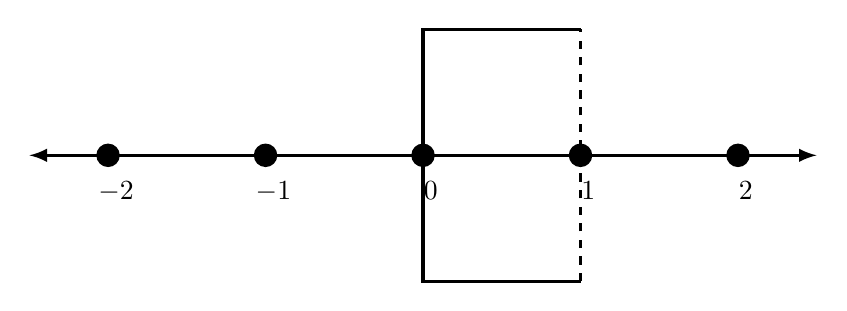
\begin{tikzpicture}[very thick,scale=2]
            \draw[latex-latex] (-2.5,0) -- (2.5,0); 
            \foreach \x in  {-2,-1,0,1,2}
            {
                \node at (\x, 0)[circle,fill,inner sep=3pt]{};
                \draw[shift={(\x+0.05,-0.1)}] node[below] {$\x$};
            }
            \draw[dashed] (1,-0.8) -- (1,0.8);
            \draw (1,0.8) -- (0,0.8) -- (0, -0.8) -- (1, -0.8);
        \end{tikzpicture}}
    \end{center}

    同理,我们可以得到
    \[[1]_R = \{y \in \mathbb{R} \mid (1, y) \in \mathbb{R}\} = \{y \in \mathbb{R} \mid 1 \le y < 2\}\]
    如下图所示:

    \begin{center}
        {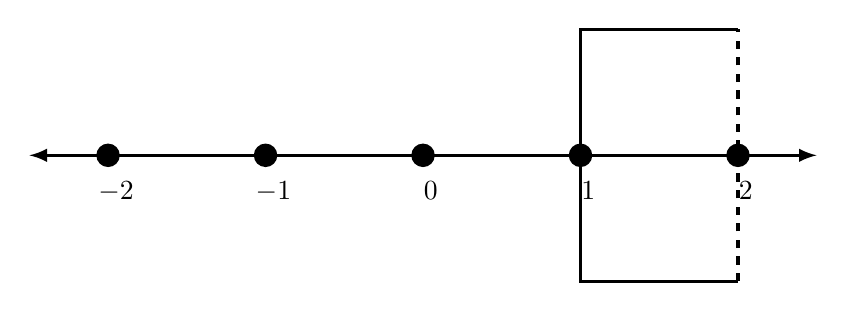
\begin{tikzpicture}[very thick,scale=2]
            \draw[latex-latex] (-2.5,0) -- (2.5,0); 
            \foreach \x in  {-2,-1,0,1,2}
            {
                \node at (\x, 0)[circle,fill,inner sep=3pt]{};
                \draw[shift={(\x+0.05,-0.1)}] node[below] {$\x$};
            }
            \draw[dashed] (2,-0.8) -- (2,0.8);
            \draw (2,0.8) -- (1,0.8) -- (1, -0.8) -- (2, -0.8);
        \end{tikzpicture}}
    \end{center}
\end{example}

请注意,这两个集合是互不相交的,因为第一个集合不包含 $1$,而第二个集合包含 $1$。此外,\emph{每个}实数都\emph{恰好属于一个}这样的区间。例如,我们可以说
\[\pi \in [3]_R, e \in [2]_R, -1.5 \in [-2]_R,\frac{1}{2} \in [0]_R\]
请注意,\emph{等价类}的定义并没有要求我们必须用一个元素来\emph{表示}该类。例如,我们也可以这样说
\[[0]_R = \Big[\frac{1}{2}\Big]_R\]
因为这两个集合是相等的,它们包含相同的元素。任何``向下取整'' 为 $0$ 的实数在 $R$ 下都与 $0$ 相关,因此在 $R$ 下也与 $\frac{1}{2}$ 相关,因为它们的向下取整都是 $0$。

多探索一下这个例子,尝试说服自己,这个划分属性在这里确实有效。在下一部分,我们将在你的帮助下正式证明这一事实的普遍性!由于接下来的讨论会比较抽象,我们建议你多通过实际例子来理解。尝试在另一个集合上定义一个等价关系。它的等价类是什么?你能理解为什么它们会构成一个划分吗?

\subsubsection*{等价类划分集合}

我们已经探讨了等价类\emph{划分}集合的思想,接下来让我们来正式定义这个概念。我们需要先给出一个定义,然后再证明一个定理!这个定理本质上是一个``当且仅当''定理,我们将证明其中一个方向,另一个方向留作练习。

\begin{definition}
    设 $R$ 为集合 $A$ 上的等价关系,关系 $R$ 下等价类的集合记作 $A / R$,即 $A$ \dotuline{模 (modulo)} $R$。也就是说
    \[A / R = \{[x]_R \mid x \in A\}\]
    换种写法是
    \[A / R = \{X \subseteq A \mid \exists x \in A \centerdot X = [x]_R\}\]
\end{definition}

在我们证明重要结果之前,先来看几个例子来理解这些概念。在每个例子中,我们要判断是否存在等价关系,检验等价类,并思考模运算的作用。\\

\begin{example}
    再次考虑定义在实数集 $\mathbb{R}$ 上的关系 $R$ ,其定义为 $(x, y) \in R \iff \lfloor x \rfloor = \lfloor y \rfloor$。我们之前已经讨论过为什么这是一个等价关系,现在让我们来研究一下它的等价类。

    根据定义,任何两个相关的元素都有相同的等价类。例如,$[0]_R = [0.5]_R = [0.999]_R$。同样地,$[3.5]_R = [3.75]_R$ ,以及 $[-\pi]_R = [-4]_R$ ,但 $[\pi]_R = [4]_R$。每个实数 $x \in \mathbb{R}$ 都有一个对应的等价类 $[x]_R$,而模运算的思想是通过只考虑必要的等价类来简化 $R$ 的表示。由于 $[0]_R = [0.5]_R = [0.333]_R$ 等等,我们可以用一个集合 $[0]_R$ 来代表所有这些相同的集合。因此,我们可以表示
    \[\mathbb{R} / R = \{\dots, [-2]_R, [-1]_R, [0]_R, [1]_R, [2]_R, \dots \}\]
    实际上,$\mathbb{R} / R$ 可以看作是整数集 $\mathbb{Z}$。然而,我们通常写作 $\mathbb{R} / R ``='' \mathbb{Z}$ 是因为这种等式并不完全准确。特别是,我们还没有严格推导出实数或整数,仅仅严格定义了自然数 $\mathbb{N}$。在这里,我们只是观察到等价类集合与整数集合之间的某种对应关系。我们可以将一个对应到另一个,反之亦然,但这并不意味着它们在技术上是\emph{相等的}。

    不过没关系!这个例子的主要目的是指出 $\mathbb{R} / R$ 是一个等价类的集合。记住,当我们写下一个集合时,顺序和重复是无关紧要的。也就是说, $\{1, 3, 5, 3, 1\}$ 在集合意义上等于 $\{1, 3, 5\}$。它们具有\emph{相同元素},因此是\emph{相同对象}。在当前的上下文中,我们不需要在集合  $\mathbb{R} / R$ 中同时包含 $[0]_R$ 和 $[0.5]_R$,因为它们是同一个对象;在我们的元素列表中重复该对象没有任何意义。

    通常,我们会关注识别等价类的形式并提供一些定性的描述。特别是,我们会经常思考在 $A/R$ 中有多少个等价类。我们还会关注这些类的大小。它们都是一样大的吗?是不是有些类只有几个元素,而有些类则是无穷大的?为什么会这样?这些类元素的``描述''是否大致相同?

    在这个特定的例子中,我们发现 $\mathbb{R} / R$ 中的所有等价类在形式上非常相似。有无限多个等价类 --- 每个整数 $\mathbb{Z}$ 的元素都是一个 --- 它们都是无穷大的,包含一个实数区间。此外,所有这些类的形式都是对于某个 $z \in \mathbb{Z}, [z]_R = \{y \in \mathbb{R} \mid z \le y < z + 1\}$。从这个意义上说,这些等价类都是\emph{性质相似}的。
\end{example}

\begin{example}
    在所有人的集合 $S$ 上定义关系 $B$ 为 $(x, y) \in B \iff x \;\text{和}\; y \;\text{同一个月出生}$。那么 $(\text{欧拉}, \text{庞加莱}) \in B$ 且 $(\text{Paul Erdös}, \text{Emmy Noether}) \in B$。为什么这是等价关系?任何人都与自己相同月份出生(自反性)。如果两个人同一月份出生,那么他们的出生月份是相同的(对称性)。如果 $x$ 和 $y$ 同一月份出生,$y$ 和 $z$ 同一月份出生,那么 $x$ 和 $z$ 也是同一月份出生(传递性)。

    (注意:通常由``有相同的……''或``是相同的……''定义的关系是等价关系。)

    在这个关系下,等价类对应的是月份。因为我们用出生月份来区分人群,一个等价类就是一组同月出生的人。例如,Paul Erdös 和 Emmy Noether 都是三月出生,所以我们可以说 $\text{Emmy Noether} \in [\text{Paul Erdös}]_B$ 这个等价类。这个等价类\emph{对应于}三月,但请注意,它是根据集合 $S$ (所有人)中的特定元素定义的。

    如果我们定义 $M$ 为所有三月出生的人的集合,那么我们可以说 $M = [\text{Paul Erdös}]_B$。综合这些观察,我们可以得出结论:按出生月份划分人的集合,记为 $S/B$,由 $12$ 个集合组成,每个集合对应一个不同月份,并包含所有在那个月份出生的人。
\end{example}

\begin{example}
    考虑所有有序实数对的集合 $\mathbb{R} \times \mathbb{R}$。我们通过定义两个对何时\emph{相关}来定义 $\mathbb{R} \times \mathbb{R}$ 上的关系 $R$。具体来说,我们定义
    \[\big((x, y),(u, v)\big) \in R \iff x = u\]
    也就是说,当平面上的两点第一个坐标相同时,它们在关系 $R$ 下是相关的。想想为什么这是一个等价关系?从几何上讲,这个关系只关心一个点所在的垂直于 $y$ 轴的直线。理解这一点后,你可以很容易地``看出''并解释为什么 $R$ 是一个等价关系,而严格证明这一点只需要多写一些内容和符号。(试试看!)

    这也使我们能够轻松描述和可视化这个关系下的等价类。所有在同一垂线上的点都属于同一个等价类,我们可以通过查看这些垂线与水平轴的交点来索引这些类。例如,$(1, 3) \in [(1, 0)]_R$,因为点 $(1, 3)$ 和 $(1, 0)$ 位于同一条垂线上。我们可以用这种方式表示\emph{每一个}等价类:$[(x, 0)]_R$,其中 $x \in \mathbb{R}$。
\end{example}

\begin{center}
    {\begin{tikzpicture}[very thick,scale=2]
        \draw[latex-latex] (-1.5,0) -- (2.5,0); 
        \draw[latex-latex] (0,-1.5) -- (0,3.5); 
        \foreach \x in  {1,2}
        {
            \node at (\x, 0)[circle,fill,inner sep=3pt]{};
            \draw[shift={(\x+0.25,-0.1)}] node[below] {$(\x, 0)$};
        }
        \foreach \y in  {1,2,3}
        {
            \node at (0, \y)[circle,fill,inner sep=3pt]{};
            \draw[shift={(-0.15, \y)}] node[left] {$(0, \y)$};
        }
        \draw[dashed] (1,-1.5) -- (1,3.5);
        \node at (1, 3)[circle,fill,inner sep=3pt]{};
        \draw[shift={(1.15, 3)}] node[right] {$(1, 3)$};
        \draw[shift={(1.15, 1.5)}] node[right] {$[(1,0)]_R = \{(1, y)\}$};
    \end{tikzpicture}}
\end{center}

因此,在某种意义上,等价类的集合 $(\mathbb{R} \times \mathbb{R})/R$ 与实数轴 $\mathbb{R}$ 是``等同的''!通过忽略第二个坐标,我们可以将平面上的所有点压缩到水平轴上。从数学上讲,有一种方法可以更精确地表达这个想法,但在此我们无法正式讨论。简单来说,$\mathbb{R} \times \mathbb{R}$ 上的这个关系产生的等价类由 $\mathbb{R}$ 表示,这其中存在一些有趣的现象。

这里有另一个 $\mathbb{R} \times \mathbb{R}$ 上的关系。定义 $S$ 为
\[\big((x, y),(u, v)\big) \in S \iff \sqrt{x^2+y^2} = \sqrt{u^2+v^2}\]
回想一下基本的几何和代数知识,你可能会发现表达式 $\sqrt{x^2 + y^2}$ 描述的是点 $(x, y)$ 到原点 $(0, 0)$ 的距离。(在数学中,我们称这种表达式为\emph{度量 (metric)}。)因此,这个关系表明,当两点到原点的距离相同时,它们是等价的。从视觉上来看,这解释了为什么 $S$ 是一个等价关系,并且展示了等价类是以原点为中心的圆。因此,我们可以通过这些圆的一个显著特征 --- 它们的\emph{半径} $r \ge 0$,来描述集合 $(\mathbb{R} \times \mathbb{R})/S$ 的元素。因此,在 $S$ 下的等价类集合与非负实数集合是``等同的''!

\begin{center}
    {\begin{tikzpicture}[very thick,scale=2]
        \draw[latex-latex] (-3,0) -- (3,0); 
        \draw[latex-latex] (0,-3) -- (0,3); 
        \foreach \x in  {-2,-1,0,1,2}
        {
            \node at (\x, 0)[circle,fill,inner sep=3pt]{};
            \node at (0, \x)[circle,fill,inner sep=3pt]{};
        }
        \draw[dashed] (0,0) circle (1);
        \draw[dashed] (0,0) circle (2);
        \draw[shift={(0.8, -0.7)}] node[right] {$[(1,0)]_S$};
        \draw[shift={(0.8, -0.9)}] node[right] {$r=1$};
        \draw[shift={(1.7, 1.5)}] node[right] {$[(2,0)]_S$};
        \draw[shift={(1.7, 1.3)}] node[right] {$r=2$};
    \end{tikzpicture}}
\end{center}

这听起来有点奇怪,对吧?我们从一个二维集合开始,关联成对的点,并整理出等价类,结果得到了一个一维集合。(注意:我们这里还没有正式的方法来定义\emph{维度},但你应该能理解我们的意思。)回顾一下上面在 $\mathbb{R}^2$ 上定义的关系 $R$。如果我们只在 $\mathbb{R}^2$ 的``右半部分''定义这个关系,也就是所有第一个坐标非负的点,那么等价类的集合也会和非负实数集合``相同''。从哪个角度看,这个集合和 $(\mathbb{R} \times \mathbb{R})/S$ 是``相同''的呢?这个问题合理吗?我们该如何\emph{证明}此说法?这些都是非常有趣的问题,我们鼓励你思考一下这些问题!

不要过于纠结于这些概念和问题。关键在于:等价类的集合构成底层集合的\textbf{划分}。

现在我们已经看过了若干例子,接下来我们来陈述(并证明!)一些关于等价关系的重要结论。主要是,这些定理说明了我们一直暗示的观点,即等价关系会将集合划分成相应的等价类。不过,令人惊讶的是,我们还有一个有趣的结论:给定任意一个划分,我们可以为其定义一个等价关系!

\begin{theorem}\label{theorem6.4.10}
    设 $R$ 为集合 $A$ 上的等价关系。则属于 $A/R$ 的集合构成 $A$ 的划分。也就是说,它们是非空的,互不相交的,它们的并集是 $A$。
\end{theorem}

\begin{proof}
    见习题 \ref{exc:exercises6.7.13}
\end{proof}

我们将在本章末尾的习题 \ref{exc:exercises6.7.13} 中带你完成这个结论的证明。我们之前研究的例子应该可以帮助你直观地理解为什么这个定理是正确的,而通过详细地推导证明过程,你将对其背后的数学严谨性有一个扎实的理解。

\subsubsection*{划分产生等价关系}

现在,我们来看一个类似且重要的结论,这是前一个定理的逆命题。为了更好地理解这个定理,我们先看一个例子,这个例子还将为我们提供定理证明的概要。\\

\begin{example}
    考虑集合 $S=[6]$。定义集合
    \[\mathcal{F} = \{ \{1, 4\}, \{2, 3, 5\} , \{6\} \}\]
    注意,$\mathcal{F}$ 是 $S$ 的一个划分,因为这些集合是互不相交的,非空的,且它们的并集是 $S$。如果有一种等价关系 $R$,使得我们在考虑 $S/R$ 时得到这些集合,那不是很好吗?事实上,确实存在这样的关系!尽管我们可能无法像之前那样,以一种优雅的方式定义它们,例如通常的``$(x, y) \in R \iff x \;\text{和}\; y \;\text{具有某种共同属性}$''。不过,既然我们已经有了划分,就可以用它来定义关系。具体来说,划分集合就是等价类。划分本身建立了等价类的结构,我们只需通过 $(x, y) \in R \iff x \;\text{和}\; y \;\text{属于同一个划分集合}$ 来定义等价关系 $R$。

    在本例中,我们可以定义 $S_1 = \{1, 4\} , S_2 = \{2, 3, 5\} , S_3 = \{6\}$,则我们可以定义 $R$
    \[(x, y) \in R \iff \exists i \in [3] \centerdot (x \in S_i \land y \in S_i)\]
\end{example}

想一想为什么这种方法有效。你能理解为什么这是一个等价关系吗?你知道等价类是什么吗?

现在我们准备陈述并证明这个定理。

\begin{theorem}\label{theorem6.4.12}
    设 $S$ 为集合,并设 $\mathcal{F}$ 为集合 $S$ 的划分。则存在等价关系 $R$ 使得 $S/R=\mathcal{F}$。
\end{theorem}

正如我们之前提到的,这个结果完全依赖于一个事实:划分是一组集合,这些集合正是我们要定义的等价类。我们只需要证明``$x$ 和 $y$ 相关当且仅当 $x$ 和 $y$ 属于同一个划分集合''这个关系是一个等价关系。这并不难!在阅读我们的证明之前,试着自己勾画一下证明的细节吧!

\begin{proof}
    设 $\mathcal{F}$ 为集合 $S$ 的划分。这意味着我们有一个索引集 $I$,且
    \[\mathcal{F} = {S_i \mid i \in I}\]
    其中集合 $S_i$ 满足 $S_i \subseteq S$ 且 $S_i \ne \varnothing$ 且
    \[\bigcup_{i \in I} S_i = S \quad \text{且} \quad \forall i, j \in I \centerdot i \ne j \implies S_i \cap S_j = \varnothing\]
    定义 $S$ 上的关系 $R$ 为
    \[(x, y) \in R \iff \exists i \in I \centerdot (x \in S_i \land y \in S_i)\]
    我们要证明 $R$ 是等价关系。

    \begin{itemize}
        \item 设 $x \in S$ 是任意固定的。由于 $S_i$ 的集合覆盖 $S$,因此我们知道 $\exists i \in I \centerdot x \in S_i$。给定这样的 $i$,则必然有 $x \in S_i$ 且 $x \in S_i$,所以 $(x,x) \in R$。因此 $R$ 具有自反性。
        \item 设 $x, y \in S$ 是任意固定的。假设 $(x, y) \in R$。这意味着 $\exists i \in I \centerdot (x \in S_i \land y \in S_i)$。给定这样的 $i$,则必然有 $y \in S_i \land x \in S_i$,所以 $(y,x) \in R$。因此 $R$ 具有对称性。
        \item 设 $x, y, z \in S$ 是任意固定的。假设 $(x, y) \in R$ 且 $(y, z) \in R$。这意味着 $\exists i \in I \centerdot (x \in S_i \land y \in S_i)$ 且 $\exists j \in I \centerdot (y \in S_j \land z \in S_j)$。给定这样的 $i,j$,注意 $y \in S_i \land y \in S_j$,而对于任意不同的 $i,j, S_i \cap S_j = \varnothing$,因此 $i=j$(否则会出现 $y \in \varnothing$,而这是不可能的!)由于 $x \in S_i, y \in S_i, z \in S_i$,所以 $(x,z) \in R$。因此 $R$ 具有传递性。
    \end{itemize}
    由于上面三个性质成立,所以 $R$ 是一个等价关系!

    $S/R$ 的等价类写做 $[x]_R$,其中 $x \in S$。因为 $\mathcal{F}$ 是 $A$ 的分割,对于某个 $i, x \in S_i$,所以对于某个 $i, [x]_R = S_i$。因此所有等级类等于某集合 $S_i$。

    类似地,任意集合 $S_i \ne \varnothing$,所以 $\exists x \in S_i$,因此存在对应的等价类 $S_i=[x]_R$。因此,每个等价类都是形如 $S_i$ 的集合,反之亦然。
\end{proof}

这表明,任何划分都可以很好地对应一个等价关系及其等价类!


% !TeX root = ../../../book.tex

\subsection{更多示例}

在掌握这两个定理后,让我们通过若干关系示例来加深理解。对于每个例子,判断其是否为等价关系:如果是,则描述其等价类;如果不是,则根据定理说明不是的原因。

\begin{example}
    先从一个简单的例子开始。\\
    回顾示例 \ref{ex:example6.2.9} 定义的相等关系。我们已经解释过,``$=$''在任意集合上都是等价关系,其等价类即各元素自身构成的单元素集。例如,在集合 $\mathbb{N}$ 中,$[1]_{=} = \{1\}, [2]_{=} = \{2\}$,依此类推。所有等价类都是\emph{单元素集}(集合中只有一个元素)。
\end{example}

\begin{example}
    再来看一个相对简单的例子。\\
    回顾示例 \ref{ex:example6.2.5} 中定义的整数集 $\mathbb{Z}$ 上的奇偶关系。这是一个等价关系,让我们来证明这一点。

    \begin{proof}
        设 $a, b, c \in \mathbb{Z}$ 为任意整数。
        \begin{itemize}
            \item \textbf{自反性}:不难发现 $(a,a) \in R$,因为 $a$ 与其自身有相同的奇偶性。因此 $R$ 具有自反性。
            \item \textbf{对称性}:假设 $(a,b) \in R$,则 $a$ 和 $b$ 具有相同的奇偶性。显然,$b$ 和 $a$ 也具有相同的奇偶性,故 $(b,a) \in R$。因此 $R$ 具有对称性。
            \item \textbf{传递性}:假设 $(a,b) \in R$ 且 $(b,c) \in R$。
            \begin{itemize}
                \item 若 $a$ 是奇数,则 $b$ 和 $c$ 也都是奇数。
                \item 若 $a$ 是偶数,则 $b$ 和 $c$ 也都是偶数。
            \end{itemize}
            无论哪种情况,$a$ 和 $c$ 都具有相同的奇偶性,故 $(a,c) \in R$。因此 $R$ 具有传递性。
        \end{itemize}
        综上,由于 $R$ 具有自反性、对称性和传递性,所以 $R$ 是一个等价关系。
    \end{proof}

    这意味着等价类集合 $\mathbb{Z}/R$ 构成 $\mathbb{Z}$ 的划分。让我们来确定该划分。

    考虑 $[0]_R$,它表示所有与 $0$ 奇偶性相同的整数集合,即全体\emph{偶数}。因此,在此情况下,
    \[\mathbb{Z}/R = \{O_{\mathbb{Z}}, E_{\mathbb{Z}}\}\]
    其中 $O_{\mathbb{Z}}$ 为奇数集,$E_{\mathbb{Z}}$ 为偶数集。这两个等价类都是无穷大的。
\end{example}

\begin{example}
    回顾示例 \ref{ex:example6.2.6} 中定义的 $\mathbb{R}$ 上的顺序关系。该关系是等价关系吗?我们可以通过逐一检验其性质来判断。注意到对于任意 $x \in \mathbb{R}$,均有 $(x, x) \notin R$(因为 $x \nless x$)。因此 $R$ 缺乏自反性,故它不是等价关系。(此外,$R$ 虽具有传递性,但缺乏对称性。)

    为何严格顺序关系不能成为等价关系?自反性对等价关系为何重要?考虑\emph{等价类}的概念:等价关系应将整个集合划分为若干子集,使每个元素都能通过所属子集被标识。若关系不具自反性,则某些元素将不属于其自身的``等价类'',这显然不符合要求!

    (进一步思考:自反的顺序关系 $\le$ 是否为等价关系?请说明理由。)
    
    换言之,$\mathbb{R}$ 上的``$<$''关系无法将实数集划分。结合定理 \ref{theorem6.4.10} 的\emph{逆否命题},可推知 ``$<$''\emph{不是}等价关系。
\end{example}

\begin{example}
    定义 $\mathbb{R} \times \mathbb{R}$ 上的关系 $\sim$ 为
    \[(x, y) \sim (u, v) \iff x \le u \land y \le v\]
    即使不逐条检验性质,我们也可以推断出它是否是等价关系。为此,我们选取集合中的一个特定元素,并查看与该特定元素相关的所有元素。在下图中,我们使用 $(1, 1)$ 作为这个特定元素。

    \begin{center}
        {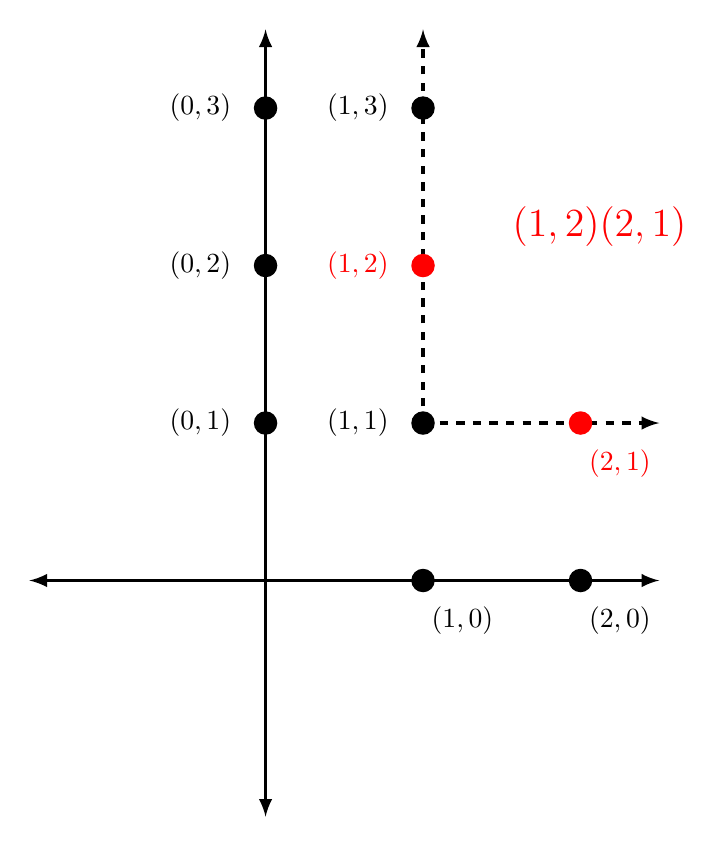
\begin{tikzpicture}[very thick,scale=2]
            \draw[latex-latex] (-1.5,0) -- (2.5,0); 
            \draw[latex-latex] (0,-1.5) -- (0,3.5); 
            \foreach \x in  {1,2}
            {
                \node at (\x, 0)[circle,fill,inner sep=3pt]{};
                \draw[shift={(\x+0.25,-0.1)}] node[below] {$(\x, 0)$};
                
            }
            \foreach \y in  {1,2,3}
            {
                \node at (0, \y)[circle,fill,inner sep=3pt]{};
                \draw[shift={(-0.15, \y)}] node[left] {$(0, \y)$};
            }
    
            \draw[dashed,-latex] (1,1) -- (2.5,1); 
            \draw[dashed,-latex] (1,1) -- (1,3.5); 
            \foreach \y in  {1,3}
            {
                \node at (1, \y)[circle,fill,inner sep=3pt]{};
                \draw[shift={(0.85, \y)}] node[left] {$(1, \y)$};
            }
    
            \node[red] at (1, 2)[circle,fill,inner sep=3pt]{};
            \draw[color=red, shift={(0.85, 2)}] node[left] {$(1, 2)$};
            \node[red] at (2, 1)[circle,fill,inner sep=3pt]{};
            \draw[color=red, shift={(2.25, 0.9)}] node[below] {$(2, 1)$};
    
            \draw[color=red, font=\Large, shift={(1.5, 2.25)}] node[right] {$(1,2) \nsim (2,1)$};
        \end{tikzpicture}}
    \end{center}

    请注意,$\sim$ 要求一个点必须位于另一点的``右上方''方可关联。同时,由于不等式是``$\le$'',因此第二个点不必\emph{严格}位于上方或右侧。

    我们可以从上图看到,$(1, 2) \sim (1, 1)$(因为 $1 \le 1$ 且 $1 \le 2$),同理 $(1, 1) \sim (2, 1)$。故 $(1, 2)$ 与 $(2, 1)$ 均与 $(1, 1)$ 关联。若 $\sim$ 是\emph{等价关系},则 $(2, 1)$ 与 $(1, 2)$ 必须彼此关联(因为同属 $(1, 1)$ 的等价类)。然而遗憾的是,$(1, 2) \nsim (2, 1)$,因为后者位于前者的``左下方'',不满足 $\sim$ 的定义。

    这意味着所有与 $(1, 1)$ 关联的元素\textbf{无法}构成``封闭集合'',从数学上讲,这些元素的集合不是一个等价类。因此,$\sim$ \textbf{不是}一个等价关系。

    请进一步分析 $\sim$ 的性质:是否具有自反性?是否具有对称性?是否具有传递性?请说明理由。此过程将再次验证 $\sim$ 不是一个等价关系。建议遇到新定义的关系时采用类似的分析:若能明确其``等价类'',则有助于理解等价关系的构造;若不能,则可积累反例构造的经验。
\end{example}

\subsubsection*{[选学] $\mathbb{Z}$ 是如何从 $\mathbb{N} \times \mathbb{N}$ 上的等价关系生成的}

回忆第 \ref{ch:chapter03} 章的习题:要求证明自然数对的特定性质,并声称此过程构建了整数集。重审视习题 \ref{exc:exercises3.11.22},其最后三部分要求证集合 $P = \mathbb{N} \times \mathbb{N}$ 上的关系 $R$ 是等价关系(已证其自反性、对称性及传递性)。

还记得第 \ref{ch:chapter03} 章中的那道复杂习题吗?它要求证明自然数对的性质,并声称此过程证明了整数的存在性。重新审视习题 \ref{exc:exercises3.11.22},你会发现问题的最后三部分要求证明集合 $R$ 是集合 $P = \mathbb{N} \times \mathbb{N}$ 上的\textbf{等价关系}。仔细阅读一下!你已经证明了 $R$ 具有自反性、对称性和传递性。

该练习表明(此处略去细节)任何负整数都可以表示为两个整数之差为该负整数的\textbf{等价类}。也就是说
\[-1 \;\text{``$=$''}\; [(1, 2)]_R = \{(1, 2),(2, 3),(3, 4), \dots \}\]
同理
\[-3 \;\text{``$=$''}\; [(1, 4)]_R = \{(1, 4),(2, 5),(3, 6), \dots \}\]
以上只是一个直观的解释,从数学上讲并不严格,但核心思想就在于此!


% !TeX root = ../../../book.tex

\subsection{习题}

\subsubsection*{温故知新}

以口头或书面的形式简要回答以下问题。这些问题全都基于你刚刚阅读的内容,所以如果忘记了具体的定义、概念或示例,可以回去重读相关部分。确保在继续学习之前能够自信地回答这些问题,这将有助于你的理解和记忆!

\begin{enumerate}[label=(\arabic*)]
    \item \emph{等价关系}需要满足哪些性质?
    \item 什么是等价类?等价类中的所有元素必须满足什么条件?
    \item 给定集合 $S$ 和 $S$ 上的等价关系 $R$,等价类的集合必须满足什么条件?
\end{enumerate}

\subsubsection*{小试牛刀}

尝试回答以下问题。这些题目要求你实际动笔写下答案,或(对朋友/同学)口头陈述答案。目的是帮助你练习使用新的概念、定义和符号。题目都比较简单,确保能够解决这些问题将对你大有帮助!

\begin{enumerate}[label=(\arabic*)]
    \item 回顾 \ref{sec:section6.2.5} 节习题 \ref{exc:exercises6.2.2} 中定义的关系。我们在该习题中定义 $\mathbb{Z}$ 上的关系 $\bigstar$ 为
    \[\forall x, y \in \mathbb{Z} \centerdot x \;\bigstar\; y \iff 3 \mid x - y\]
    你之前已经证明了它确实是一个等价关系。现在,请描述一下 $\mathbb{Z}/\bigstar$ 的等价类。有多少个等价类?每个等价类有多大?你能列出它们的元素或描述它们的特征吗?
    \item 回顾 \ref{sec:section6.2.5} 节习题 \ref{exc:exercises6.2.3} 中定义的关系。我们在该习题中定义 $\mathbb{Z}$ 上的关系 $\sim$ 为
    \[\forall x, y \in \mathbb{Z} \centerdot x \sim y \iff 3 \mid x + 2y\]
    你之前已经证明了它确实是一个等价关系。现在,请判别并描述 $\mathbb{Z}/\sim$ 的等价类。有多少个等价类?每个等价类有多大?你能列出它们的元素或描述它们的特征吗?对比上一题,你有什么发现?
    \item 考虑集合 $[5]=\{1,2,3,4,5\}$。定义 $[5]$ 上的关系 $\approx$ 为,对于任意 $x,y \in [5]$
    \[x \approx y \iff \vert x^2 - y^2 \vert \le 5\]
    对于任意 $x \in [5]$,设 $S(x)$ 为满足 $x \approx y$ 且 $y \in [5]$ 的所有元素的集合。
    \begin{enumerate}[label=(\alph*)]
        \item 写出集合 $S(1), S(2), S(3), S(4), S(5)$ 的所有元素。
        \item 通过观察这些集合,你能判断 $\approx$ 是否是一个等价关系吗?你是怎么判断的?
        \item 通过证明或证伪自反性、对称性和传递性,来证明 $\approx$ 是否是一个等价关系。
    \end{enumerate}
    \item 考虑集合 $\mathbb{N} \times \mathbb{N}$。定义该集合上的关系 $\sim$ 为
    \[(a, b) \sim (c, d) \iff a + b = c + d\]
    判断该关系否是一个等价关系。如果是,请可视化地描述其等价类。
\end{enumerate}

\newpage
% !TeX root = ../../../book.tex
\section{模算术}

你可能已经接触过一种自然而常见的等价关系,即整数上的\emph{同余}关系。这是对``奇偶性''等价关系的直接推广,它基于某个特定属性对整数进行分类。在此,我们将通过定义整数的某些性质来扩展这一概念,并引入多个等价类。我们还将探讨一些有趣的结论,这些结论利用同余关系使问题的证明变得更加简便(甚至成为可能!)。

% !TeX root = ../../../book.tex

\subsection{定义与示例}

\subsubsection*{整除性}

我们将从一个我们已经多次见过的定义开始。

\begin{definition}
    设 $a,b \in \mathbb{Z}$。我们说 $a$ 整除 $b$ 是指 $b$ 可以被 $a$ 整除,即 $\exists k$ 使得 $b = ak$,或者等价地,$\frac{b}{a} \in \mathbb{Z}$(排除 $a=b=0$ 的情况)。记作 $a \mid b$。
\end{definition}

注意,这个定义表明每个整数都能整除 $0$(例如,$5 \mid 0$),但 $0$ 除了自己之外不能整除任何数(例如,$0 \nmid 5$ 但 $0 \mid 0$)。想一想这是否符合你对``整除''的直觉理解,同时也满足了给定的定义。另外,这里也考虑了负数的情况,因为存在量词意味着\emph{整数} $k \in \mathbb{Z}$。因此,$-2 \mid 4$ 和 $8 | -24$ 也成立。

现在,像 $2 \nmid 5$ 这样的表达告诉我们一些关于整数 $2$ 和 $5$ 之间关系的信息,但并不能涵盖所有情况。我们知道没有整数 $k$ 可以满足 $2k = 5$,但这并没有说明我们到底能多接近。显然,$k = -100$ 是一个糟糕的估计,但 $2 \times 2 = 4$ 和 $2 \times 3 = 6$ 都非常接近 $5$……对于这样的小数字,这似乎很明显,我们可以手工验证,但对于巨大的数字呢?我们知道 $7 \nmid 100000$(为什么?想想质数……),但我们如何解决这个``找到使 $7k$ 最接近 $100000$ 的 $k$''这个问题呢?我们怎么知道是否有一个具体的答案?会不会有两个同样``合理''的答案,就像 $2 \nmid 5$ 一样?

关于上面第二个问题,为了简化,我们希望限制答案,使其只有一个合理的选项。这是为了避免在找到一个答案后还要担心是否有其他答案。因此,我们将采用\emph{价格猜猜猜}\footnote{价格猜猜猜 (The Price Is Right) 是美国历史上风行时间最长的一档电视节目。--- 译者注}的规则:我们寻找\emph{最接近但不超过}目标值的答案。比如在 $2 \nmid 5$ 的例子中,我们认为 $k = 2$ 是最佳估计,因为 $4 < 5$。同理,在 $7 \nmid 100000$ 的例子中,我们认为 $k = 14285$ 是最佳估计,因为 $7 \times 14285 = 99995 < 100000$。(注意,在这种情况下,有一个``更接近''的估计,但它超过了目标值,因此我们不考虑它。)

这就引出了我们如何得到这样的估计。给定 $a, b \in \mathbb{Z}$,我们可以查看 $a$ 的越来越大的倍数,直到超过 $b$;在此之前的那个最大倍数就是最佳估计。估计的``准确性''范围在 $0$ 到 $a - 1$ 之间,当 $a$ 能整除 $b$ 时,准确性为 $0$。(注意:``超过''是指顺序关系 $>$,所以要仔细考虑这在负数中的应用。比如,$2 \nmid -3$ 而 $2 \times -2 = -4$ 被认为是最佳估计,因为 $-4 \le -3$。)以下引理总结了关于逐步查看 $a$ 的倍数直到找到 $b$ 的最佳估计的思路,并声明在我们设定的约束条件下,总会有唯一解。

\begin{lemma}[除法算法]\label{lemma6.5.2}
    设 $a,b \in \mathbb{Z}$。则 $\exists k, r \in \mathbb{Z}$ 使得 $ak + r = b$,其中 $0 \le r \le a - 1$。换句话说,对于任意两个整数,总能找到一个 $a$ 的倍数,使得它与 $a$ 的乘积最接近 $b$ 而不超过 $b$,同时还存在一个唯一的余数。我们把这个 $r$ 称为``$b$ 除以 $a$ 的余数'' 或 ``$b$ 被 $a$ 除的余数''。
\end{lemma}

我们会频繁使用余数的概念。具体来说,我们将比较两个除法的余数,并基于余数定义一种关系。稍后我们会详细介绍这些内容。首先,请你证明这个重要的引理!

\begin{proof}
    留作习题 \ref{exc:exercises6.7.14}。
\end{proof}

之所以称之为除法\emph{算法},是因为它暗示了一种\emph{找到}这些倍数和余数的\emph{过程}。这种方法虽然简单但非常有效,就是\emph{反复应用减法}。也就是说,给定 $a$ 和 $b$,我们可以不断地从 $b$ 中减去 $a$,例如先得到 $b - a$,再得到 $b - 2a$,然后是 $b - 3a$……依此类推,直到剩下一个介于 $0$ 和 $a$ 之间的余数。\\

\begin{example}
    让我们通过一个例子来展示这个过程。假设 $a = 8, b = 62$。我们不断地从 $62$ 中减去 $8$,结果是:
    \[62, 54, 46, 38, 30, 22, 14, 6\]
    我们停在 $6$ 上,因为它满足 $0 \le 6 < a = 8$,这表明 $r = 6$。我们还注意到,我们总共从 $b$ 中减去了 $7$ 次 $a$,因为列表中有八个项,其中第一项是 $b - 0 \cdot a$。因此,我们可以写出:
    \[\underbrace{62}_{b} = \underbrace{7}_{k} \cdot \underbrace{8}_{a} + \underbrace{6}_{r}\]
\end{example}

这里的重点是有一种方法可以找到这个余数,并且这个余数是唯一的。有了这个结果,我们可以用它来定义某些 $\mathbb{Z}$ 上的关系。接下来,我们将展示这些关系都是等价关系,并具体看看它们的\emph{等价类}是多么有用!

\subsubsection*{模 $n$ 同余}

\begin{definition}\label{def:definition6.5.4}
    设 $n \in \mathbb{N}$。我们定义 $\mathbb{Z}$ 上的关系 $R_n$ 为 $(a,b) \in R_n$ 当且仅当 $a$ 和 $b$ 除以 $n$ 时有相同的余数,即
    \[(a,b) \in R_n \iff n \mid a-b\] 
    写法上,我们也将其写成
    \[a \equiv b \mod n\]
    读作``$a$ 与 $b$ \dotuline{模 $n$ 同余}''。(口头上,我们通常将 ``modulo'' 简化为 ``mod''。)
\end{definition}

\begin{remark}
    我们在定义中提到,``$a$ 和 $b$ 除以 $n$ 后有相同的余数''等同于$n \mid a - b$''。为什么会这样呢?这并非定义本身的原因,而是需要一些证明的。稍后你将在习题 \ref{exc:exercises6.7.15} 中进行这个证明。
\end{remark}

\begin{remark}
    在实际应用中(例如解决问题和证明其他结论时),我们会这样使用这个定义:已知 $a ≡\equiv b \mod n$ 意味着我们可以将 $a$ 表示为 $n$ 的倍数加上 $b$。
\end{remark}

我们来看一下为什么这是成立的。假设它们的余数都为 $r$,这意味着存在 $k, \ell \in \mathbb{Z}$ 使得
\[a = kn + r \quad\text{且}\quad b = \ell n + r\]
(它们有相同的余数,但 $n$ 的倍数可能不同。)通过相减来解出 $r$ 这样我们就能得到等式
\[a - kn = b - \ell n\]
然后移项并提取公因式可得
\[a = (k - \ell)n + b\]
瞧!$(k - \ell)n$ 是 $n$ 的倍数,而第二项只有 $b$ 本身。这说明 $a$ 是 $n$ 的倍数加上 $b$。

通常情况下,$b$ 可能并不是 $a$ 除以 $n$ 后的余数;特别是当 $b$ 不满足余数要求 $0 \le r \le a - 1$ 时,就会出现这种情况。

让我们总结一下这个观点,并写下我们将来会用到的定义形式。这是我们在证明或举例中引用\emph{模 $n$ 同余}定义时会用到的陈述:

\setlength{\fboxrule}{2pt}
\begin{center}
\fcolorbox{olivegreen}{white}{%
    \parbox{0.8\textwidth}{%
        \[a \equiv b \mod n \iff \exists m \in \mathbb{Z} \centerdot a=mn+b\]
    }
}
\end{center}

\begin{example}
    让我们通过考察几个较小的 $n$ 值,来看看这些关系的具体表现。

    \begin{itemize}
        \item 设 $n=1$。关系 $R_1$ 会是什么样?这个问题实际上有些无聊,因为任何整数除以 $1$ 的余数都是 $0$,所以每个整数都可以和其他任意整数相关联。也就是说,$\forall x,y \in \mathbb{Z} \centerdot (x, y) \in R_1$。因为这个关系相对不那么有趣,因此数学家们几乎不会讨论``模 $1$''这个话题。
        \item 设 $n=2$。关系 $R_2$ 就是我们之前定义的``奇偶关系''。想想为什么会这样。当我们把任意整数 $a$ 除以 $2$ 时,余数只能是 $0$ 或 $1$。如果 $a$ 和 $b$ 除以 $2$ 的余数都是 $0$,那么它们都是偶数;如果余数都是 $1$,那么它们都是奇数。(回想一下我们在第 \ref{ch:chapter03} 章中的定义,\emph{奇数}和\emph{偶数}是通过\emph{存在}声明来定义的:例如,当且仅当 $\exists k \in \mathbb{Z}$ 使得 $x = 2k$ 时,$x$ 为偶数。这正是除法算法的结果:当且仅当 $x$ 除以 $2$ 的余数为 $0$ 时,$x$ 为偶数,因为我们可以找到一个整数 $k$,使得 $x = 2k$。)\\
        现在,想想同余的另一种表述。如果两个整数都是偶数,那么它们的差也是偶数!也就是说,$a \equiv b \mod 2 \iff a - b \mid 2$;即 $a$ 和 $b$ 都是偶数(或者都是奇数)当且仅当它们的差也是偶数。(注意:我们还没有\emph{证明}这种表述确实等价于余数的定义。我们将在这个例子之后立即进行证明。)
        \item 设 $n=3$。例如,$0 \equiv 9 \mod 3, -1 \equiv 2 \mod 3$ 以及 $4 \equiv 28 \mod 3$。一般来说,只要在行尾加上``$\mod 3$''(或其他数),我们可以连接多个同余语句。当这样做时,整行都按照模 $3$ 处理。例如,以下语句在符号上是有效的,在数学上也是成立的:
        \[-100 \equiv -1 \equiv 8 \equiv 311 \equiv -289 \equiv 41 \mod 3\]
        (虽然我们不确定为什么需要写这样的陈述,但这样做是完全可以的!)
        \item 设 $n=10$。自然数除以 $10$ 的余数就是它的最后一位数字,也就是个位数字!这样我们就可以轻松地比较两个数的模 $10$ 余数。例如,$12 \equiv 32 \equiv 448237402 \mod 10$;而 $37457 \not\equiv 38201 \mod 10$。\\
        但对于\emph{负数}的情况就有所不同了。因为我们定义余数时,是取\emph{不超过}目标值的最大倍数。例如,$-1 \equiv 9 \mod 10$,这是因为 $-1= (-1) \cdot 10 + 9$,而 $9 = (0) \cdot 10 + 9$。它们的余数都是 $9$,需要加到某个 $10$ 的倍数上。请思考以下陈述的具体细节:
        \[-3 \equiv 17 \equiv -33 \equiv 107 \mod 10\]
    \end{itemize}
\end{example}

\subsubsection*{符号}

需要强调的是:在数学中,\textbf{mod} 是一种关系,而不是运算符或函数。在计算机科学和编程中,你可能会看到类似``$5$ mod $3 = 2$''的表达,这表示``$5$ 除以 $3$ 的余数是 $2$''。(在许多编程语言中,这可能表示为 \verb|5 % 3 = 2|。)在这里,我们不会这样写。我们使用 $\mod$ 和 $\equiv$ 符号表示某种\textbf{等价},因为我们讨论的数字不一定\emph{相等}。如果我们表达的等价链在某个自然数 $n$ 下是有意义的,我们会在行末写上``$\mod n$''来指出这一点。在这个意义上,$\mod$ 更像是一个\emph{修饰符},用来表示``这一行的所有陈述仅在除以 $n$ 的余数上有意义''。因此,我们可以写类似这样的表达
\[100 \equiv 97 \equiv 16 \equiv 4 \equiv z \cdot w \equiv 1 \equiv x - y \equiv -2 \equiv -8 \mod 3\]
这表示当考虑 $\mod 3$ 时,所有这些数字和表达式都是等价的。我们并没有断言它们是相等的,也没有断言它们在其他情况下是等价的。行末的 ``$\mod 3$'' 表示``我们只在整数模 $3$ 的范围内讨论。''

(问题:你能找到 $x, y, z, w \in \mathbb{Z}$ 使上面的等式成立吗?)

\subsubsection*{三个重要引理}

在这里,我们将要求你证明两个重要结论:首先,证明模 $n$ 同余可以用\emph{可除性}来等价理解;其次,证明这些关系是等价关系。在阅读本节时,请完成这些对应的练习。如果你已经掌握了这些细节,下一节关于这些关系下的等价类的内容会更容易理解。在这两个证明之后,我们还会展示并证明另一个结果。在讨论等价类之前,最后一个例子是一个有趣的算术问题,用同余可以轻松解决,但如果手工计算就不那么容易了。

\begin{lemma}\label{lemma6.5.8}
    在定义 \ref{def:definition6.5.4} 中,模 $n$ 同余的两种表述确实是等价的。也就是说,对于所有 $a, b \in \mathbb{Z}$ 和所有 $n \in \mathbb{N}$,
    \[a, b \;\text{除以}\; n \;\text{余数相同} \iff n \mid a - b\]
\end{lemma}

\begin{proof}
    见习题 \ref{exc:exercises6.7.15}
\end{proof}

\begin{lemma}\label{lemma6.5.9}
    对于任意 $n \in \mathbb{N}, R_n$ 是 $\mathbb{Z}$ 上的等价关系。
\end{lemma}

\begin{proof}
    见习题 \ref{exc:exercises6.7.16}
\end{proof}

感谢你证明了这些引理!$\smiley{}$ 现在我们知道模 $n$ 同余是一个等价关系(因此我们可以讨论等价类)。我们还了解到,要判断两个整数 (如 $a$ 和 $b$) 是否模 $n$ 同余,只需确定 $a - b$ 是否是 $n$ 的\emph{倍数}即可。这是一种验证同余关系是否成立的有效方法。

下一个引理告诉我们,在``模 n''的情况下进行加法和乘法\textbf{运算},结果仍然正确。如果我们有两个关于整数的等式,并将它们相加,结果仍然是正确的。也就是说,如果 $a + b = c$ 且 $d + e = f$,我们可以得到 $a + b + d + e = c + f$。这个引理说明,同样的原理适用于模 $n$ 的同余关系。同理,我们可以对同余关系进行乘法运算,并且同余关系仍然成立。

虽然这个引理的证明并不复杂,但我们会为你证明它,因为最近我们让你做了太多工作了。

\begin{lemma}[模算术引理 (Modular Arithmetic Lemma, 简称 MAL)]\label{lemma6.5.10}
    设 $n \in \mathbb{N}$。设 $a,b,r,s \in \mathbb{Z}$ 为任意固定整数。假设 $a \equiv r \mod n$ 且 $b \equiv s \mod n$。则
    \begin{align*}
        a + b &\equiv r + s \mod n \\
        a \cdot b &\equiv r \cdot s \mod n
    \end{align*}
\end{lemma}

(这个引理告诉我们,我们只需要处理余数。无论给定的 $a$ 和 $b$ 是什么,我们可以将它们化简为余数 $r$ 和 $s$,然后对这些余数进行计算。因为 $0 \le r, s \le n - 1$,所以它们相对于 $a$ 和 $b$ 来说是较小的,这使得我们在实际操作中可以更快地进行算术运算。以下证明保证了这种方法在所有情况下都有效。)

\begin{proof}
    假设 $a \equiv r \mod n$ 且 $b \equiv s \mod n$。这意味着 $\exists k, \ell \in \mathbb{Z}$ 使得
    \begin{align*}
        a &= kn + r \\
        b &= \ell n + s \\
    \end{align*}
    将上面两个等式相加得
    \[a + b = (kn + r) + (\ell n + s) = (k + \ell)n + (r + s)\]
    因为我们可以将 $a+b$ 表示为 $n$ 的倍数加上余数 $r+s$,所以 $a + b \equiv r + s \mod n$。\\ \\
    将上面两个等式相乘得
    \[a \cdot b =  (kn + r) \cdot (\ell n + s) = k\ell n^2 + (ks + \ell r)n + r \cdot s = n \cdot (k\ell n + ks + \ell r)+r \cdot s\]
    因为我们可以将 $a \cdot b$ 表示为 $n$ 的倍数加上余数 $r \cdot s$,所以 $a \cdot b \equiv r \cdot s \mod n$。
\end{proof}

\begin{remark}
    请注意,我们在此没有提到\textbf{减法}和\textbf{除法},而是只讨论了加法和乘法。这有两方面的原因。首先,减法实际上是``加一个负数''。因此,这个引理表明我们可以通过以下两个步骤来\emph{减去}两个同余:
    \begin{enumerate}[label=(\arabic*)]
        \item 将其中一个同余乘以 $-1$(应用\emph{乘法}引理)
        \item 将结果相加(应用\emph{加法}引理)
    \end{enumerate}
    看到它是如何\emph{同时}利用这两个引理的结果了吗?很巧妙,对吧?

    第二个原因稍微复杂一些。实际上,在模 $n$ 的情况下没有``除法''这种运算。主要原因是我们这里讨论的范围仅限于\emph{整数},而除法可能会产生非整数的\emph{有理数}。例如,我们知道 $4 \equiv 7 \mod 3$,但这是否意味着 $\frac{4}{2} \equiv \frac{7}{2} \mod 3$ 呢?这又意味着什么呢?一个整数(例如 $2$)怎么可能与一个非整数(例如 $\frac{7}{2}$)同余呢?正是因为这个原因,我们在 $\mathbb{Z}$ 模 $n$ 的环境中不讨论\textbf{除法}运算。

    关于这个``除法''问题,其实还有一些更细微的细节。我们会在 \ref{sec:section6.5.3} 节讨论\emph{乘法逆元}时详细说明。现在为了避免引起混淆,我们暂时不讨论这些细节。简单来说,我们将会发展出一种在某些特定情况下类似于模 $n$ 除法的方法。

    同时,为了确保我们只讨论\emph{整数},我们将\emph{仅}涉及加法和乘法。
\end{remark}

\subsubsection*{两个实用例子}

我们还不确定是否已经让你相信模算术的用处。为了确保我们已经证明了同余作为等价关系的概念既有数学趣味又有实用价值,我们将在这里举两个有趣且实用的例子。第一个例子是一个简单的问题,用模算术可以比用``标准''算术更容易解决。第二个例子是一个你可能以前用过但从未考虑过其原理的巧妙技巧。我们会证明它的有效性!\\ \\

\begin{example}
    考虑如下问题:
    \begin{center}
        \parbox{0.8\textwidth}{%
            \textbf{问题:}

            是否\emph{存在}自然数 $k$,使得 $5^k$ 恰好比 $7$ 的倍数多 $1$?

            如果存在,这样的自然数最小是多少?

            你能描述所有满足该条件的自然数吗?
        }
    \end{center}
    我们可以尝试通过代入 $k$ 的值来回答这些问题,看看会发生什么。然而,你很快会注意到,计算大指数会很麻烦,而要确定一个大数是否正好比$7$ 的某个倍数多 $1$ 会更加困难!如果你愿意的话可以继续尝试一下。甚至可以使用计算器。看看你能否解决这个问题!

    不过,我们更倾向于这样做:多次利用模算术引理 (Modular Arithmetic Lemma, MAL)。指数运算只是重复的乘法,因此我们可以反复应用该引理的乘法结论。其核心思想是,我们可以不断乘以 $5$,并在此过程中将所有结果模 $7$。也就是说,我们只需要找到一个比 $7$ 的倍数多 $1$ 的数 --- 即模 $7$ 同余 $1$ 的数 --- 而不需要立即知道该数具体是多少,只需判断它是否满足这一性质。接下来我们将展示此过程。

    我们从 $5^1 \equiv 5 \mod 7$ 开始。将其乘以 $5$ 得
    \[5^2 \equiv 5 \cdot 5 \equiv 25 \equiv 4 \mod 7\]
    我们发现 $25 = 21 + 4$,并且知道 $21$ 是 $7$ 的倍数,从而得出上述结论。(当数字较小时,我们常常可以通过简单观察进行算术运算。也就是说,我们可以直接心算。当然,如果不确定,我们也可以使用除法算法,从 $25$ 中不断减去 $7$,直到剩下余数。)

    接着我们发现
    \[5^3 \equiv 5^2 \cdot 5 \equiv 4 \cdot 5 \equiv 20 \equiv 6 \mod 7\]
    我们发现,通过``观察''可以知道 $20 = 14+6$。请注意,我们现在知道 $5^3$ 模 $7$ 的余数是多少,但并不需要实际计算 $5^3 = 125$ 然后再化简。因为我们在此过程中已经将所有数字都化简到模 $7$ 的余数,所以省去了大量计算。具体来说,我们总是将数字化简到\emph{小于} $7$ 的范围内,因此在任何情况下我们需要处理的最大数也只会在 $20$ 到 $30$ 之间。这真是太方便了!让我们继续看看接下来会得到什么结果:
    \begin{align*}
        5^4 &\equiv 5^3 \cdot 5 \equiv 6 \cdot 5 \equiv 30 \equiv 2 \mod 7 \\ 
        5^5 &\equiv 5^4 \cdot 5 \equiv 2 \cdot 5 \equiv 10 \equiv 3 \mod 7 \\
        5^6 &\equiv 5^5 \cdot 5 \equiv 3 \cdot 5 \equiv 15 \equiv 1 \mod 7 
    \end{align*}
    这正是我们要找的结果!我们已经确定 $5^6$ 比 $7$ 的某个倍数多 $1$。这种方法比直接计算 $5^6 = 15625$ 并找出 $15625 = 7 \cdot 2232 + 1$ 要简单得多,不是吗?

    这已经解决了前两个问题:我们发现存在 $5$ 的幂满足所需性质,并且由于我们是从 $k = 1$ 开始逐步找到它的,因此可以确定这是最小的结果。第三个问题留给你来研究,即描述所有满足该性质的数。你可以继续我们的过程,乘以 $5$ 并进行化简。你是否注意到了某种模式?它是什么?尝试提出一个猜想并加以证明!(我们稍后会回到这个例子……)
\end{example}

\begin{example}\label{ex:example6.5.13}
    考虑数字 $474$。它是 $3$ 的倍数吗?也许你只是将它的各位数字加起来 --- $4 + 7 + 4$ 等于 $15$ --- 并注意到 $15$ 是 $3$ 的倍数,从而得出结论 $474$ 也必然是 $3$ 的倍数。(当然,你也可以通过长除法计算出 $474 = 3 \cdot 158$。)为什么你可以这样做呢?是不是因为你的老师在三年级时告诉了你这个方法,你就记住了?这对我们来说远远不够!$\smiley{}$

    这里,我们将严格\textbf{证明},一个自然数 $x$ 能被 $3$ 整除当且仅当其各位数字之和也能被 $3$ 整除。(在证明过程中,包含了一些用具体例子来详细说明的语句。这些例子是为了帮助你理解我们所写的内容,我们将其放在括号中,以提醒你,仅仅展示一个例子并不是一个正式的证明。例子可以帮助读者更容易理解实际的证明,但仅凭一个例子不足以证明这个普遍适用的结论。)

    \begin{proof}
        设 $x \in \mathbb{N}$ 为任意固定自然数。我们可以用它的十进制展开形式来表示这个数字
        \[x= \sum_{k=0}^{n-1} x_k \cdot 10^k\]
        其中 $n$ 为数字 $x$ 的位数,$x_k$ 为对应 $10^k$ 位的数字,所以 $0 \le x_k \le 9$。(也就是说,$x_k$ 是从右往左读取的 $x$ 的第 $(k + 1)$ 位数。)

        (例如,我们可以将 $47205$ 写做 $47205=4 \cdot 10^4+7 \cdot 10^3+2 \cdot 10^2+0 \cdot 10^1+5 \cdot 10^0$。本例中,$x_0 = 5, x_1=0, x_3=2$。)

        整除技巧声称
        \[x \equiv 0 \mod 3 \iff \sum_{k=1}^{n-1} x_k \equiv 0 \mod 3\]

        为了证明这一点,我们将考虑十进制展开模 $3$。注意,由于 $10=9+1$,因此 $10 \equiv 1 \mod 3$。因此
        \[\forall k \in \mathbb{N} \cup \{0\} \centerdot 10^k \equiv 1^k \equiv 1 \mod 3\]

        (这源于模算术引理和 $1^k = 1$ 对任意 $k$ 都成立的事实。思考一下!)

        这使我们能够在十进制展开中用 $1$ 替换 $10$ 的幂!因此

        \begin{align*}
            x \equiv 0 \mod 3 &\iff \sum_{k=0}^{n-1} x_k \cdot 10^k \equiv 0 \mod 3 &\text{将}\; x \;\text{重写为十进制展开形式}\\
            &\iff \sum_{k=0}^{n-1} x_k \cdot 1^k \equiv 0 \mod 3 &\text{因为}\; 10 \equiv 1 \mod 3 \\
            &\iff \sum_{k=0}^{n-1} x_k \equiv 0 \mod 3
        \end{align*}

        以上完成了该声明的证明。
    \end{proof}

    (注意,$3 \mid 47205$ 是因为 $3 \mid (4 + 7 + 2 + 0 + 5)$,也就是说 $3 \mid 18$。实际上,$15735 \cdot 3 = 47205$)。

    有趣的是,我们实际上在这里证明了一个\textbf{更强的}结论。因为前面的陈述\emph{当且仅当}陈述,所以我们知道更多的信息:如果 $x$ 的各位数字之和不是 $3$ 的倍数,那么 $x$ 也不是 $3$ 的倍数,并且有\emph{相同的余数}。例如,$3 \nmid 122$,因为 $3 \nmid 5$;此外,$5 \equiv 2 \mod 3$,所以我们知道 $122 \equiv 2 \mod 3$。(确实,$122 = 3 \cdot 40 + 2$。)

    我们还可以找到并证明类似的关于 $9$ 和 $11$ 的整除技巧(虽然 $11$ 的技巧稍微复杂一些)。甚至还有一个关于 $7$ 的技巧,但很难用文字表达。这些概念将在本章的习题中进一步探讨。
    
    记住这个结论及其证明。这是一个可以在聚会上炫耀的小技巧。你可以挑战你的朋友:他们真的知道\textbf{为什么}这个技巧有效吗?你却知其然也知其所以然!
\end{example}


% !TeX root = ../../../book.tex

\subsection{模 $n$ 等价类}

你已经证明了(参见引理 \ref{lemma6.5.9})模 $n$ 同余确实是集合 $\mathbb{Z}$ 上的等价关系。你还证明了(参见定理 \ref{theorem6.4.10})等价关系的等价类能够\emph{划分}底层集合。结合这两个结果,我们知道模 $n$ 同余可以将 $\mathbb{Z}$ 划分成若干个等价类。那么,我们如何表示这些等价类呢?每个类的代表元素应该如何选择呢?

让我们先从两个更简单的问题开始:
\begin{enumerate}[label=(\arabic*)]
    \item $\mathbb{Z}$ 模 $n$ 有多少个等价类?
    \item 这些等价类有多``大''?
\end{enumerate}

\subsubsection*{有多少等价类?}

要回答问题 (1),我们只需要回忆一下如何定义除以 $n$ 的余数。根据除法算法(参见引理 \ref{lemma6.5.2}),当我们将一个数除以 $n$ 时,余数 $r$ 必须满足 $0 \le r \le n-1$。这意味着余数最多有 $n$ 种可能:$0,1,2 \dots$ 一直到 $n-1$。(即,$r \in [n-1] \cup \{0\}$。)那么,是否确实存在余数为这些数的数呢?当然存在,因为我们可以直接使用这些数本身。例如,当我们将 $n-1$ 除以 $n$ 时,余数就是 $n-1$(因为 $n-1 < n$)。由此可见,$\mathbb{Z}$ 模 $n$ 的等价类恰好有 $n$ 个。

通过相同的观察,我们可以确定这些等价类的\emph{代表元素}。由于 $a \equiv b \mod n$ 表示 $a$ 和 $b$ 除以 $n$ 具有相同的余数,那么我们可以声明这两个数属于由这个\emph{余数}所代表的等价类。这个余数 $r$ 必须满足 $0 \le r \le n-1$,我们写做 $a, b \in [r]_{\mod n}$ 来表示 $a$ 和 $b$ 属于由余数 $r$ 代表的等价类(下标 ``$\mod n$'' 表示余数是 $n$ 除得的结果)。

\subsubsection*{这些类有多大?}

让我们通过一个具体的例子来思考这个问题,例如 $n = 4$。对于一个整数 $z \in \mathbb{Z}$ 属于余数为 $0$ 的等价类,这意味着什么?也就是说,如果我们知道 $z \in [0]_{\mod 4}$,我们可以得出哪些关于 $z$ 的结论?

根据模运算的定义,我们知道这意味着 $z$ 被 $4$ 除后余数为 $0$。也就是说,$z$ 是 $4$ 的\emph{倍数}。在整数集 $\mathbb{Z}$ 中,$4$ 的倍数有多少个呢?答案是无穷多个!例如,$4, 8, 12, 16, \dots ,$ 以及 $0,-4,-8,-12,\dots$。因此,集合 $[0]_{\mod 4}$ 是一个\emph{无限}集合。

那么,$z \in [1]_{\mod 4}$ 又意味着什么呢?余数为 $1$ 意味着 $z$ 可以表示为 $4k + 1$;也就是说,\emph{存在}一个整数 $k$,使得 $z$ 可以这样表示。那 $k$ 可以取什么值呢?实际上,任意 $k \in \mathbb{Z}$ 都会生成一个这样的 $z$,因此我们可以考虑 $k = 0, k = 1, k = 2, \dots$ 以及 $k = -1, k = -2, \dots$ 看看结果如何。我们发现这会生成一个集合
\begin{align*}
    [1]_{\mod 4} &= \{\dots , -7, -3, 1, 5, 9, \dots \} \\
    &= \{z \in \mathbb{Z} \mid \exists k \in \mathbb{Z} \centerdot z = 4k + 1\} \\
    &= \{4k + 1 \mid k \in \mathbb{Z}\}
\end{align*}
请注意,我们一开始用了 ``$\dots$'' 符号来展示我们发现的模式,随后又用集合构建符(以两种不同的方式)重写了这个集合。

这也是一个无限集合。你可以尝试使用其他余数(无论是除以 $4$ 还是其他任意整数 $n$),来发现这些集合都是\emph{无限的}。(此外,我们尚未\emph{正式}定义什么是无限集合,但我们依赖的是共同的直觉。如果你想更好地理解,可以这样想:这个集合是无限的,因为我们可以列出它的所有元素,并找到一个生成所有元素的模式,但这个过程在有限时间内无法结束。)

\subsubsection*{$\mathbb{Z}$ 模 $n$ 的划分}

我们可以根据对等价类的观察,来总结 $\mathbb{Z}$ 模 $n$ 的等价类的标准表示。已知有 $n$ 个等价类,每个等价类包含无穷多个元素。每个等价类对应于整数除以 $n$ 的余数。由于余数必须满足 $0 \le r \le n-1$,我们将集合 $\{0, 1, 2, \dots , n-1\} = [n-1] \cup \{0\}$ 作为标准代表集合。

余数为 $r$ 的等价类包含所有除以 $n$ 余 $r$ 的整数。换句话说,所有 $z \in [r]_{\mod n}$ 的元素都是 $n$ 的某个倍数加上 $r$。也就是说,我们可以通过从 $r$ 开始不断加上或减去 $n$ 来生成等价类的所有元素。这样,同一等价类中的任何两个元素相差 $n$ 的倍数。

\setlength{\fboxrule}{2pt}
\setlength\fboxsep{5mm}
\begin{center}
\noindent \fcolorbox{blue}{white}{%
    \parbox{0.85\textwidth}{%
        \linespread{1.5}\selectfont
        \textcolor{blue}{\textbf{$\mathbb{Z}$ 模 $n$ 等价类:}}\\
        给定 $n \in \mathbb{N}$,恰好存在 $n$ 个等价类
        \[[0]_{\mod n}, [1]_{\mod n}, [2]_{\mod n}, \dots ,[n-1]_{\mod n}\]
        它们的特点是:
        \begin{align*}
            [0]_{\mod n} &=  \{\dots, -2n, -n, 0, n, 2n, \dots \} \\
            &= \{z \in \mathbb{Z} \mid \exists k \in \mathbb{Z} \centerdot z = kn\}\\
            [1]_{\mod n} &=  \{\dots, -2n+1, -n+1, 1, n+1, 2n+1, \dots \} \\
            &= \{z \in \mathbb{Z} \mid \exists k \in \mathbb{Z} \centerdot z = kn+1\}\\
            [2]_{\mod n} &=  \{\dots, -2n+2, -n+2, 2, n+2, 2n+2, \dots \} \\
            &= \{z \in \mathbb{Z} \mid \exists k \in \mathbb{Z} \centerdot z = kn+2\}\\
            &\vdots \\
            [n-1]_{\mod n} &=  \{\dots, -n-1, -1, n-1, 2n-1, 3n-1, \dots \} \\
            &= \{z \in \mathbb{Z} \mid \exists k \in \mathbb{Z} \centerdot z = kn+(n-1)\}\\
            &= \{z \in \mathbb{Z} \mid \exists \ell \in \mathbb{Z} \centerdot z = \ell n-1\}
        \end{align*}
    }
}
\end{center}

以上是我们所有观察结果的全面总结。下面是一些具体 $n$ 值的例子。

\begin{itemize}
    \item 考虑 $n=2$。等价类为
        \begin{align*}
            [0]_{\mod 2} &= \{z \in \mathbb{Z} \mid \exists k \in \mathbb{Z} \centerdot z = 2k\} =  \{\text{偶数}\}\\
            &= \{\dots, -6, -4, -2, 0, 2, 4, 6 \dots \}\\
            [1]_{\mod 2} &= \{z \in \mathbb{Z} \mid \exists k \in \mathbb{Z} \centerdot z = 2k+1\} =  \{\text{奇数}\}\\
            &= \{\dots, -5, -3, -1, 1, 3, 5, 7 \dots \}
        \end{align*}
    \item 考虑 $n=3$。等价类为
        \begin{align*}
            [0]_{\mod 3} &= \{z \in \mathbb{Z} \mid \exists k \in \mathbb{Z} \centerdot z = 3k\} =  \{3 \;\text{ 的倍数}\}\\
            &= \{\dots, -9, -6, -3, 0, 3, 6, 9 \dots \}\\
            [1]_{\mod 3} &= \{z \in \mathbb{Z} \mid \exists k \in \mathbb{Z} \centerdot z = 3k+1\} =  \{3 \;\text{ 的倍数加 }\; 1\}\\
            &= \{\dots, -8, -5, -2, 1, 4, 7, 10 \dots \}\\
            [2]_{\mod 3} &= \{z \in \mathbb{Z} \mid \exists k \in \mathbb{Z} \centerdot z = 3k+2\} =  \{3 \;\text{ 的倍数加 }\; 2\}\\
            &= \{\dots, -7, -4, -1, 2, 5, 8, 11 \dots \}
        \end{align*}
    \item 考虑 $n=4$。等价类为
        \begin{align*}
            [0]_{\mod 4} &= \{z \in \mathbb{Z} \mid \exists k \in \mathbb{Z} \centerdot z = 4k\} =  \{4 \;\text{ 的倍数}\}\\
            &= \{\dots, -12, -8, -4, 0, 4, 8, 12 \dots \}\\
            [1]_{\mod 4} &= \{z \in \mathbb{Z} \mid \exists k \in \mathbb{Z} \centerdot z = 4k+1\} =  \{4 \;\text{ 的倍数加 }\; 1\}\\
            &= \{\dots, -11, -7, -3, 1, 5, 9, 13 \dots \}\\
            [2]_{\mod 4} &= \{z \in \mathbb{Z} \mid \exists k \in \mathbb{Z} \centerdot z = 4k+2\} =  \{4 \;\text{ 的倍数加 }\; 2\}\\
            &= \{\dots, -10, -6, -2, 2, 6, 10, 14 \dots \}\\
            [3]_{\mod 4} &= \{z \in \mathbb{Z} \mid \exists k \in \mathbb{Z} \centerdot z = 4k+3\} =  \{4 \;\text{ 的倍数加 }\; 3\}\\
            &= \{\dots, -9, -5, -1, 3, 7, 11, 15 \dots \}
        \end{align*}
\end{itemize}

\subsubsection*{使用等价类}

为什么这很有用?为什么我们要带你了解整数模特定等价关系集合的构建?

$\mathbb{Z}$ 被这些等价类\textbf{划分}这一点非常重要。因此,每当我们在 $\mathbb{Z}$ 模 $n$ 的背景下进行算术运算时,只需要考虑这些等价类,即余数。我们可以将所有整数简化为 ${0, 1, 2, \dots , n-1}$ 这些数字,因为它们代表了所有整数。这样,我们不需要进行大量大数算术运算再找余数;只需处理这些余数即可。让我们通过几个例子来看看这种划分的实际用处。\\

\begin{example}
    考虑下面的声明:
    \[\forall n \in \mathbb{N} \centerdot 6 \mid n^3 + 5n\]
    我们之前让你通过对 $n$ 进行归纳来证明这个问题!(参见 \ref{sec:section5.7} 节的练习 \ref{exc:exercises5.7.15}) 现在,我们将利用等价类来证明这一点!

    考虑 $\mathbb{Z}$ 模 $6$。因为 $\mathbb{N} \subseteq \mathbb{Z}$,根据除以 $6$ 的余数,我们知道每个 $n \in \mathbb{N}$ 必然落在等价类 $[0]_{\mod 6}, [1]_{\mod 6}, [2]_{\mod 6}, [3]_{\mod 6}, [4]_{\mod 6}, [5]_{\mod 6}$ 中的\textbf{一个}。

    我们可以分别检查每种情况。假设 $n$ 属于某个特定的等价类,这样我们就可以计算出 $n^3+5n$ 属于哪个等价类。在每种情况下,我们通过乘法(以及幂运算,即重复乘法)和加法,应用模算术引理 \ref{lemma6.5.10}。
    \begin{align*}
        n \equiv 0 \mod 6 &\implies n^3 + 5n \equiv 0^3 + 5 \cdot 0 \equiv 0 \mod 6 \\
        n \equiv 1 \mod 6 &\implies n^3 + 5n \equiv 1^3 + 5 \cdot 1 \equiv 6 \equiv 0 \mod 6 \\
        n \equiv 2 \mod 6 &\implies n^3 + 5n \equiv 2^3 + 5 \cdot 2 \equiv 18 \equiv 0 \mod 6 \\
        n \equiv 3 \mod 6 &\implies n^3 + 5n \equiv 3^3 + 5 \cdot 3 \equiv 42 \equiv 0 \mod 6 \\
        n \equiv 4 \mod 6 &\implies n^3 + 5n \equiv 4^3 + 5 \cdot 4 \equiv 84 \equiv 0 \mod 6 \\
        n \equiv 5 \mod 6 &\implies n^3 + 5n \equiv 5^3 + 5 \cdot 5 \equiv 150 \equiv 0 \mod 6 
    \end{align*}
    以上每种情况,我们都得到 $n^3 + 5n$ 是 $6$ 的倍数(因为它除以 $6$ 的余数是 $0$)。这说明无论 $n$ 取什么值,$n^3 + 5n$ 都是 $6$ 的倍数。这证明了对于所有 $n \in \mathbb{N}$,该命题成立,从而无需使用归纳论证!
\end{example}

\begin{example}[二次残差]\label{ex:example6.5.15}

    在这个例子中,我们将研究完全平方数。具体来说,我们将探讨完全平方数在被不同的数字除时会产生哪些余数。这个例子非常有趣,因为你会发现,根据除数的不同,余数会呈现出一些独特的模式,你可能会因此想要进一步探索这些模式(如果是这样,那就太好了!)。此外,这个例子还很有用,因为我们的研究会引导我们得出一些其他结果,这些结果在本文和练习中都有证明。特别是,研究完全平方数在探索\textbf{毕达哥拉斯三元组}时非常有帮助;毕达哥拉斯三元组是指满足 $a^2 + b^2 = c^2$ 的整数三元组 $(a, b, c) \in \mathbb{N}^3$。了解完全平方数的性质可以帮助我们证明这些三元组的一些有趣的事实!

    对于以下情况,我们将固定一个特定的 $n \in \mathbb{N}$,然后研究对于每个 $x \in \mathbb{Z}, x^2$ 模 $n$ 的结果。在了解 $\mathbb{Z}$ 模 $n$ 的划分后,我们可以简化为查看所有 $n$ 个可能的模 $n$ 余数,然后平方取模。这些可能的余数称为\textbf{二次残差}(称之为\emph{二次}是因为我们使用完全平方数,称之为\emph{残差}是因为我们寻找余数)。在每种情况下,我们将总结这些可能的二次残差列表。

    $\mathbf{n=2}$:

    我们知道,只有当底数为偶数时,完全平方数才是偶数;只有当底数为奇数时,完全平方数才是奇数。在第 \ref{ch:chapter04} 章中,我们曾通过讨论双向条件陈述、量词和证明技巧来验证这些说法。现在无需重新正式证明这些结论;我们可以通过模运算轻松验证这些结果。\\
    设 $x \in \mathbb{Z}$ 为任意固定整数。
    \begin{itemize}
        \item 首先,假设 $x \equiv 0 \mod 2$ (即 $x$ 为偶数)。则应用模算术引理可得 $x^2 \equiv 0 \mod 2$ (即 $x^2$ 为偶数)。
        \item 其次,假设 $x \equiv 1 \mod 2$ (即 $x$ 为奇数)。则应用模算术引理可得 $x^2 \equiv 1 \mod 2$ (即 $x^2$ 为奇数)。
    \end{itemize}
    因此,$\mathbb{Z}$ 模 $2$ 的划分告诉我们,这是唯一需要考虑的情况。
    \begin{quotation}
        \begin{center}
            \large 模 $2$ 二次残差:$\{0, 1\}$
        \end{center}
    \end{quotation}

    $\mathbf{n=3}$: 

    设 $x \in \mathbb{Z}$ 为任意固定整数。应用模算术引理可得:
    \begin{itemize}
        \item $x \equiv 0 \mod 3 \implies x^2 \equiv 0^2 \equiv 0 \mod 3$
        \item $x \equiv 1 \mod 3 \implies x^2 \equiv 1^2 \equiv 1 \mod 3$
        \item $x \equiv 2 \mod 3 \implies x^2 \equiv 2^2 \equiv 4 \equiv 1 \mod 3$
    \end{itemize}
    \begin{quotation}
        \begin{center}
            \large 模 $3$ 二次残差:$\{0, 1\}$
        \end{center}
    \end{quotation}

    $\mathbf{n=4}$: 

    设 $x \in \mathbb{Z}$ 为任意固定整数。应用模算术引理可得:
    \begin{itemize}
        \item $x \equiv 0 \mod 4 \implies x^2 \equiv 0^2 \equiv 0 \mod 4$
        \item $x \equiv 1 \mod 4 \implies x^2 \equiv 1^2 \equiv 1 \mod 4$
        \item $x \equiv 2 \mod 4 \implies x^2 \equiv 2^2 \equiv 4 \equiv 0 \mod 4$
        \item $x \equiv 3 \mod 4 \implies x^2 \equiv 3^2 \equiv 9 \equiv 1 \mod 4$
    \end{itemize}
    \begin{quotation}
        \begin{center}
            \large 模 $4$ 二次残差:$\{0, 1\}$
        \end{center}
    \end{quotation}

    $\mathbf{n=5}$: 

    设 $x \in \mathbb{Z}$ 为任意固定整数。应用模算术引理可得:
    \begin{itemize}
        \item $x \equiv 0 \mod 5 \implies x^2 \equiv 0^2 \equiv 0 \mod 5$
        \item $x \equiv 1 \mod 5 \implies x^2 \equiv 1^2 \equiv 1 \mod 5$
        \item $x \equiv 2 \mod 5 \implies x^2 \equiv 2^2 \equiv 4 \mod 5$
        \item $x \equiv 3 \mod 5 \implies x^2 \equiv 3^2 \equiv 9 \equiv 4 \mod 5$
        \item $x \equiv 4 \mod 5 \implies x^2 \equiv 4^2 \equiv 16 \equiv 1 \mod 5$
    \end{itemize}
    \begin{quotation}
        \begin{center}
            \large 模 $5$ 二次残差:$\{0, 1, 4\}$
        \end{center}
    \end{quotation}

    $\mathbf{n=6}$: 

    设 $x \in \mathbb{Z}$ 为任意固定整数。应用模算术引理可得:
    \begin{itemize}
        \item $x \equiv 0 \mod 6 \implies x^2 \equiv 0^2 \equiv 0 \mod 6$
        \item $x \equiv 1 \mod 6 \implies x^2 \equiv 1^2 \equiv 1 \mod 6$
        \item $x \equiv 2 \mod 6 \implies x^2 \equiv 2^2 \equiv 4 \mod 6$
        \item $x \equiv 3 \mod 6 \implies x^2 \equiv 3^2 \equiv 9 \equiv 3 \mod 6$
        \item $x \equiv 4 \mod 6 \implies x^2 \equiv 4^2 \equiv 16 \equiv 4 \mod 6$
        \item $x \equiv 5 \mod 6 \implies x^2 \equiv 5^2 \equiv 25 \equiv 1 \mod 6$
    \end{itemize}
    \begin{quotation}
        \begin{center}
            \large 模 $6$ 二次残差:$\{0, 1, 3, 4\}$
        \end{center}
    \end{quotation}

    $\mathbf{n=7}$: 

    设 $x \in \mathbb{Z}$ 为任意固定整数。应用模算术引理可得:
    \begin{itemize}
        \item $x \equiv 0 \mod 7 \implies x^2 \equiv 0^2 \equiv 0 \mod 7$
        \item $x \equiv 1 \mod 7 \implies x^2 \equiv 1^2 \equiv 1 \mod 7$
        \item $x \equiv 2 \mod 7 \implies x^2 \equiv 2^2 \equiv 4 \mod 7$
        \item $x \equiv 3 \mod 7 \implies x^2 \equiv 3^2 \equiv 9 \equiv 2 \mod 7$
        \item $x \equiv 4 \mod 7 \implies x^2 \equiv 4^2 \equiv 16 \equiv 2 \mod 7$
        \item $x \equiv 5 \mod 7 \implies x^2 \equiv 5^2 \equiv 25 \equiv 4 \mod 7$
        \item $x \equiv 6 \mod 7 \implies x^2 \equiv 6^2 \equiv 36 \equiv 1 \mod 7$
    \end{itemize}
    \begin{quotation}
        \begin{center}
            \large 模 $7$ 二次残差:$\{0, 1, 2, 4\}$
        \end{center}
    \end{quotation}

    $\mathbf{n=8}$: 

    设 $x \in \mathbb{Z}$ 为任意固定整数。应用模算术引理可得:
    \begin{itemize}
        \item $x \equiv 0 \mod 8 \implies x^2 \equiv 0^2 \equiv 0 \mod 8$
        \item $x \equiv 1 \mod 8 \implies x^2 \equiv 1^2 \equiv 1 \mod 8$
        \item $x \equiv 2 \mod 8 \implies x^2 \equiv 2^2 \equiv 4 \mod 8$
        \item $x \equiv 3 \mod 8 \implies x^2 \equiv 3^2 \equiv 9 \equiv 1 \mod 8$
        \item $x \equiv 4 \mod 8 \implies x^2 \equiv 4^2 \equiv 16 \equiv 0 \mod 8$
        \item $x \equiv 5 \mod 8 \implies x^2 \equiv 5^2 \equiv 25 \equiv 1 \mod 8$
        \item $x \equiv 6 \mod 8 \implies x^2 \equiv 6^2 \equiv 36 \equiv 4 \mod 8$
        \item $x \equiv 7 \mod 8 \implies x^2 \equiv 7^2 \equiv 49 \equiv 1 \mod 8$
    \end{itemize}
    \begin{quotation}
        \begin{center}
            \large 模 $8$ 二次残差:$\{0, 1, 4\}$
        \end{center}
    \end{quotation}

    我们鼓励你继续研究其他二次残差。你甚至可以尝试编写一个计算机程序来生成这些列表。你发现什么规律了吗?对于给定的 $n \in \mathbb{N}$,模 $n$ 的二次残差有多少个?它们分别是什么?你能否确定某些数字在任何给定的列表中一定会出现或一定不会出现?请尝试探索一下吧!
\end{example}

\begin{example}
    让我们将前一个例子中的思想进行推广,看看在特定情况下\emph{三次残差}的情况如何。
    \begin{quote}
        假设 $x, y, z \in \mathbb{Z}$ 满足 $x^3+y^3=z^3$。\\
        证明值 $\{x, y, z\}$中至少有一个是 $7$ 的倍数。
    \end{quote}
    重申一下我们的目标,我们要证明
    \[x \equiv 0 \mod 7 \lor y \equiv 0 \mod 7 \lor z \equiv 0 \mod 7\]
    为此,让我们来看看模 $7$ 的三次残差有哪些。\\
    设 $x \in \mathbb{Z}$ 为任意固定整数。应用模算术引理可得:
    \begin{itemize}
        \item $x \equiv 0 \mod 7 \implies x^3 \equiv 0^3 \equiv 0 \mod 7$
        \item $x \equiv 1 \mod 7 \implies x^3 \equiv 1^3 \equiv 1 \mod 7$
        \item $x \equiv 2 \mod 7 \implies x^3 \equiv 2^3 \equiv 8 \equiv 1 \mod 7$
        \item $x \equiv 3 \mod 7 \implies x^3 \equiv 3^3 \equiv 9 \cdot 3 \equiv 2 \cdot 3 \equiv 6 \mod 7$
        \item $x \equiv 4 \mod 7 \implies x^3 \equiv 4^3 \equiv 16 \cdot 4 \equiv 2 \cdot 4 \equiv 8 \equiv 1 \mod 7$
        \item $x \equiv 5 \mod 7 \implies x^3 \equiv 5^3 \equiv 25 \cdot 5 \equiv 4 \cdot 5 \equiv 20 \equiv 6 \mod 7$
        \item $x \equiv 6 \mod 7 \implies x^3 \equiv 6^3 \equiv (-1)^3 \equiv -1 \equiv 6 \mod 7$
    \end{itemize}
    (注意,为了简化计算,我们将 $6$ 写成 $-1$ 再模 $7$。)

    我们发现唯一的可能值是 $\{0, 1, 6\}$。

    现在,假设我们有一个方程的解,即我们有 $x, y, z \in \mathbb{Z}$ 使得 $x^3 + y^3 = z^3$。每一项 --- $x^3,y^3,z^3$ 模 $7$ 同余于 $0$ 或 $1$ 或 $6$。让我们来看些例子。
    \begin{itemize}
        \item 假设 $x^3 \equiv 0 \mod 7$。则 $y^3$ 可以与 $0$ 或 $1$ 或 $6$ 模 $7$ 同余,我们只需要让 $x^3$ 落在相同的等价类即可。不管怎样,在这种情况下,我们有 $x^3 \equiv 0 \mod 7$。
        \item 假设 $y^3 \equiv 0 \mod 7$。将上面的论证应用于 $x^3$ 和 $z^3$。不管怎样,在这种情况下,我们有 $y^3 \equiv 0 \mod 7$。
        \item 假设 $x^3 \equiv 1 \mod 7$。\\
            为了引出矛盾而假设 $y^3 \equiv 1 \mod 7$。则 $x^3+y^3 \equiv 1+1 \equiv 2 \mod 7$,但 $2$ 不在模 $7$ 的立方残差中,因此这是不可能的。\\
            然而我们发现 $y^3 \equiv 0 \mod 7$ 是可能的,因为 $x^3+y^3 \equiv 1+0 \equiv 1 \mod 7$。\\
            同时我们发现 $y^3 \equiv 6 \mod 7$ 是可能的,因为 $x^3+y^3 \equiv 1+6 \equiv 7 \equiv 0 \mod 7$。\\
            不管怎样,在这种情况下,我们\emph{至少}有一个立方数 --- 要么是 $y^3$ 要么是 $z^3$ --- 与 $0$ 模 $7$ 同余。
        \item 假设 $y^3 \equiv 1 \mod 7$。将上面的论证应用于 $x^3$ 和 $z^3$。我们发现,不管怎样,至少有一个立方数 与 $0$ 模 $7$ 同余。
        \item 假设 $x^3 \equiv 6 \mod 7$。\\
            为了引出矛盾而假设 $y^3 \equiv 6 \mod 7$。则 $x^3+y^3 \equiv 6+6 \equiv 12 \equiv 5 \mod 7$,但 $5$ 不在模 $7$ 的立方残差中,因此这是不可能的。\\
            然而我们发现 $y^3 \equiv 0 \mod 7$ 是可能的,因为 $x^3+y^3 \equiv 6+0 \equiv 6 \mod 7$。\\
            同时我们发现 $y^3 \equiv 1 \mod 7$ 是可能的,因为 $x^3+y^3 \equiv 6+1 \equiv 7 \equiv 0 \mod 7$。\\
            不管怎样,在这种情况下,我们\emph{至少}有一个立方数 --- 要么是 $y^3$ 要么是 $z^3$ --- 与 $0$ 模 $7$ 同余。
        \item 假设 $y^3 \equiv 6 \mod 7$。将上面的论证应用于 $x^3$ 和 $z^3$。我们发现,不管怎样,至少有一个立方数 与 $0$ 模 $7$ 同余。
    \end{itemize}

    我们现在已经知道,无论是哪种情况,总有\textbf{至少}一个立方数与 $0$ 模 $7$ 同余。具体哪个立方数具有这种性质取决于具体情况(有时可能有多个立方数符合),但总有至少一个。

    这对我们很有帮助,因为我们可以回顾一下立方残差列表,会发现一个有趣的现象:\emph{唯一}一个立方数与 $0$ 模 $7$ 同余的底数本身也与 $0$ 模 $7$ 同余!换句话说,
    \[\forall z \in \mathbb{Z} \centerdot z^3 \equiv 0 \mod 7 \implies z \equiv 0 \mod 7\]
    这意味着,在上述每种情况下,我们至少有一个立方数与 $0$ 模 $7$ 同余,这进一步说明我们至少有一个底数与 $0$ 模 $7$ 同余。通过列出所有可能性并分析一些情况,我们已经证明了这个方程\emph{所有可能解}的一个性质,而无需找到具体的解!
\end{example}

现在,尽管所有工作都已经完成,但我们有个不幸的消息:原方程\emph{唯一}的解是\emph{平凡}解,即 $x = y = z = 0$。就是这样!你可以尝试寻找其他解,但都是徒劳的。这个结果是\textbf{费马大定理}的一个特例,该定理指出,对于方程 $x^k + y^k = z^k$(其中 $k \in \mathbb{N}$),只有当 $k = 1$ 或 $k = 2$ 时,才存在非平凡的整数解(即 $x, y, z \in \mathbb{Z}$);也就是说,当 $k \in \mathbb{N} - \{1, 2\}$ 时,唯一的解是 $x = y = z = 0$。

费马在世时曾提到过这个事实,但他从未发表过证明。他在一个笔记本空白处声称自己有一个简短的证明,但空间不足以写下它,不过我们现在知道这可能并不是真的。费马生活在 1600 年代,但这个定理直到 1990 年代才被证明\footnote{安德鲁·怀尔斯 (Andrew Wiles) 于 1994 年证明了费马大定理。--- 译者注}!而且,这个证明涉及了大量在费马之后逐步发展起来的强大数学工具。

如果我们了解这个定理,就能很轻松地证明这个例子中的陈述了!既然唯一的解是 $x = y = z = 0$,那么显然这些值都是 $7$ 的倍数。然而,这样做既没有趣味,也不能让我们练习模算术和等价类。\\

\begin{example}
    这是另一个涉及立方残差的问题:
    \begin{quote}
        假设 $x, y, z \in \mathbb{Z}$ 满足 $x^3+y^3+z^3=3$。\\
        证明值 $x^3 \equiv y^3 \equiv z^3 \mod 9$。
    \end{quote}

    我们这里讨论的是一个特定的\emph{丢番图方程}。丢番图方程是指那些带有多个变量和整数系数的多项式方程。要解这样的丢番图方程,需要找到一组整数,使得这些整数代入方程后能够成立。在这个问题中,我们要证明方程的任意解都必须使得所有项 --- $x^3, y^3, z^3$ --- 在模 $9$ 同余。

    首先,试着找出该方程的几个解,看看具体的例子。我们提供几个简单的例子帮助你入门:例如 $(x, y, z)$ 可以等于 $(1, 1, 1)$ 或 $(4, 4, -5)$。你发现这些解符合我们要求的性质了吗?你还能找到其他解吗?(这个问题比较难,不用太过在上面投入精力。)

    有趣的是,我们甚至不需要识别所有解的具体形式或找到它们,就可以证明这一结论。我们只需要找出模 $9$ 的立方残差:\\
    设 $x \in \mathbb{Z}$ 为任意固定整数。应用模算术引理可得:
    \begin{itemize}
        \item $x \equiv 0 \mod 9 \implies x^3 \equiv 0^3 \equiv 0 \mod 9$
        \item $x \equiv 1 \mod 9 \implies x^3 \equiv 1^3 \equiv 1 \mod 9$
        \item $x \equiv 2 \mod 9 \implies x^3 \equiv 2^3 \equiv 8 \mod 9$
        \item $x \equiv 3 \mod 9 \implies x^3 \equiv 3^3 \equiv 9 \cdot 3 0 \mod 9$
        \item $x \equiv 4 \mod 9 \implies x^3 \equiv 4^3 \equiv 16 \cdot 4 \equiv (-2) \cdot 4 \equiv -8 \equiv 1 \mod 9$
        \item $x \equiv 5 \mod 9 \implies x^3 \equiv 5^3 \equiv 25 \cdot 5 \equiv (-2) \cdot 5 \equiv -10 \equiv 8 \mod 9$
        \item $x \equiv 6 \mod 9 \implies x^3 \equiv 6^3 \equiv 36 \cdot 6 \equiv 0 \cdot 6 \equiv 0 \mod 9$
        \item $x \equiv 7 \mod 9 \implies x^3 \equiv 7^3 \equiv 49 \cdot 7 \equiv 4 \cdot (-2) \equiv -8 \equiv 1 \mod 9$
        \item $x \equiv 8 \mod 9 \implies x^3 \equiv 8^3 \equiv (-1)^3 \equiv -1 \equiv 8 \mod 9$
    \end{itemize}
    注意,在某些情况下,我们会使用负数来简化计算。这是完全可以的,并且对你大有帮助!例如,与其计算 $4^3 = 64$ 然后模 $9$,我们可以用 $-2$ 来代替 $16$ 以保持数字较小。我们可以随时从任何数中加减 $9$ 的倍数,因此在计算过程中可以这样做,而不是先得到一个大数然后再模 $9$。(当然,$64$ 并不是一个很大的数字,所以这一点似乎不太显著;然而,当你处理更大的数字时,这就非常有用。此外,尽可能将数字简化到个位数,可以减少心算错误的发生!)注意,我们在最右边只看到了三种可能性;模 $9$ 的立方残差为 $\{0, 1, 8\}$。就是这样!

    当然,要使 $x^3 + y^3 + z^3 = 3$ 成立,我们需要 $x^3 + y^3 + z^3 \equiv 3 \mod 9$,因为 $3 \equiv 3 \mod 9$。查看可能的立方残差 --- $0, 1, 8$ --- 我们发现\emph{只有} $1 + 1 + 1$ 等于 $3$。试试其他组合:$0 + 1 + 8 \equiv 9 \equiv 0 \mod 9$ 和 $8 + 8 + 8 \equiv 24 \equiv 6 \mod 9$ 等等。这意味着我们需要 $x^3 \equiv y^3 \equiv z^3 \equiv 1 \mod 9$,才能使 $(x, y, z)$ 成为解。

    在解决这个问题时,我们证明了一个略强的结论。我们不仅知道 $x^3,y^3,z^3$ 必须模 $9$ 同余,它们还必须模 $9$ 同余于 $1$。这比我们原本需要的信息更多了一些。

    现在,事实证明,这个问题还有一个\emph{更强的}结论。实际上,$x \equiv y \equiv z \mod 9$。也就是说,不仅它们的\emph{立方}模 $9$ 同余,它们的\emph{底数}也是模 $9$ 同余的。(注意,这并不意味着底数模 $9$ 同余于 $1$;例如,我们的另一个例子 $(4, 4, -5)$ 就表明情况并非如此。)不幸的是,证明这一点需要涉及很多高等数学,超出了本书的范围。不过,这应该能让你理解,这些``简单''的问题(易描述,小数值,纯整数)实际上需要非常复杂和深奥的数学才能解决。不过,不要把这看作是打击,而是启发:只需一点数学知识,我们就能触及这个问题的表面,这暗示了更为深刻和复杂的基础。

    (如果你感兴趣,这里有一篇论文给出了完整的结论,证明了 $x \equiv y \equiv z \mod 9$ 是必然的:
    \begin{quote}
        \href{http://www.ams.org/journals/mcom/1985-44-169/S0025-5718-1985-0771049-4/S0025-5718-1985-0771049-4.pdf}{http://www.ams.org/journals/mcom/1985-44-169/\\S0025-5718-1985-0771049-4/S0025-5718-1985-0771049-4.pdf}
    \end{quote}
    即便是前两段,你也需要查阅一些定义才能阅读下来。完整阅读下来也需要你学习一些相关的数学知识,可能需要几个月也可能需要几年,具体时间取决于你的兴趣。记住这一点,并在你往后的数学生涯中再回头看看!)
\end{example}


% !TeX root = ../../../book.tex

\subsection{乘法逆元}\label{sec:section6.5.3}

我们之前在证明模算数引理(引理 \ref{lemma6.5.10})时提到过,不会在 $\mathbb{Z}$ 模 $n$ 的背景下讨论``除法''。本节中,我们将重新探讨这个想法,并解释为什么(以及如何)在某些特定情况下``除法''是合理的。然而,我们要强调的是,我们实际上在讨论一个更广泛的\textbf{乘法逆元}的概念,而\textbf{不是}真正的``除法''。我们将首先通过几个启发性例子来解释这一点,然后我们将陈述并证明这些特定情况下的具体结果。

\subsubsection*{整体概念}

给定一个特定的数学对象,它的\textbf{乘法逆元}是另一个对象,当我们将这两个对象``相乘''时,结果为 ``$1$''。这里我们加上引号是因为``相乘''和 ``$1$'' 的含义在不同的语境中可能会有很大差异。\\

\begin{example}
    让我们先考虑一个熟悉的例子。假设我们讨论的是实数集 $\mathbb{R}$,且使用通常的乘法运算。现在我们取数字 $2$。它的乘法逆元是什么?也就是说,是否存在另一个实数 $x$ 使得 $2 \cdot x = 1$?如果存在,它是多少?很明显,$x = \frac{1}{2}$ 是符合要求的!可以注意到 $2 \cdot \frac{1}{2} = 1$。出于这个原因,我们可以写出
    \[2^{-1} = \frac{1}{2} \quad \text{在 }\; \mathbb{R} \;\text{范围内}\]
    当我们把方程两边同时除以 $2$ 时,实际上是在把方程的两边都\emph{乘以} $2$ 的\emph{乘法逆元}。
\end{example}

\begin{example}
    现在让我们考虑一个可能不太熟悉的例子。想象一个挂钟,钟面上有均匀分布的 $12$ 个小时刻度标记。我们将考虑旋转挂钟,所以我们声明标准位置,即顶部 $12$ 点的位置为 ``$1$''。也就是说,这是没有进行额外旋转的标准表示法,所以我们称其为\emph{单位元}。实际上,我们的 ``$1$'' 就是指 ``$0 \degree$ 旋转'' 后的挂钟。

    现在,让我们假设将两个旋转``相乘''只是依次进行旋转。例如,我们先将时钟顺时针旋转 $45 \degree$,然后再顺时针旋转 $90 \degree$。在这个例子中,我们实际上是将 ``$45 \degree$ 旋转'' 和 ``$90 \degree$ 旋转'' \emph{乘}在一起,结果得到 ``$135 \degree$ 旋转''。

    建立这些约定的目的是为了明确我们的上下文、对象、``相乘''的含义以及``1''的定义,从而能够识别任意旋转的\emph{乘法逆元}。如果你仔细想一下,就会发现如果我们将 ``$\theta$ 度旋转'' 与 ``$360-\theta$ 度旋转'' 相乘,那么我们实际上是将时钟旋转了 $360 \degree$,并回到了标准位置,这正是我们在这个上下文中的 ``$1$''。这意味着,在我们当前上下文中
    \[(\theta \;\text{度旋转})^-1 = 360-\theta \;\text{度旋转}\]
\end{example}

这两个例子旨在说明,\emph{逆元}的概念是一个普遍的概念,并不局限于数字\emph{除法}这种标准上下文。事实上,当我们讨论\emph{函数的逆}时,也会看到类似的例子。(在这个上下文中,``相乘''指的是函数的复合,``$1$'' 是指恒等函数。虽然具体内容会在下一章详细介绍,但我们现在提到这一点,是为了让已经熟悉这些概念的读者有一个预先的理解。)

\subsubsection*{互质}

你可能已经熟悉以下定义。我们将在后续的结果中用到它,这个结果将说明在 $\mathbb{Z}$ 模 $n$ 的情况下何时存在乘法逆元,因此我们现在想重申这个定义并展示一些例子。

\begin{definition}
    给定 $x,y \in \mathbb{Z}$,我们说 $x$ 和 $y$ \dotuline{互质}当且仅当它们没有除 $1$ 以外的公因子。
\end{definition}

(\textbf{注意}:``互质'' 表示 $x$ 和 $y$ 彼此互质,并不是说 $x$ ``类似质数''或其他意思。)\\

\begin{example}
    例如,$12$ 和 $35$ 互质,因为 $12 = 2^2 \cdot 3$,而 $35 = 5 \cdot 7$,因此它们没有任何公因数。

    通常,写出\emph{质因数分解}是有帮助的,因为我们实际上是想知道两个数是否有共同的质因数(这意味着它们有公因数)。

    举个反例,$12$ 和 $33$ 不互质,因为 $3 \mid 12$ 且 $3 \mid 33$。
\end{example}

\begin{example}
    这个例子陈述的结果在后面会很有用。

    \textbf{声明}:如果 $p$ 是质数且 $a$ 不是 $p$ 的倍数,那么 $p$ 和 $a$ 互质。

    (也就是说,如果 $p$ 是质数且 $p \nmid a$,则 $p$ 和 $a$ 互质。)

    让我们来看看为什么这是正确的!

    \begin{proof}
        设 $p$ 为质数且 $a \in \mathbb{Z}$。假设 $p \nmid a$。

        由于 $p \nmid a$,所以 $a$ 的质因数中不包含 $p$。因为 $p$ 是质数,因此 $a$ 的质因数也不会整除 $p$。这意味着 $a$ 和 $p$ 没有共同的质因数,因此它们互质。
    \end{proof}

    这非常方便!特别是,我们现在知道,只要 $p$ 是质数,那么\textbf{所有}数字 $1, 2, 3, \dots , p-1$ 都与 $p$ 互质。
\end{example}

\subsubsection*{定义与示例}

我们来讨论一下在 $\mathbb{Z}$ 模 $n$ 的情况下,什么是\emph{乘法逆元}。这里的``乘法''指的是常规乘法,但所有结果都要模 $n$。另外,``$1$'' 实际上是对应于 $1$ 的\emph{等价类}。在这种情况下,我们说对于任意 $x \in \mathbb{Z}$,当且仅当 $xy \equiv 1 \mod n$ 时,$x$ 的乘法逆元(记作 $x^{-1}$)等于 $y$。也就是说:
\[\forall x \in \mathbb{Z} \centerdot \forall y \in \mathbb{Z} \centerdot y \equiv x^{-1} \mod n \iff xy \equiv 1 \mod n\]
请注意,这些声明都是在 $\mathbb{Z}$ 模 $n$ 的情况下进行的,因此我们不会写 ``$y = x^{-1}$''。数字 $x$ 表示一个等价类,$x^{-1}$ 也是如此。

让我们来练习一下如何\emph{找到}这些乘法逆元,或者判断它们何时不存在。关键在于以下几点:
\begin{quotation}
    如果 $x \cdot y \equiv 1 \mod n$,则对于所有 $k \in \mathbb{Z}, x \cdot (y+kn) \equiv 1 \mod n$
\end{quotation}
要想理解其中的原因,我们可以将右边表达式中的 $x$ 利用分配律展开:
\[x \cdot (y+kn) \equiv xy+xkn \equiv xy+n(xk) \equiv xy+0 \equiv xy \equiv 1 \mod n\]
也就是说,在展开过程中,给 $y$ 加上 $n$ 的倍数只会得到 $n$ 的倍数,而我们在模 $n$ 时可以``忽略''这些倍数。

由此我们可以得出以下结论:\textbf{如果} $x$ 在模 $n$ 下有一个乘法逆元,\textbf{那么} 
\begin{enumerate}[label=(\alph*)]
    \item 存在\emph{无穷多}个这样的逆元,并且它们都属于同一个模 $n$ 的等价类;
    \item 但是在集合 $\{1, 2, 3, \dots , n-1\}$ 中,我们可以找到\emph{唯一一个}这样的逆元。
\end{enumerate}

这些事实非常有趣且实用。特别是,它告诉我们无需进行复杂的存在性论证来寻找乘法逆元:只需逐一检查每种情况,直到找到一个。如果找不到,就说明不存在。换句话说,我们不必凭直觉臆断或随意猜测,而是有一个更为系统的猜测和检查算法。

让我们通过下面的例子来看看它在实际中的应用。\\

\begin{example}
    在这个例子中,我们会给出一个 $n \in \mathbb{N}$ 和一个 $x \in \mathbb{Z}$,然后寻找一个满足 $y \equiv x^{-1} \mod n$ 的 $y$。如果这样的逆元不存在,我们将说明原因。
    \begin{itemize}
        \item $\mathbf{n=3, x=2}$:\\
            我们只需检查 $y = 1$ 和 $y = 2$。注意到 $2 \cdot 2 \equiv 4 \equiv 1 \mod 3$,所以
            \[2^{-1} \equiv 2 \mod 3\]
        \item $\mathbf{n=4, x=3}$:\\
            我们只需检查 $y = 1, y = 2, y = 3$。注意到 $3 \cdot 3 \equiv 9 \equiv 1 \mod 4$,所以
            \[3^{-1} \equiv 3 \mod 4\]
        \item $\mathbf{n=4, x=2}$:\\
            我们只需检查 $y = 1$ 和 $y = 2$。然而,由于 $x$ 是偶数,所以 $x$ 的任何倍数也都是偶数,而满足 $y \equiv 1 \mod 4$ 的数必须是奇数。因此,$2$ 在模 $4$ 下没有乘法逆元。
        \item $\mathbf{n=10, x=3}$:\\
            我们可以在这里逐一检查所有情况:
            \begin{align*}
                3 \cdot 1 &\equiv 3 \mod 10 \\
                3 \cdot 2 &\equiv 6 \mod 10 \\
                3 \cdot 3 &\equiv 9 \mod 10 \\
                3 \cdot 4 \equiv 12 &\equiv 2 \mod 10 \\
                3 \cdot 5 \equiv 15 &\equiv 5 \mod 10 \\
                3 \cdot 6 \equiv 18 &\equiv 8 \mod 10 \\
                3 \cdot 7 \equiv 21 &\equiv 1 \mod 10 \\
            \end{align*}
            这意味着
            \[3^{-1} \equiv 7 \mod 10\]
            注意,这也同时表明
            \[7^{-1} \equiv 3 \mod 10\]
            因为乘法具有交换律(即顺序不重要)。这一观察使我们得出以下结论:
            \[(a^{-1})^{-1} \equiv a \mod n \quad \text{假设}\; a^{-1} \;\text{存在}\]
        \item $\mathbf{n=15, x=7}$:\\
            如果我们检查 $7$ 的所有倍数,会发现当我们检查到 $13$ 时,我们就成功了:
            \[7 \cdot 13 \equiv 91 \equiv 6 \cdot 15 + 1 ≡ 1 \mod 15\]
            所以
            \[7^{-1} \equiv 13 \mod 15\]
            验证工作留给你来完成。例如在模 $15$ 下 $6$ 没有乘法逆元。 
    \end{itemize}
\end{example}

\subsubsection*{何时存在乘法逆元?}

现在我们已经研究了一些例子,是时候静下心来,描述所有乘法逆元存在的情况。以下引理描述了这些情况。

\begin{lemma}[互质时的乘法逆元引理或 MIRP 引理]\label{lemma6.5.24}
    假设 $n \in \mathbb{M}, a \in \mathbb{Z}$ 且 $n, a$ \dotuline{互质}。考虑同余式 $a \cdot x \equiv 1 \mod n$,那么存在解 $x \in \mathbb{Z}$,使得它满足该同余式。

    事实上,这个同余式有无穷多个解,并且它们都模 $n$ 同余。这意味着在集合 $[n - 1] = \{1, 2, ... , n-1\}$ 中恰好存在一个解。

    我们用 $a^{-1}$ 来表示该同余方程解的等价类,并称其为 $a$ 模 $n$ 的\dotuline{乘法逆元}。

    此外,这是一个充要条件;也就是说,如果 $a$ 和 $n$ 不互质,那么同余方程 $a \cdot x \equiv 1 \mod n$ 在整数范围内无解。
\end{lemma}

这个引理完全说明了乘法逆元何时存在,何时不存在。我们可以用它来判断如下同余式
\[15x \equiv 1 \mod 33\]
在 $x \in \mathbb{Z}$ 下\textbf{误解},因为 $3 \mid 15$ 且 $3 \mid 33$,所以它们不是互质的。同理,我们可以用它来判断如下同余式
\[40x \equiv 1 \mod 51\]
在 $x \in \mathbb{Z}$ 下\textbf{必}有解,因为 $40 = 2^3 \cdot 5$ 和 $51 = 3 \cdot 17$ 互质。(注意,这个引理在帮助我们\emph{找到}解时只提供了一部分信息;它只是保证我们可以在 $\{1, 2, \dots , n-1\}$ 的元素中找到解。)

为了\textbf{证明}这个引理,我们将其分成两部分,因为它是一个双向陈述。我们将为你证明其中一个方向;即当 $a$ 和 $n$ 互质时,$a^{-1}$ 在模 $n$ 下存在。另一个方向(如果 $a$ 和 $n$ 有公因子,那么 $a^{-1}$ 在模 $n$ 下不存在)将会在习题 \ref{exc:exercises6.7.21} 中引导你完成证明。(你可以现在就试试!)在证明过程中,我们需要用到以下有用的引理。

\begin{lemma}[欧几里得引理]\label{lemma6.5.25}
    给定 $a, b, c \in \mathbb{Z}$。假设 $a \mid bc$,并假设 $a$ 和 $b$ 互质。则 $a \mid c$。
\end{lemma}

我们会推迟对这个引理的证明,直到看到 MIRP 引理的证明。我们认为,详细探讨这个引理的证明细节可能会暂时分散我们对本节主要目标的注意力。此外,欧几里得引理的结果本身已经相当可信,我们可以暂时假定其有效性,并在 MIRP 引理的证明中使用它。请看以下几个例子:
\begin{itemize}
    \item 我们知道 $3 \mid 30$,且 $30 = 5 \cdot 6$。由于 $3$ 和 $5$ 互质,我们可以推断 $3 \mid 6$,而这当然是对的。
    \item 假设对于某个整数 $x, 3 \mid 5x$。我们能得出关于 $x$ 的什么结论呢?由于 $3$ 和 $5$ 互质,所以要使 $5x$ 成为 $3$ 的倍数,$x$ 必须``包含''一个 $3$ 的因子。也就是说,$3 \mid x$ 是必要条件。
\end{itemize}
我们意识到这还不够令人满意!我们并不是说要在没有证据的情况下\emph{接受}这个说法;我们只是希望在深入讨论之前稍等片刻。同时,你可以试着自己证明一下!看看你能得出什么结论。

现在,让我们继续向前,证明 MIRP 引理(假设在中间某个步骤会用到欧几里得引理的结果)。

\begin{proof}
    设 $n \in \mathbb{N}, a \in \mathbb{Z}$。假设 $a$ 和 $n$ \textbf{互质}。
    
    我们要证明 $\exists x \in \mathbb{Z} \centerdot ax \equiv 1 \mod n$。

    考虑 $a$ 的前 $n$ 个倍数组成的集合;也就是说,定义集合 $N$ 为
    \begin{align*}
        N &= \{0, a, 2a, 3a, \dots ,(n-1)a\} \\
        &= \{z \in \mathbb{Z} \mid \exists k \in [n - 1] \cup \{0\} \centerdot z = ka\}
    \end{align*}
    请注意,集合 $N$ 中有 $n$ 个元素。

    \textbf{声明}:集合 $N$ 的所有元素在模 $n$ 运算下会产生\emph{不同}余数;也就是说,
    \[\forall i, j \in [n-1] \cup \{0\} \centerdot i \ne j \implies ai \not\equiv aj \mod n\]

    我们来证明这个声明。首先,为了引出矛盾而假设该声明为\verb|假|。

    这意味着 $\exists i, j \in [n-1] \cup \{0\} \centerdot ai \equiv aj \mod n$。假设给定这样的 $i$ 和 $j$。

    通过减法和因式分解,我们可以得到 $ai - aj \equiv a(i-j) \equiv 0 \mod n$。

    这意味着 $n \mid a(i-j)$。已知 $n$ 和 $a$ 互质。根据上面的引理 \ref{lemma6.5.25},我们可以推导出 $n \mid i-j$。

    现在,我们可以推断出 $i = j$。请记住 $i, j \in [n-1] \cup \{0\}$,因此 $0 \le i, j \le n-1$,也就是说 $-(n-1) \le -j, ij \le 0$。

    将这些关于 $i$ 和 $-j$ 的不等式相加后,我们可以发现
    \[-(n-1) + 0 = n-1 \le i + (-j) = i - j \le n - 1 = (n-1) + 0\]
    也就是说,$-(n-1) \le i-j \le n-1$。我们已知 $n \mid i - j$,即 $i-j$ 是 $n$ 的倍数。请注意,在 $-(n-1)$ 和 $+(n-1)$ 之间,$n$ 的倍数\emph{只有} $0$。

    因此 $i-j=0$,即 $i=j$。这就证明了当前的声明。

    我们现在可以确定,$N$ 的元素在模 $n$ 下会产生不同的余数。而且,这些可能的余数是 $\{0, 1, 2, \dots, n-1\} = [n-1] \cup \{0\}$。注意到 $N$ 有 $n$ 个不同的元素,而模 $n$ 下也有 $n$ 个不同的余数(等价类)。这意味着,在集合 $N$ 中,每个模 $n$ 的余数都\emph{恰好出现一次}。

    这表明,$N$ 中\emph{恰好}有一个元素(即一个 $a$ 的倍数)对应于模 $n$ 余数为 $1$。这个 $N$ 中的元素可以表示为 $ax$,其中 $x \in [n-1] \cup \{0\}$。假设给定这样的 $x$。这就是引理中所述同余方程的解。
\end{proof}

真是花了不少功夫,但我们终于到了这一步。既然你已经证明了练习 \ref{exc:exercises6.7.21} 中的论点(确实如此,对吧?$\smiley{}$),我们现在\emph{确切}知道在 $\mathbb{Z}$ 模 $n$ 的情况下,乘法逆元何时存在。我们也知道了一种合理的方法来找到它们:只需检查 $a$ 的前 $n-1$ 个倍数,找出其中模 $n$ 等于 $1$ 的倍数。

既然我们已经完成了这一步,现在让我们回头证明一下欧几里得引理。这一步是必要的,因为重要的 MIRP 引理的证明依赖于这个结果。注意,这个证明中包含一个复杂的\emph{归纳论证}。具体来说,我们有\emph{两个变量} $a$ 和 $b$,我们需要证明某个陈述对所有这样的 $a$ 和 $b$ 都成立。

\begin{proof}
    设 $a, b, c \in \mathbb{Z}$。假设 $a \mid bc$,且 $a$ 和 $b$ 互质。

    我们要证明必然有 $a \mid c$。我们先来证明:

    \textbf{声明}:如果 $a, b \in \mathbb{N}$ 且 $a$ 和 $b$ 互质,则 $\exists x, y \in \mathbb{Z} \centerdot ax+by = 1$。

    基于这个声明,结果将很容易得出。我们将这个声明的证明放在一个框中,方便阅读。在框之后,你会看到我们如何使用这个结果来证明引理的原始陈述。

    (在进行这个证明之前,可以先用一些例子来``说服''自己这个证明为\verb|真|。取两个互质的数,例如 $5$ 和 $11$,或者 $15$ 和 $22$,抑或 $10$ 和 $23$,尝试构造\emph{线性组合}来得到 $1$。然后,取一些有公因子的数,例如 $5$ 和 $10$,或者 $6$ 和 $15$,抑或 $21$ 和 $27$,尝试理解为什么你找不到这样的组合。)

    \begin{tcolorbox}[colback=gray!10,%gray background
        colframe=black,% black frame colour
        width=\textwidth,% Use 5cm total width,
        arc=2mm, auto outer arc,
        title={证明声明},breakable,enhanced jigsaw,
        before upper={\parindent15pt\noindent},	]
            我们将通过对 $a+b$ 进行归纳来证明这一点。在开始之前,先来看几个事实:
            \begin{itemize}
                \item 如果 $a=1$ 或 $a=-1$,则 $b$ 必须为 $0$ 或 $1$ 才能满足它们互质。\\
                    无论哪种情况,我们都可以令 $x=a, y=0$ 从而写出
                    \[ax + by = a^2 + 0 = 1\]
                    同样的论证亦可以应用于 $b=1$ 或 $b=-1$ 的情况(此时 $a$ 必为 $0$ 或 $1$)。
                \item 如果 $b=0$ 且 $|a| \ge 2$(即 $a \ne \pm 1$),则 $a, b$ 有公因子 $a$,因此它们不互质。\\
                    同样的论证亦可以应用于 $a=0$ 的情况。
            \end{itemize}
            综上,我们可以忽略 $a$ 或 $b$ 为 $0$ 的情况。换句话说,我们只考虑 $|a| \ge 1$ 和 $|b| \ge 1$ 的值。\\

            \begin{itemize}
                \item 因为 $a$ 和 $b$ 互质,所以 $-a$ 和 $b$ 也互质(同理,$-a$ 和 $b$ 以及 $a$ 和 $b$ 也都互质)。这是因为取相反数只会改变整数的符号,不会影响其因子。
                \item 如果已知 $\exists x, y \in \mathbb{Z} \centerdot ax + by = 1$,则必有
                    \[(-a)(-x) + (-b)(-y) = ax + by = 1\]
                    因为 $-x,-y \in \mathbb{Z}$,这说明 $-a$ 和 $-b$ 也可以有这样的表示。
            \end{itemize}
            综上,我们只需要考虑 $a$ 和 $b$ 为\emph{正数}的情况。(换句话说,如果 $a$ 或 $b$ 为负数,我们只需取它们的相反数即可。)\\

            结合之前的推论,我们可以推断出只需要考虑 $a,b \in \mathbb{N}$ 的情况。证明这些值的结果,再结合我们之前的观察,就能得出完整的结论。

            现在,我们可以通过对 $a + b$ 应用(强)归纳法来进行证明。由于 $a,b \in \mathbb{N}$,因此 $a + b \ge 2$。我们之前已经考虑了基本情况 $a + b = 2$,但为了完整性,这里再重述一遍。

            给定 $a,b \in \mathbb{N}$,定义 $P(a,b)$ 为陈述
            \[a \;\text{和}\; b \;\text{互质} \implies \exists x, y \in \mathbb{Z} \centerdot ax + by = 1\]

            \textbf{基本情况}:考虑 $P(2)$,即假设 $a,b \in \mathbb{N}$,$a$ 和 $b$ 互质且 $a+b=2$。这意味着 $a=b=1$,我们可以令 $x=1, y=0$ 得出
            \[ax + by = 1 + 0 = 1\]
            因此,$P(2)$ 成立。

            \textbf{归纳假设}:设 $k \in \mathbb{N}$ 为任意固定自然数。假设 $P(2) \land P(3) \land \dots \land P(k)$ 成立。(也就是说,假设每当两个互质数之和等于 $2,3, \dots, k$ 时,我们都能找到它们的一个\emph{线性组合}使其等于 $1$。)

            \textbf{归纳步骤}:我们要证明 $P(k+1)$ 成立。也就是说,设 $a, b \in \mathbb{N}$,且 $a + b = k + 1$,并假设 $a$ 和 $b$ 互质;我们要证明 $\exists x, y \in \mathbb{Z} \centerdot ax + by = 1$。

            首先,根据对称性,我们可以假设 $a \ge b$。(也就是说,给定 $a$ 和 $b$ 的值。无论它们是什么值,我们都可以对它们进行``重命名'',因为其中一个值至少与另一个一样大;我们将较大的那个标记为 $a$。)事实上,由于 $a$ 和 $a$ 不互质(当 $a \ge 2$ 时),我们甚至可以假设 $a > b$。

            现在,我们要利用 $b$ 和 $a - b$ 互质这一事实。要理解为什么会这样,我们需要证明 $b$ 和 $a - b$ 只有 $1$ 这个公约数。

            设 $d$ 为 $b$ 和 $a - b$ 的公因数,即 $d$ 能整除 $b$ 和 $a-b$。这意味着 $d$ 能整除 $b + (a-b)$,即 $d$ 能整除 $a$。我们已经知道 $d$ 能整除 $b$,因此 $d$ 实际上是 $a$ 和 $b$ 的公因数,所以它必然为 $1$。因此,$b$ 和 $a-b$ 互质。

            (我们刚刚证明的是
            \[(d \mid b \land d \mid a - b) \implies d \mid a \land d \mid b\]
            该声明也是一个 $\iff$ 陈述。我们鼓励你思考一下为什么 $\impliedby$ 方向也成立。)

            我们现在有 $b, a-b \in \mathbb{N}$(因为 $b < a$)互质。还要注意,$b + (a-b) = a < a + b = k + 1$,因为 $b \in \mathbb{N}$(所以 $b \ge 1$)。这意味着 $a + b \le k$,因此归纳假设 $P(a + b)$ 适用!

            (注意 $P(a + b)$ 不一定等同于 $P(k)$,因此我们需要使用强归纳法!)

            陈述 $P(a + b)$ --- 即 $P(b + (a - b))$,我们将用到这一点 --- 告诉我们 $b$ 和 $a - b$ 的线性组合可以得到 $1$;也就是说,
            \[\exists u, v \in \mathbb{Z} \centerdot ub + v(a - b) = 1\]
            我们现在要把它转换为 $a$ 和 $b$ 的线性组合,以得到 $1$。为此,我们将重新写这个方程,并重新标记系数:
            \[ub + v(a-b) = 1 \iff \underbrace{v}_{x} a + b \underbrace{(u - v)}_{y} = 1\]
            也就是说,我们现在可以定义 $x = v$ 和 $y = u - v$,这样 $x, y \in \mathbb{Z}$,并且满足 $ax + by = 1$。

            我们现在已经证明了 $P(a + b)$(即 $P(k + 1)$)成立。通过强归纳法,我们推导出 $P(n)$ 对于所有 $n \in \mathbb{N}$ 且 $n \ge 2$ 都成立。
    \end{tcolorbox}	

    为了提醒大家,这个证明的结果是,我们现在知道任意互质的数都可以通过线性组合得到 $1$。

    让我们回到引理的原始陈述。已知 $a, b, c \in \mathbb{N}$,并假设 $a$ 和 $b$ 互质且 $a \mid bc$。

    第一个假设说明存在整数 $x$ 和 $y$,使得 $ax + by = 1$。给定这样的 $x$ 和 $y$。

    第二个假设说明存在整数 $k$,使得 $bc = ak$。给定这样的 $k$。
    
    接下来,我们将第一个假设中的方程乘以 $c$,然后应用第二个假设:
    \[ax + by = 1 \implies acx + (bc)y = 1 \implies acx + (ak)y = c \implies c = a\underbrace{(cx + ky)}_{\ell}\]
    也就是说,通过 $ax + by = 1$,我们可以推导出 $c = a\ell$,其中 $\ell \in \mathbb{Z}$,并且 $\ell$ 是由其他整数定义的。

    根据定义,这意味着 $a \mid c$。这就证明了最初的陈述。
\end{proof}

哇!这个证明包含了很多内容。请你多读几遍,逐行理解并做好笔记。你能明白为什么每个声明都基于我们已知的内容吗?你能看出归纳法是如何应用的吗?虽然我们有两个变量,但我们对其中一个变量进行归纳,这个变量被定义为另外两个变量的和。我们知道这是一个复杂的证明,因此将它放在这里,紧跟在本节更重要的 MIRP 引理之后。

让我们利用这个结果 --- \emph{准确}知道何时存在乘法逆元 --- 来解决一系列问题吧!

\subsubsection*{使用乘法逆元}

这有何用处?虽然这个答案听起来有点调皮,但它确实是正确的:乘法逆元在使用模运算解决同余问题时非常有用。乍一看,似乎我们是为了这些问题而开发了数学工具,但事实并非如此。实际上,正如你将在接下来的例子中看到的那样,在尝试解决这些问题时,你很可能会发明出我们即将应用的这些技术。换句话说,即使你没有学过乘法逆元,也可以尝试解决这些问题,但最终你会重新发现我们已经探讨过的结果。

好了,铺垫就到这里。让我们看几个具体的问题。这些问题的形式都是:``有一个同余方程;找出该方程的所有整数解,或者证明其无解。''\\

\begin{example}\label{ex:example6.5.26}
    找到所有整数 $x, y \in \mathbb{Z}$ 满足
    \[3x - 7y = 11\]
    我们声称有无穷多对 $(x, y) \in \mathbb{Z} \times \mathbb{Z}$ 满足这个方程。此外,我们可以给出所有解的形式,并通过定义这些解的集合来实现。

    通过重写给定方程,我们想找出所有 $x \in \mathbb{Z}$ 使得
    \[3x \equiv 11 \mod 7\]
    假如我们能找到 $x \in \mathbb{Z}$ 所有整数解,我们可以轻松地通过解上面方程得到对应 $y \in \mathbb{Z}$ 的解:$y = \frac{3x-11}{7}$。

    注意到 $3^{-1} \equiv 5 \mod 7$,这是因为 $3 \cdot 5 \equiv 15 \equiv 2 \cdot 7 + 1 \equiv 1 \mod 7$。因此,根据模算术引理,我们可以将同余式两边乘以 $3^{-1}$,从而得到
    \begin{align*}
        \forall x \in \mathbb{Z} \centerdot 3x \equiv 11 \mod 7 &\iff 3^{-1} \cdot 3 \cdot x \equiv 3^{1}
\cdot 11 \mod 7 \\
        &\iff 1 \cdot x \equiv 5 \cdot 4 \mod 7 \\
        &\iff x \equiv 20 \equiv 6 \mod 7
    \end{align*}
    由于我们知道 $3^{-1}$ 表示这个同余式的所有解(即它代表 $3$ 模 $7$ 乘法逆元的等价类),那么我们可以推导出
    \[\forall x \in \mathbb{Z} \centerdot 3x \equiv 11 \mod 7 \iff x \equiv 6 \mod 7 \iff \exists k \in \mathbb{Z} \centerdot x = 7k + 6\]
    这表征了给定方程解中所有可能的 $x \in \mathbb{Z}$ 的值。

    现在,我们用这个方法来确定解中对应的 $y \in \mathbb{Z}$ 的值。假设 $k \in \mathbb{Z}$,且 $x = 7k + 6$,然后我们代入 $x$ 发现
    \[y = \frac{3x-11}{7} = \frac{3(7k + 6)-11}{7} = \frac{21k+7}{7} = 3k+1\]

    现在,我们找到了表示给定方程所有可能解的形式。我们知道,任意 $k \in \mathbb{Z}$ 都会对应一个 $x$,从而对应一个 $y$。此外,由于我们的推导使用了 $\iff$ 陈述,我们可以确定这涵盖了所有的解。

    我们可以将给定方程的解集 $S$ 描述为
    \[S = \{(x, y) \in \mathbb{Z} \times \mathbb{Z} \mid \exists k \in \mathbb{Z} \centerdot (x, y) = (7k + 6, 3k + 1)\}\]
\end{example}

\begin{tcolorbox}[colback=gray!10,
    colframe=black,
    width=\textwidth,
    arc=2mm, auto outer arc,
    title={有趣的事实},breakable,enhanced jigsaw,
    before upper={\parindent15pt\noindent},	]
    在这个例子中,我们解决了一个\textbf{线性丢番图方程},并找出了它的所有解。所谓\emph{线性},指的是变量 $x$ 和 $y$ 是一次的,没有平方或立方项。

    通过我们在这个例子中使用的技术,你可以解决\emph{任意}线性丢番图方程,或者轻松判别它是否有解。事实上,我们还将\emph{证明}一个关于这种方程何时没有解的结论(见贝祖恒等式,定理 \ref{theorem6.5.31})。只要方程有解,这种方法就适用。
    
    在下一个例子中,我们将研究\textbf{二次丢番图方程},其中变量会有平方项(包括 $x^2$ 和 $y^2$)。之后我们将讨论解决这类方程的可能性。
\end{tcolorbox}

\begin{example}
    现在让我们再来看一个例子,这个例子和前一个例子的过程类似(使用乘法逆元简化运算),但还引入了二次残差的概念。

    \textbf{声明}:无整数 $x, y \in \mathbb{Z}$ 满足方程
    \[3x^2-5y^2=1\]

    给定 $x, y \in \mathbb{Z}$。我们要证明 $3x^2-5y^2=1$ 是\emph{不可能的}。

    我们先将给定方程重写为
    \[3x^2 = 5y^2+1\]
    具体来说,这意味着
    \[3x^2 \equiv 1 \mod 5\]
    因为 $5y^2 \equiv 0 \mod 5$。注意到 $3^{-1} \equiv 2 \mod 5$,因为 $3 \cdot 2 = 6 = 5 + 1$。因此,我们可以将等式两边都乘以 $3^{-1}$,从而简化得:
    \[3x^2 \equiv 1 \mod 5 \iff 3^{-1} \cdot 3x^2 \equiv 3^{-1} \cdot 1 \mod 5 \iff x^2 \equiv 2 \mod 5\]
    然而,回顾示例 \ref{ex:example6.5.15},在那里我们研究了\emph{二次残差}。我们发现,模 $5$ 的二次残差集合为 $\{0, 1, 4\}$。也就是说,\emph{不可能}有整数 $x$ 满足 $x^2 \equiv 2 \mod 5$。这就表明,给定方程没有整数解。
\end{example}

\begin{tcolorbox}[colback=gray!10,
    colframe=black,
    width=\textwidth,
    arc=2mm, auto outer arc,
    title={有趣的事实},breakable,enhanced jigsaw,
    before upper={\parindent15pt\noindent},	]
    我们之前提到,我们确切知道何时线性丢番图方程可解,并且知道如何解这些方程。但对于\textbf{二次丢番图方程},我们就没有这么幸运了。要判断一个二次丢番图方程是否有解是非常困难的。即使知道它有解,实际求解也非常复杂。

    事实上,对于这些二次丢番图方程,我们的运气非常糟糕。已知\textbf{没有任何计算机算法可以输入带有一次和二次幂变量的丢番图方程,并判断该方程是否有解}。这一事实甚至不涉及如何解方程,仅仅是判断它是否有解。令人惊讶的是,这个事实是\href{https://en.wikipedia.org/wiki/Hilbert's_tenth_problem}{希尔伯特第十问题}的一种形式。

    请放心,我们在这里提供的例子和练习中的丢番图方程都可以用我们提供的技术进行分析。我们提到的这个事实是针对所有此类方程的一般性声明。
\end{tcolorbox}

\subsubsection*{一点群论知识}

在这一小节中,我们想强调当前主题背后蕴含的一些重要而深刻的数学原理。由于篇幅和时间所限,我们无法全面探讨这些内容。因此,我们将在此简要介绍一些概念和事实,并通过例子来加以说明。

我们想传达的主要思想是,当我们考虑 $\mathbb{Z}$ 模 $p$ 时(其中 $p$ 为\textbf{质数}),会出现一些特殊的现象。在这种情况下,每个小于 $p$ 的数都与 $p$ \emph{互质},因为 $p$ 只有 $1$ 这个因子。这意味着在 $\{1, 2, \dots, p-1\}$ 中的所有数在模 $p$ 下都有乘法逆元。这非常方便,因为除了 $[0]_{\mod p}$ 外,每个同余类都有一个对应的乘法逆元类。

例如,考虑 $p=5$。注意到
\begin{align*}
    1^{-1} \equiv 1 \mod 5\\
    2^{-1} \equiv 3 \mod 5\\
    3^{-1} \equiv 2 \mod 5\\
    4^{-1} \equiv 4 \mod 5
\end{align*}

再比如,考虑 $p=7$。注意到
\begin{align*}
    1^{-1} \equiv 1 \mod 7\\
    2^{-1} \equiv 4 \mod 7\\
    3^{-1} \equiv 5 \mod 7\\
    4^{-1} \equiv 2 \mod 7\\
    5^{-1} \equiv 3 \mod 7\\
    6^{-1} \equiv 6 \mod 7
\end{align*}

请注意,这意味着集合中的所有元素都有一个乘法逆元。

(同时,请注意这些逆元其实是数字 $1$ 到 $p - 1$ 的一种\emph{排列}。这并非巧合!试着证明为什么会这样!试着证明有两个元素是它们自己的逆元,即 $1^{-1} \equiv 1 \mod p$ 和 $(p - 1)^{-1} \equiv p - 1 \mod p$,而其他元素都\emph{不可能}是它们自己的逆元。)

当我们考虑 $\mathbb{Z}$ 模 $n$ 时,如果 $n$ 是合数,情况就不一样了。这种情况下,我们知道 $n$ 可以因式分解;假设 $n = ab$,其中 $a,b \in \mathbb{N}-\{1\}$。那么 $1 < a < n$,但 $a$ 和 $n$ 不互质(它们有公因子 $a$),所以 $a$ 在模 $n$ 下没有乘法逆元。实际上,所有 $n$ 的因数(及其倍数)在模 $n$ 下都没有乘法逆元。

例如,考虑 $p=6$。
\begin{align*}
    1^{-1} \equiv 1 \mod 6\\
    2^{-1} \;\text{不存在} \mod 6\\
    3^{-1} \;\text{不存在} \mod 6\\
    4^{-1} \;\text{不存在} \mod 6\\
    5^{-1} \equiv 5 \mod 6
\end{align*}

由于这种区别,$\mathbb{Z}$ 模 $p$ 的数学``结构''显得格外突出。它具备一些优良的性质,并在某种意义上表现得非常好。虽然这些描述可能比较模糊,但主要思想是:所有元素都有逆元,这使得 $\mathbb{Z}$ 模 $p$ 很特别。事实上,$\mathbb{Z}$ 模 $p$ 构成一种称为\textbf{群}的数学结构。

一般来说,从启发式的角度看,群是一个可以进行``乘法''运算的对象集合,这种乘法运算满足
\begin{enumerate}[label=(\alph*)]
    \item 交换律
    \item 结合律
    \item 所有元素都有逆元
\end{enumerate}
我们已经知道,标准的整数乘法(即使在 $\mathbb{Z}$ 模 $n$ 中,对于任意 $n$)满足交换律和结合律,并且在 $\mathbb{Z}$ 模 $p$ 中(对于质数 $p$)每个元素都有逆元。

如果你对这些概念感兴趣,可以在本章末尾找到一些练习,帮助你理解这些性质。此外,你也可以查阅一些\textbf{抽象代数}、\textbf{近世代数}或\textbf{群论}的入门教材。这些领域中有许多强大而深刻的数学思想,\textbf{群}在许多领域中都有重要的应用!


% !TeX root = ../../../book.tex

\subsection{一些有用的定理}

在本节中,我们将探讨一些数论中的定理,这些定理涉及模运算,并且它们本身既有用又有趣。我们将陈述并证明这些定理(有时需要你通过练习给与帮助),然后用例子来展示它们的实际应用。

\subsubsection*{中国剩余定理}

为了引出这个定理,我们先通过一个故事来说明它的用处:

\begin{quote}
    孙武\footnote{在中国,这个故事的主角是韩信。因此这个问题也被称为``韩信点兵''问题。--- 译者注}将军的部队里有许多士兵,战斗结束后,他想快速统计剩余士兵的数量。一个个数显然太费劲了,所以他想用更高效的方法完成点兵。幸运的是,这些士兵训练有素,可以轻松组成等大小的队列。

    孙武将军先命令士兵们排成两排等长的队伍,发现多出一个士兵。

    接着,他又让士兵们排成三个等大小的环形队列,但还是多出一个士兵。

    最后,他命令士兵们排成五个等大小的侧翼队列,这次多出两个士兵。

    此时,他觉得信息已经足够。战斗结束后,他推测这支部队的总人数在 $250$ 到 $300$ 之间。根据这些信息,他能\emph{确切}知道有多少士兵。
    
    你能算出士兵的具体数量吗?这支部队究竟有多少士兵呢?
\end{quote}

请你先试着解决这个问题,看看你能否找到答案。然后再继续阅读我们的解决方案、一个定理陈述以及解决此类问题的方法介绍。

请再次阅读这个故事。设孙武将军军队的士兵数量为 $x$,那么这个故事告诉我们,$x$ 必须满足以下三个同余条件和一个不等式:
\begin{align*}
    x \equiv 1 \mod 2 \\
    x \equiv 1 \mod 3 \\
    x \equiv 2 \mod 5 \\
    250 \le x \le 300
\end{align*}
(你能从故事中看出这些条件的来源吗?)

现在有两个问题需要考虑:
\begin{enumerate}[label=(\arabic*)]
    \item 是否\emph{一定}存在一个 $x$ 满足所有三个同余条件?
    \item 是否存在\emph{多个}满足条件的 $x$ 值?我们能否保证其中一个 $x$ 也满足不等式?
\end{enumerate}

下面陈述的\textbf{中国剩余定理}可以保证:
\begin{enumerate}[label=(\arabic*)]
    \item 同余方程有无穷多个解;
    \item 至少有一个解满足给定的不等式。
\end{enumerate}
不过,在我们陈述并证明这个定理之前,让我们先尝试解决这个初始问题。我们将其分解为几个观察和步骤:
\begin{itemize}
    \item 第一个同余条件要求 $x$ 必须是\textbf{奇数},这样就排除了所有偶数作为潜在解。以下是潜在解列表:
    \[1,\cancel{2}, 3, \cancel{4}, 5, \cancel{6}, 7, \cancel{8}, 9,\cancel{10}, 11,\cancel{12}, 13,\cancel{14}, 15,\cancel{16}, 17,\cancel{18}, 19,\cancel{20}, 21,\cancel{22}, 23, \dots\]
    \item 第二个同余条件要求解必须是 $3$ 的倍数加 $1$,这就排除了模 $3$ 余 $0$ 或 $2$ 的数。以下是潜在解列表:
    \[1,\cancel{2}, \cancel{3}, \cancel{4}, \cancel{5}, \cancel{6}, 7, \cancel{8}, \cancel{9},\cancel{10}, \cancel{11},\cancel{12}, 13,\cancel{14}, \cancel{15},\cancel{16}, \cancel{17},\cancel{18}, 19,\cancel{20}, \cancel{21},\cancel{22}, \cancel{23}, \dots\]
    \item 第三个同余条件要求解必须是 $5$ 的倍数加 $2$,这就排除了模 $5$ 余 $0, 1, 3, 4$ 的数。以下是潜在解列表:
    \[\cancel{1},\cancel{2}, \cancel{3}, \cancel{4}, \cancel{5}, \cancel{6}, \circled{7}, \cancel{8}, \cancel{9},\cancel{10}, \cancel{11},\cancel{12}, \cancel{13},\cancel{14}, \cancel{15},\cancel{16}, \cancel{17},\cancel{18}, \cancel{19},\cancel{20}, \cancel{21},\cancel{22}, \cancel{23}, \dots\]
\end{itemize}
看起来 $7$ 是唯一的解,但我们怎么确定没有其他解呢?我们只检查了前 $23$ 个可能的解……能\emph{确保}没有其他解吗?这个问题就交给你来探究了。试试更大的数字,看看能不能找到其他解。你能猜出其中的规律吗?$7$ 真的是唯一解吗?

现在,我们用更巧妙的方法来解决这些同余问题。具体来说,假设我们有一个解 $x$,它满足所有三个同余式,看看我们能否推导出更多的信息。通过这个推导,我们将揭示所有\emph{可能}解的一个特性。

根据同余的定义,我们知道存在 $k, \ell, m \in \mathbb{Z}$ 使得
\begin{align*}
    x &= 2k + 1 \\
    x &= 3\ell + 1 \\
    x &= 5m + 2 
\end{align*}
给定这样的 $k, \ell, m$。

我们先来看前两个方程,试着将它们合并成一个关于 $x$ 的方程。具体来说,把第一个方程乘以 $3$,第二个方程乘以 $2$,这样就会分别得到 $6k$ 和 $6\ell$ 项。然后,通过相减,我们可以适当地进行因式分解。也就是说,我们首先找到
\begin{align*}
    3x &= 6k + 3 \\
    2x &= 6\ell + 2
\end{align*}
然后
\[(3x - 2x) = (6k + 3) - (6\ell + 2) \implies x = 6(k - \ell) + 1\]
因为 $k, \ell \in \mathbb{Z}$ 已经给定,我们可以定义 $u = k-\ell$,所以 $u \in \mathbb{Z}$。注意这告诉我们此时 $x = 6u+1$,换句话说
\[x \equiv 1 \mod 6\]
现在,我们通过结合前两个同余式得到了这个新的同余式,这并非巧合,因为这个同余式是模 $6$ 的,而 $6 = 2 \times 3$。稍后,当我们引导你证明接下来的定理时,你会明白其中的原理!

接下来,我们尝试将这个新的同余式与上面的第三个同余式结合。我们采用类似的方法:将刚刚推导出的同余式乘以 $5$,将第三个同余式乘以 $6$,这样相减后可以提出一个 $30$ 的因子。(这也解释了为什么新推导出的同余式是模 $30$ 的。)我们得到
\begin{align*}
    5x &= 30u + 5 \\
    6x &= 30m + 12
\end{align*}
然后
\[(6x - 5x) = (30m + 12) - (30u + 5) \implies x = 30(m - u) + 7\]
同理,因为 $u,m$ 已经给定,我们可以定义 $v = m-u$,所以 $v \in \mathbb{Z}$。这告诉我们此时 $x = 30v+7$,换句话说
\[x \equiv 7 \mod 30\]
这个最终的同余式是通过将给定的每个同余式相互结合推导出来的,因此它包含了这三个同余式的所有信息。我们断言,这个同余式现在包含了\textbf{所有的}解!

首先,这个新推导出的同余告诉我们,任何解必须模 $30$ 余 $7$。换句话说,任何除以 $30$ 余数不是 $7$ 的数都不可能是解。本质上,这把我们在上述三种观察中排除潜在解的工作总结成一个陈述。

其次,我们可以解释,事实上,任何模 $30$ 余 $7$ 的数确实是一个解。让我们看看原因。设 $n \in \mathbb{Z}$,并定义 $y = 30n + 7$(即我们选择任意 $y \in \mathbb{Z}$,满足 $y \equiv 7 \mod 30$)。注意 $y$ 满足
\begin{itemize}
    \item 第一个同余式,因为 $y = 30n + 7 = 2(15n + 3) + 1$,所以 $y \equiv 1 \mod 2$。
    \item 第二个同余式,因为 $y = 30n + 7 = 3(10n + 2) + 1$,所以 $y \equiv 1 \mod 3$。
    \item 第三个同余式,因为 $y = 30n + 7 = 5( 6n + 1) + 2$,所以 $y \equiv 2 \mod 6$。
\end{itemize}
至此,我们已经知道:
\begin{enumerate}[label=(\arabic*)]
    \item \emph{任何}解 $x$ 必须满足 $x \equiv 7 \mod 30$;
    \item 任何满足这个条件的 $x$ 实际上\emph{就是}一个解。
\end{enumerate}
这两个陈述共同形成了一个 $\iff$陈述,即
\[x \;\text{是三个同余式的解} \iff x \equiv 7 \mod 30\]
因此\textbf{所有解}的集合 $S$ 为
\[S = \{x \in \mathbb{Z} \mid x \equiv 7 \mod 30\} = \{30n + 7 \mid n \in \mathbb{Z}\}\]

回到最初的问题,我们现在只需要考虑给定的不等式。是否存在一个满足 $x \equiv 7 \mod 30$ 且 $250 \le x \le 300$ 的数 $x$ 呢?是的,确实存在!我们可以从 $7$ 开始,每次加上 $30$ 的倍数,或者从接近 $300$ 的数开始调整,总之用类似的方法就能找到它。无论你怎么做,你会发现 $\mathbf{x = 277}$ 就是我们一直在寻找的解。这就是孙武将军军队里有士兵的数量。

现在,为了进行比较,考虑以下可能来自类似问题的同余方程组:
\begin{align*}
    x &\equiv 3 \mod 4 \\
    x &\equiv 2 \mod 6
\end{align*}
这个同余方程组有解吗?我们之前使用的方法在这里适用吗?如果你尝试使用``划掉不合适的候选者''或``合并同余式''的方法,会发现都\emph{不起作用}。回头看看这个方程组,你会发现这很合理。第一个同余要求 $x$ 比 $4$ 的倍数多 $3$;由于 $4$ 的倍数是偶数,这意味着我们要求 $x$ 是\emph{奇数}。然而,第二个同余要求 $x$ 比 $6$ 的倍数多 $2$;由于 $6$ 的倍数也是偶数,这意味着我们要求 $x$ 是\emph{偶数}。一个解怎么可能同时即是奇数又是偶数呢?!这显然是不可能的。

\textbf{中国剩余定理}告诉我们在什么情况下同余方程组一定有解。它适用于我们之前解决的第一个问题,并且实际上告诉了我们最终的结果:有无穷多个解,并且它们都同余于 $30$。然而,它并没有告诉我们刚刚解决的第二个问题无解。这个定理对某些情况提供了\emph{保证}。当我们遇到这些情况时,可以对解作出有效的判断。然而,当我们遇到\emph{不同}情况时,这个定理并\emph{不能保证}有解。现在让我们看看这个定理的陈述,然后进一步讨论一下,并请你帮助证明它(用两种不同的方法!)。

\begin{theorem}\label{theorem6.5.28}
    假设我们有一个由 $r$ 个不同同余式组成的方程组。具体来说,假设 $r \in \mathbb{N}$,并且我们有 $r$ 个自然数 $n_1, n_2, \dots, n_r$,以及 $r$ 个整数 $a_1, a_2, \dots, a_r$。这个同余方程组可以表示为:
    \begin{align*}
        x &\equiv a_1 \mod n_1 \\
        x &\equiv a_2 \mod n_2 \\
        \vdots \\
        x &\equiv a_r \mod n_r
    \end{align*}
    (换句话说,该方程组要求 $x \in \mathbb{Z}$ 满足 $\forall i \in [r] \centerdot x \equiv a_i \mod n_i$。)

    \dotuline{如果}模数 $n_i$ 是两两互质的,也就是说,任意两个 $n_i$ 之间除了 $1$ 以外没有其他公因数,\dotuline{那么}这个同余方程组一定有解。

    此外,在这种情况下,实际上有无穷多个解,并且这些解模 $N$ 同余。这里的 $N$ 定义为所有模数的乘积:
    \[N = \prod_{i \in [r]}^{} n_i\]
\end{theorem}

请注意,主要结论是``\textbf{如果……那么……}''形式的陈述。还记得我们之前提到的关于这种条件陈述的内容吗?这个定理并没有说明当两个模数不互质时会发生什么。在这种情况下,可能会发生任何事情!我们之前看到的例子中,模数不互质:一个同余式是模 $4$,另一个是模 $6$,而 $4$ 和 $6$ 有一个公因数 $2$。然而,定理并没有说这种情况下无解;我们需要自己去找出答案。如果我们稍微改变一下数字,并提出以下同余关系:
\begin{align*}
    x \equiv 3 \mod 4 \\
    x \equiv 5 \mod 6
\end{align*}
这个方程组就有解。你可以试着解一下。

中国剩余定理的一种证明方法类似于我们之前解决问题的步骤。对于方程组中任意数量的同余关系,我们可以通过逐步将一个同余合并到另一个同余中,最终得到一个模数为所有其他模数乘积的同余关系。那么,如何证明这种方法的有效性呢?这是一个迭代过程……归纳法正好发挥用武之地!确实可以通过对 $r$(即方程组中同余关系的数量)进行归纳来证明中国剩余定理。这种证明在练习 \ref{exc:exercises6.7.26} 中有详细介绍。我们喜欢这种证明,因为它还为解决这类问题提供了一个实际操作的方法。

另一种证明是\textbf{构造性的}。也就是说,它利用定理中的信息,通过组合这些信息来定义一个解 $X$(并且证明了这一点)。这种证明在练习 \ref{exc:exercises6.7.27} 中有详细介绍。我们喜欢这种证明,因为它确实是构造性的;它不是通过论证某个对象存在的原因来证明,而是实际构造出了这个对象。然而,这种方法构造的解并不是通过``排除不合适的候选者''或``合并同余式''找到的相同解。这实际上是一种有点``非自然''的方法,但它确实在不需要进行任何归纳过程的情况下也能有效。为了比较这两种方法,我们鼓励你尝试完成这两个定理的证明。然而,如果我们只能推荐一种方法,我们会建议使用归纳法证明。

\subsubsection*{贝祖恒等式}

这个定理让我们回想起之前关于线性丢番图方程的讨论。在示例 \ref{ex:example6.5.26} 中,我们通过巧妙地应用乘法逆元解决了一个特定的方程。除了展示这种方法外,还有一种简单的方法来验证这种方程是否有解。这个定理准确地描述了二元线性丢番图方程何时有解,称为\textbf{贝祖恒等式},以 $18$ 世纪法国数学家 Étienne Bézout 命名。

在陈述这个定理之前,我们需要先提供一个定义。你可能已经熟悉这个定义了,但它在这个定理中起着至关重要的作用。因此,我们在这里给出这个定义,并提供一些示例来说明。

\begin{definition}[最大公约数]\label{def:definition6.5.29}
    给定 $a,b \in \mathbb{Z}$。$a$ 和 $b$ 的\dotuline{最大公约数}用 $\gcd(a, b)$ 表示,定义为能够同时整除 $a$ 和 $b$ 的最大整数。也就是说,
    \[\gcd(a, b) \mid a \land \gcd(a, b) \mid b\]
    且
    \[\forall d \in \mathbb{Z} \centerdot (d \mid a \land d \mid b) \implies d \le \gcd(a, b)\]
\end{definition}

我们假设你对这个概念有一定的了解,或者至少有一些直觉。即将介绍的定理及其证明并不需要你对这一概念有深入的理解。此外,任何涉及这一定义或定理的练习都不会要求你具备很强的计算能力,也不会假设你对这个概念有深入了解。相反,请将此视为你在继续练习吸收数学概念新定义时的一部分,帮助你运用这些抽象概念来证明进一步的事实,并找到例子和反例。这是一项重要的技能!在陈述和证明定理之前,我们先快速浏览几个此概念的实际例子。\\

\begin{example}
    在某些情况下,我们会取两个数字并求出它们的最大公约数。通常,找到最大公约数的合理方法是先找到两个数字的\textbf{质因数分解},然后适当地进行组合。也就是说,$\gcd(a, b)$ 是 $a$ 和 $b$ 共有的质因数的乘积,因此通过考虑这些共同的质因数,我们可以很容易地求出最大公约数。

    在某些情况下,我们会做出一些关于最大公约数的一般性论断,并进行证明(或者可能要求你来证明它!)。这些论断仅依赖于我们上面提供的定义。

    \begin{itemize}
        \item 设 $a=15, b=6$。因为 $a = 3 \cdot 5, b = 2 \cdot 3$,我们发现它们的公因子只有 $3$。因此
            \[\gcd(6, 15) = 3\]
        \item 设 $a=30, b=40$。因为 $a = 2 \cdot 3 \cdot 5, b = 2^3 \cdot 5$,我们发现它们的公因子有 $2$ 和 $5$。因此
            \[\gcd(30, 40) = 10\]
        \item 一般来说,
            \[\gcd(a, b) = \gcd(b, a)\]
            这显然是正确的,因为 $a$ 和 $b$ 的任何公约数也是 $b$ 和 $a$ 的公约数。
        \item 设 $a=77, b=72$。因为 $a = 7 \cdot 11, b = 2^3 \cdot 3^2$,我们发现它们没有公因子。因此
            \[\gcd(77, 72) = 1\]
        \item 设 $a=13$,设 $b \in \mathbb{N}$ 且 $a \nmid b$。因为 $a$ 为质数,且 $b$ 不是 $13$ 的倍数,因此 $b$ 的质因子中没有 $13$。因此
            \[\gcd(13, b) = 1\]
            这意味着 $a$ 和 $b$ \textbf{互质}。这是一个通用事实:
            \[a \;\text{和}\; b \;\text{互质} \iff \gcd(a, b) = 1\]
            此外
            \[\forall a, b \in \mathbb{N} \centerdot a \;\text{为质数} \implies \big(\gcd(a,b)=1 \iff a \nmid b\big)\]
    \end{itemize}
\end{example}

现在,我们觉得已经准备好陈述和证明\textbf{贝祖恒等式}了!

\begin{theorem}[贝祖恒等式]\label{theorem6.5.31}
   给定 $a, b \in \mathbb{Z}$。定义 $L$ 为 $a$ 和 $b$ 的所有线性组合的集合;换句话说,定义
   \[L = \{z \in \mathbb{Z} \mid \exists x, y \in \mathbb{Z} \centerdot ax + by = z\} = \{ax + by \mid x, y \in \mathbb{Z}\}\]
   定义 $M$ 为所有 $\gcd(a, b)$ 的倍数的集合;换句话说,定义
   \[M = \{z \in \mathbb{Z} \mid \exists k \in \mathbb{Z} \centerdot z = k \cdot \gcd(a, b)\} = \{k \cdot \gcd(a, b) \mid k \in \mathbb{Z}\}\]
   则
   \[L = M\]
   换句话说,线性丢番图方程 $ax + by = c$ 有解当且仅当 $c$ 是 $\gcd(a, b)$ 的倍数。
\end{theorem}

这一定理非常实用,它告诉我们线性丢番图方程 $ax + by = c$(给定 $a, b, c \in \mathbb{Z}$)何时有解。只需找到 $\gcd(a, b)$,并确保 $\gcd(a, b) \mid c$。

为了证明这一定理,我们需要证明两个\emph{集合相等}。我们将使用一种叫做\emph{双重包含论证}的方法,这是我们之前多次使用过的策略。我们这里只会证明其中一个包含,另一个包含则留给你作为练习。

\begin{proof}
    给定 $a, b \in \mathbb{Z}$。按照定理的陈述定义集合 $L$ 和 $M$。

    首先,我们证明 $L \subseteq M$。设 $z$ 是 $L$ 中任意固定元素。

    根据 $L$ 的定义,我们知道 $\exists x, y \in \mathbb{Z} \centerdot ax + by = z$。给定这样的 $x$ 和 $y$。

    由于 $\gcd(a, b)$ 能整除 $a$ 和 $b$,我们知道$\exists k, \ell$ 使得 $a = k \cdot \gcd(a, b)$ 且 $b = \ell  \cdot \gcd(a, b)$。给定这样的 $k$ 和 $\ell$。

    我们将 $a$ 和 $b$ 的表达式代入上面的方程:
    \[z = ax + by = k \cdot \gcd(a, b) \cdot x + \ell \cdot \gcd(a, b) \cdot y = \gcd(a, b) \cdot \underbrace{(kx + \ell y)}_{m}\]
    定义 $m = kx + \ell y$。由于 $m \in \mathbb{Z}$,这表明 $z$ 是 $\gcd(a, b)$ 的倍数。

    因此,$z \in M$。这证明了 $L \subseteq M$。\\

    接着,我们证明 $M \subseteq L$……

    留作练习 \ref{exc:exercises6.7.12}。
\end{proof}

通过这一结果的证明,我们可以确定二元线性丢番图方程是否有解。接下来的几个练习将要求你判断这种方程是否有解,只需引用这个结果即可。如果还需要你找到所有解,请使用我们在示例 \ref{ex:example6.5.26} 中展示的方法。

\textbf{挑战性问题}:你认为关于多于两个变量的线性丢番图方程,有哪些可以讨论的内容?比如,考虑
\[6x + 8y + 15z = 10\]
这个方程有解吗?如果有,那有多少个解呢?再比如,考虑
\[3x + 6y + 9z = 2\]
这个方程有解吗?为什么有或为什么没有?

试着陈述并证明一个关于这个问题的结论。你能将这个结论推广到任意数量的变量吗?


% !TeX root = ../../../book.tex

\subsection{习题}

\subsubsection*{温故知新}

以口头或书面的形式简要回答以下问题。这些问题全都基于你刚刚阅读的内容,如果忘记了具体定义、概念或示例,可以回顾相关内容。确保在继续学习之前能够自信地作答这些问题,这将有助于你的理解和记忆!

\begin{enumerate}[label=(\arabic*)]
    \item 在考虑 $\mathbb{Z}$ 模 $n$ 时,为何会将 $\mathbb{Z}$ 划分为若干集合?
    \item $\mathbb{Z}$ 模 $n$ 的等价类是什么?
    \item 如何判断两个整数 $x, y \in \mathbb{Z}$ 是否属于 $\mathbb{Z}$ 模 $n$ 的同一等价类?
    \item 模算术引理是什么?它为什么如此有用?如何利用它以代数的方式处理同余?
    \item 什么是\emph{乘法逆元}?给定 $a \in \mathbb{Z}$ 和 $n \in \mathbb{N}$,在 $\mathbb{Z}$ 模 $n$ 下,如何判定 $a$ 的乘法逆元是否存在?
    \item 当 $p$ 为\emph{质数}时,$\mathbb{Z}$ 模 $p$ 的等价类集合有何特殊性质?
    \item 中国剩余定理是否保证以下同余方程组有解?为什么?
    \begin{align*}
        x &\equiv 2 \mod 6 \\
        x &\equiv 5 \mod 9
    \end{align*} 
    能否求出该方程组的解?(\textbf{提示}:存在解。)
\end{enumerate}

\subsubsection*{小试牛刀}

尝试解答以下问题。这些题目需动笔书写或口头阐述答案,旨在帮助你熟练运用新概念、定义及符号。题目难度适中,确保掌握它们将大有裨益!

\begin{enumerate}[label=(\arabic*)]
    \item 请陈述并证明自然数 $x \in \mathbb{N}$ 能否被 $9$ 整除的判定方法。\\
    (\textbf{提示}:参见示例 \ref{ex:example6.5.13}。)
    \item 设 $n \in \mathbb{N}, a \in \mathbb{Z}$。证明 $ (n-a)^2 \equiv a^2 \mod n$。
    \item 设 $n \in \mathbb{N} - \{1\}$。证明 $ (n-1)^{-1} \equiv n - 1 \mod n$。
    \item 对下列各组 $(a, n)$,求 $a$ 模 $n$ 的乘法逆元,或说明其不存在。
    \begin{enumerate}[label=(\alph*)]
        \item $a = 5 \enspace\quad n = 12$
        \item $a = 7 \enspace\quad n = 11$
        \item $a = 6 \enspace\quad n = 27$
        \item $a = 11 \quad n = 18$
        \item $a = 70 \quad n = 84$
        \item $a = 8 \enspace \quad n = 17$
    \end{enumerate}
    \item 描述下面方程所有整数解 $x, y \in \mathbb{Z}$ 的特征。
        \[4x - 7y = 18\]
    \item 求以下同余方程组的所有解:
        \begin{align*}
            x \equiv 3 \mod 5 \\
            x \equiv 4 \mod 7
        \end{align*}
\end{enumerate}

\newpage
% !TeX root = ../../../book.tex
\section{总结}

本章作为形式化定义\textbf{函数}的准备工作,我们详细讨论了二元关系。我们将关系定义为有序对的集合,并介绍了关系可能具有的若干性质。特别是,\emph{自反性}、\emph{对称性}和\emph{传递性}三者的结合形成了一种强大的关系,称为\emph{等价关系}。我们还介绍了一个重要定理,说明等价关系与\emph{划分}之间存在精确对应。通过在 $\mathbb{Z}$ 上定义``模 $n$''等价关系,我们利用这些划分,陈述并证明了若干关于整数的有趣结论。以下许多练习都涉及我们对抽象关系的研究,同时也有大量习题会涉及数论和整数领域的研究工作。

\newpage
% !TeX root = ../../../book.tex
\section{本章习题}

本节习题涵盖本章全部内容,并涉及先前知识点及部分数学假设。我们不要求你解答\textbf{所有}题目,但解决得越多,收获越大!请牢记:真正\emph{掌握}数学必须亲自\emph{实践}。尝试动手解题,仔细阅读并思考题意。撰写证明并与朋友讨论,检验其说服力。持续练习如何清晰、准确、有条理地\emph{书写}思路。完成证明后要反复修改以臻完善。最重要的是,坚持\emph{钻研}数学!

标有 $\blacktriangleright$ 的简答题只需解释或陈述答案,无需严格证明。

特别具有挑战性的问题标记为 $\bigstar$。\\

\begin{exercise}
    $\blacktriangleright$ 考虑集合 $A = \{1, 2, 3, 4\}$。对于下列定义在 $A$ 或 $\mathcal{P}(A)$ 上的关系,判断其是否具有 (i)自反性,(ii)对称性,(iii)传递性, (iv)反对称性。
    \begin{enumerate}[label=(\alph*)]
        \item 定义在 $A$ 上的关系 $R_a= \{ (1, 2),(2, 2),(3, 1),(4, 2),(3, 3) \}$
        \item 定义在 $A$ 上的关系 $R_b= \{  (1, 1),(2, 2),(3, 3),(3, 4),(4, 3),(4, 4) \}$
        \item 定义在 $\mathcal{P}(A)$ 上的关系 $R_c= \forall S, T \in \mathcal{P}(A) \centerdot (S, T) \in R_c \iff S - T \subseteq \{1\}$
        \item 定义在 $\mathcal{P}(A)$ 上的关系 $R_d= \forall S, T \in \mathcal{P}(A) \centerdot (S, T) \in R_d \iff S \cap T \subseteq \{1\}$
    \end{enumerate}
\end{exercise}

\begin{exercise}
    定义 $\mathbb{R}$ 上的关系 $\sim$ 为
    \[\forall a, b \in \mathbb{R} \centerdot a \sim b \iff  \forall x \in \mathbb{R} \centerdot x > 0 \implies ax^2 + bx > 0\]
    对于关系的如下四个性质 —— (i)自反性,(ii)对称性,(iii)传递性, (iv)反对称性 —— 证明 $\sim$ 满足性质或找出反例证明 $\sim$ 不满足性质。
\end{exercise}

\begin{exercise}
    定义 $\mathcal{P}(\mathbb{R})$ 上的关系 $\approx$ 为
    \[\forall X, Y \in \mathcal{P}(\mathbb{R}) \centerdot X \approx Y \iff X - Y \subseteq \mathbb{N}\]
    对于关系的如下四个性质 —— (i)自反性,(ii)对称性,(iii)传递性, (iv)反对称性 —— 证明 $\approx$ 满足性质或找出反例证明 $\approx$ 不满足性质。
\end{exercise}

\begin{exercise}
    定义 $\mathbb{Z} \times \mathbb{N} - \{0\}$ 上的关系 $\#$ 为
    \[\forall (a, b),(c, d) \in \mathbb{Z} \times \mathbb{N} - \{0\} \centerdot (a, b) \# (c, d) \iff ad = bc\]
    \begin{enumerate}[label=(\alph*)]
        \item 证明 $\#$ 是等价关系。
        \item 找出等价类 $[(0, 3)]$ 中的元素,并证明你的结论。
        \item 找出等价类 $[(2, 3)]$ 中的元素,并证明你的结论。
        \item 找出等价类 $[(-2, 2)]$ 中的元素,并证明你的结论。
        \item $\mathbb{Z} \times \mathbb{N} - \{0\} / \#$ 有多少个等价类?
    \end{enumerate}
\end{exercise}

\begin{exercise}
    设 $p$ 为奇质数(即 $p \ne 2$)。证明 $p^2 \equiv 1 \mod 24$。
\end{exercise}

\begin{exercise}
    用欧几里得引理(见引理 \ref{lemma6.5.25})证明自然数的质因数分解是\textbf{唯一的}。\\
    (注意:我们在之前的示例 \ref{ex:example5.4.3} 中证明了质因数分解的\emph{存在性},但尚未证明\emph{唯一性}。)
\end{exercise}

\begin{exercise}
    定义 $\mathbb{R}$ 上的关系 $T$ 为
    \[\forall x, y \in \mathbb{R} \centerdot (x, y) \in T \iff \Big(\frac{y}{x} \in \mathbb{R} \land \frac{y}{x} \ge 0 \Big)\]
    \begin{enumerate}[label=(\alph*)]
        \item 对于任意 $x \in \mathbb{R}$,设集合 $S(x)$ 为
            \[S(x) = \{y \in \mathbb{R} \mid (x, y) \in T\}\]
            写出集合 $S(-1), S(0), S(1)$。
        \item 用 (a) 中的三个集合推导出 $T$ \textbf{不是}等价关系。
        \item 证明 $T$ 不具有自反性和对称性。
        \item $T$ 是否具有传递性?请证明你的结论。
    \end{enumerate}
\end{exercise}

\begin{exercise}
    分析以下错误证明。指出论证中哪里不正确,并给出一个\textbf{反例}说明结论为什么是错误的。
    \begin{quote}
        设 $n \in \mathbb{N}$ 且 $a,b,x \in \mathbb{Z}$。假设 $ax \equiv bx \mod n$。我们声称可以``消去''$x$ 得 $a \equiv b \mod n$。

        因为 $ax \equiv bx \mod n$,根据定义可得 $n \mid ax-bx$,故 $n \mid x(a-b)$,所以 $n \mid a-b$。因此根据定义可得 $a \equiv b \mod n$。
    \end{quote}
\end{exercise}

\begin{exercise}
    考虑如下同余方程组:
    \begin{align*}
        x \equiv 1 \mod 2\\
        x \equiv 2 \mod 6
    \end{align*}
    \textbf{中国剩余定理}能否保证解存在?你能否求出解?
\end{exercise}

\begin{exercise}
    在定义 \ref{def:definition6.5.29} 中,我们将两个整数的\textbf{最大公约数}定义为同时整除这两个整数的\emph{最大}整数。\\
    现在,我们希望你证明下面给出的 $\gcd$ 的定义与我们提供的原定义等价。\\
    \textbf{定义}:给定 $a, b \in \mathbb{Z}$。定义 $G(a,b)$ 为 $a$ 和 $b$ 的公因子,并且 $a$ 和 $b$ 的所有公因子都均整除 $G(a, b)$。即
    \[G(a, b) \mid a \land G(a, b)\]
    且
    \[\forall d \in \mathbb{Z} \centerdot (d \mid a \land d \mid b) \implies d \mid G(a,b)\]
    证明该定义与原定义等价,也就是证明
    \[\forall a, b \in \mathbb{Z} \centerdot \gcd(a, b) = G(a, b)\]
\end{exercise}

\begin{exercise}
    考虑如下(显然)错误的声明:

    \textbf{声明}:$1$ 是 $3$ 的倍数。

    下面给出的错误证明究竟错在哪里?

    \begin{quote}
        要想证明 $1 \equiv 0 \mod 3$。显然
        \begin{align*}
            1 \equiv 4 \mod 3& \implies 2^1 \equiv 2^4 \equiv 2 \equiv 16 \mod 3\\
            & \implies 2 \equiv 1 \mod 3\\
            & \implies 2 - 1 \equiv 1 - 1 \mod 3\\
            & \implies 1 \equiv 0 \mod 3
        \end{align*}
    \end{quote}
\end{exercise}

\begin{exercise}\label{exc:exercises6.7.12}
    通过证明 $M \subseteq L$ 完成贝祖恒等式(定理 \ref{theorem6.5.31})的证明。($M$ 和 $L$ 如定理描述定义。)
\end{exercise}

\begin{exercise}\label{exc:exercises6.7.13}
    在这个问题中,你需要证明定理 \ref{theorem6.4.12} 的逆命题。具体来说,你将证明以下\textbf{定理}:设集合 $S \ne \varnothing$,以及 $S$ 上的等价关系 $R$。则等价类集合 $S/R$ 构成 $S$ 的一个\textbf{划分}。\\
    请注意,符号 $[x]_R$ 表示 $x$ \textbf{对应的等价类},它是 $S$ 中所有与 $x$ 相关的元素的集合。即
    \[[x]_R = \{y \in S \mid (x, y) \in R\}\]
    假设 $R$ 是 $S$ 上的等价关系,因此 $R$ 具有自反性、对称性和传递性。
    \begin{enumerate}[label=(\alph*)]
        \item 对于任意 $x \in S$。证明 $x \in [x]_R$。
        \item 对于任意 $x, y \in S$。假设 $x \ne y$ 且 $(x, y) \in \mathbb{R}$。证明 $[x]_R = [y]_R$。\\
            (\textbf{提示}:使用\emph{两次}传递性。)
        \item 对于任意 $x, y \in S$。假设 $x \ne y$ 且 $(x, y) \notin \mathbb{R}$。证明 $[x]_R \cap [y]_R = \varnothing$。\\
            (\textbf{提示}:用反证法。)
        \item 说明为什么以上结论证明了该\textbf{定理}。
    \end{enumerate}
\end{exercise}

\begin{exercise}\label{exc:exercises6.7.14}
    在这个问题中,你需要证明引理 \ref{lemma6.5.2} 所述的除法算法。具体而言,你将证明
    \[\forall a, b \in \mathbb{Z} \centerdot \exists \not k, r \in \mathbb{Z} \centerdot ak + r = b \land 0 \le r \le a-1\]
    \begin{enumerate}
        \item 设 $M = {\ell \in \mathbb{Z} \mid \ell a \le b}$。证明 $M$ 有、存在\textbf{最大}元素。
        \item 设 $k \in M$ 为最大元素。定义 $r = b-ka$。证明 $0 \le r \le a-1$。
        \item 假设 $K,R \in \mathbb{Z}$ 同时满足 $aK + R = b$ 和 $ 0 \le R \le a-1$。证明 $K=k$ 且 $R=r$,从而证明 $k,r$ 是\emph{唯一的}。
    \end{enumerate}
\end{exercise}

\begin{exercise}\label{exc:exercises6.7.15}
    证明引理 \ref{lemma6.5.8}。即 $n \mid a - b \iff a \equiv b \mod n$
\end{exercise}

\begin{exercise}\label{exc:exercises6.7.16}
    证明引理 \ref{lemma6.5.9}。即证明模 $n$ 同余确实是 $\mathbb{Z}$ 上的等价关系。\\
    (\textbf{提示}:只需证明它具有自反性、对称性和传递性。)
\end{exercise}

\begin{exercise}
    本题要求你证明或证伪有关\textbf{毕达哥拉斯三元组}的陈述。毕达哥拉斯三元组指满足 $x^2 + y^2 = z^2$ 的整数三元组 $(x, y, z) \in \mathbb{Z}^3$。\\
    对于以下每条陈述,判断其是否\emph{必然}成立。若成立,请证明;若不成立,请给出反例。
    \begin{enumerate}[label=(\alph*)]
        \item ${x,y,z}$ 中至少有一个是偶数。
        \item ${x,y,z}$ 中至少有一个是 $3$ 的倍数。
        \item ${x,y,z}$ 中至少有一个是 $4$ 的倍数。
        \item ${x,y,z}$ 中至少有一个是 $5$ 的倍数。
    \end{enumerate}
\end{exercise}

\begin{exercise}
    陈述并证明判断自然数 $x \in \mathbb{N}$ 能否被 $11$ 整除的判定方法。\\
    (\textbf{提示}:参考示例 \ref{ex:example6.5.13} 中的类似问题。)
\end{exercise}

\begin{exercise}\label{exc:exercises6.7.19}
    \indent 很多``较小''质数都模 $4$ 余 $3$,例如 $3, 7, 11, 19, 23, 31 \equiv 3 \mod 4$。本题将证明此类质数有\emph{无穷多}个!

    (你可能会注意到,这里的步骤与证明质数有无穷多个的步骤非常相似!)
    \begin{enumerate}[label=(\alph*)]
        \item 设 $n \in \mathbb{N}$ 且 $n \equiv 3 \mod 4$。证明必然存在质数 $p$ 满足 $p \equiv 3 \mod 4$ 且 $p \mid n$。\\
        (\textbf{提示}:$3 \equiv -1 \mod 4$。)
        \item 为了引出矛盾而假设满足 $p \equiv 3 \mod 4$ 的质数只有\emph{有限多}个。我们定义这些特定质数组成的集合为 $P = \{p_1, p_2, \dots, p_k\}$,其中 $p_k$ 为最大的质数。\\
        定义新数 $N = p1 \cdot p2 \cdot p3 \cdot \dots \cdot p_k$。\\
        解释为什么 $N$ 必然为奇数,以及为什么 $N$ 严格大于集合 $P$ 中的所有质数。
        \item 定义 $M$ 为 $N$ 之后下一个模 $4$ 余 $3$ 的最大数。请解释为什么 $M - N$ 只能是 $2$ 或 $4$。
        \item 请解释为什么在 $M - N = 2$ 或 $M - N = 4$ 的情况下,这意味着 $N$ 的任意质因数都不会是 $M$ 的质因数。\\
        (\textbf{提示}:回想一下 $a \mid b \land a \mid c \implies a \mid (b \pm c)$。)
        \item 利用到目前为止所证明的内容解释为什么 $M$ 必为质数。
        \item 由此得出了什么矛盾?请给出最终结论。
    \end{enumerate}
\end{exercise}

\begin{exercise}
    模仿问题 \ref{exc:exercises6.7.19} 的步骤,证明存在无穷多个质数模 $6$ 余 $5$。
\end{exercise}

\begin{exercise}\label{exc:exercises6.7.21}
    在这个问题中,你将证明 MIRP 引理 \ref{lemma6.5.24} 的第二个结论。具体来说,你将证明以下命题:
    \begin{center}
        给定 $a \in \mathbb{Z}$ 和 $n \in \mathbb{N}$,假设 $a$ 和 $n$ \emph{不}互质。则不存在 $x \in \mathbb{Z}$ 使得 $ax \equiv 1 \mod n$。
    \end{center}
    \begin{enumerate}[label=(\alph*)]
        \item 假设 $a$ 和 $n$ 不互质。这意味着什么?
        \item 为了引出矛盾而假设存在 $x \in \mathbb{Z}$,使得 $ax \equiv 1 \mod n$,给定这样的 $x$。据此写出一个包含 $a,x,n$ 的\emph{方程}(不是\emph{同余式})。
        \item 利用 (a) 给出的信息重写此方程。
        \item 你发现了什么矛盾?
    \end{enumerate}
\end{exercise}

\begin{exercise}\label{exc:exercises6.7.22}
    对于以下每个陈述,判断其为\verb|真|还是为\verb|假|。若为\verb|真|,请证明它;若为\verb|假|,请给出一个反例。
    \begin{enumerate}[label=(\alph*)]
        \item $\forall x, y \in \mathbb{Z} \centerdot (x + y)^2 \equiv x^2 + y^2 \mod 2$
        \item $\forall x, y \in \mathbb{Z} \centerdot (x + y)^3 \equiv x^3 + y^3 \mod 3$
        \item $\forall x, y \in \mathbb{Z} \centerdot (x + y)^4 \equiv x^4 + y^4 \mod 4$
        \item $\forall x, y \in \mathbb{Z} \centerdot (x + y)^5 \equiv x^5 + y^5 \mod 5$
        \item $\forall x, y \in \mathbb{Z} \centerdot (x + y)^6 \equiv x^6 + y^6 \mod 6$
    \end{enumerate}
    \textbf{挑战性问题}:你能否对使下列陈述为\verb|真|的 $n$ 值提出一个猜想?
    \[\forall x, y \in \mathbb{Z} \centerdot (x + y)^n \equiv x^n + y^n \mod n\]
    你能\textbf{证明}这个猜想吗?你能描述使该陈述为\verb|假|的 $n$ 值吗?
\end{exercise}

\clearpage

\begin{exercise}
    判断下列方程是否存在整数解 $x, y \in \mathbb{Z}$
    \[3x^2 - 5y^2 = 2\]
    (\textbf{提示}:用乘法逆元和二次残差。)
\end{exercise}

\begin{exercise}
    证明下列方程无整数解 $x, y \in \mathbb{Z}$
    \[3x^2 - 5y^2 = 15\]
\end{exercise}

\begin{exercise}
    对于以下每个方程,求出所有整数解 $x, y \in \mathbb{Z}$,或者解释为什么不存在整数解。
    \begin{enumerate}[label=(\alph*)]
        \item $\enspace 2x + \enspace 4y = 9$
        \item $18x - 15y = 21$
        \item $\enspace 6x - 15y = 17$
        \item $\enspace 6x - 15y = 33$
    \end{enumerate}
\end{exercise}

\begin{exercise}\label{exc:exercises6.7.26}
    在这个问题中,你将通过\emph{归纳法}证明中国剩余定理(定理 \ref{theorem6.5.28})。然后,应用证明中提出的迭代方法求解一个特定的同余方程组。
    \begin{enumerate}[label=(\alph*)]
        \item 假设有两个同余式
        \begin{align*}
            x \equiv a_1 \mod n_1\\
            x \equiv a_2 \mod n_2
        \end{align*}
        其中 $a_1, a_2$ 互质。使用``模''运算的定义,根据上述同余式列出两个\textbf{方程}。通过代数方法合并方程,推导出\textbf{单一}模 $n_1n_2$ 的同余式。
        \item 利用 $n_1$ 和 $n_2$ 互质的假设,推导出 $n_2 - n_1$ 与 $n_1n_2$ 也互质。\\
        (\textbf{提示}:使用欧几里得引理 \ref{lemma6.5.25}。)
        \item 推导出形如 $X \equiv \underline{\qquad} \mod n_1n_2$ 的单一同余式。
        
            这已经证明了基本情况:两个同余式可以合二为一。
        \item 接下来证明归纳步骤:

            设 $r \in \mathbb{N} - \{1\}$,并且我们有 $r$ 个两两互质的自然数 $n_1, n_2, \dots , n_r \in \mathbb{N}$(即,任意两个数除了 $1$ 以外没有任何公因数);还有 $r$ 个整数 $a_1, a_2, \dots , a_r \in \mathbb{Z}$。

            我们通过对给定的同余数 $r$ 应用归纳法证明
            \[\exists X \in \mathbb{Z} \centerdot \forall i \in [r] \centerdot X \equiv a_i \mod n_i\]
            利用已证结论,将方程组重写为 $r-1$ 个同余式。
        \item 解释为什么这完成了中国剩余定理的归纳证明。
        \item 考虑以下同余方程组:
            \begin{align*}
                x \equiv 2 \mod 3 \\
                x \equiv 2 \mod 5 \\
                x \equiv 4 \mod 7
            \end{align*}
            应用上述证明的迭代方法求解该方程组。
    \end{enumerate}
\end{exercise}

\begin{exercise}\label{exc:exercises6.7.27}
    \indent 在这个问题中,你将通过\emph{构造性}方法证明中国剩余定理(定理 \ref{theorem6.5.28})。然后,应用构造性方法求解一个特定的同余方程组。

    设 $r \in \mathbb{N} - \{1\}$,并且我们有 $r$ 个两两互质的自然数 $n_1, n_2, \dots , n_r \in \mathbb{N}$ (即,任意两个数除了 $1$ 以外没有任何公因数);还有 $r$ 个整数 $a_1, a_2, \dots , a_r \in \mathbb{Z}$。

    我们要证明
    \[\exists X \in \mathbb{Z} \centerdot \forall i \in [r] \centerdot X \equiv a_i \mod n_i\]

    通过构造满足条件的 $X$ 并验证其满足所有同余关系完成证明。

    在整个问题中,我们使用定理陈述中定义的 $N$:
    \[N = \prod_{i \in [r]} n_i\]
    \begin{enumerate}[label=(\alph*)]
        \item 对于每个 $i \in [r]$,定义 $N_i = \frac{N}{n_i}$。解释为什么 $n_i$ 与 $N_i$ 互质。
        \item 引用一个结果,保证(对于每个 $i \in [r]$)存在整数 $y_i$,使得 $y_iN_i \equiv 1 \mod n_i$。
        \item 定义
            \[X = \sum_{j=1}^{r} a_jN_jy_j\]
            现在我们的目标是证明对于所有 $i \in [r], X \equiv a_i \mod n_i$。

            设 $i \in [r]$ 为任意固定元素。证明对于所有 $j \ne i$,$X$ 求和式中的对应项与 $a_i$ 模 $n_i$ 同余;即证明
            \[\forall j \in [r] \centerdot j \ne i \implies a_jN_jy_j \equiv 0 \mod n_i\]
        \item 对同一固定 $i$。证明当 $j = i$ 时,$X$ 求和式中的对应项与 $a_i$ 模 $n_i$ 同余;即证明
            \[a_iN_iy_i \equiv a_i \mod n_i\]
        \item 利用上述结果,解释 $X$ 如何满足\emph{所有} $r$ 个同余关系。
        
        \begin{center}
            额外证明\textbf{中国剩余定理}的第二个结论,即所有解模 $N$ 同余。
        \end{center}

        \item 考虑以下同余方程组
            \begin{align*}
                x \equiv 2 \mod 3 \\
                x \equiv 2 \mod 5 \\
                x \equiv 4 \mod 7
            \end{align*}
            其中 $n_1 = 3, n_2 = 5, n_3 = 7$ 且 $a_1 = 2, a_2 = 2, a_3 = 4$。根据上述步骤中的定义,对于每个 $i \in [3]$,计算 $N$, $N_i$ 以及 $y_i$,并据此求解 $X$。
        \item 利用\textbf{中国剩余定理}的第二个结论,用集合构建符写出该方程组的\emph{所有解},并求出\textbf{最小}自然数解。
    \end{enumerate}
\end{exercise}

\begin{exercise}
    \indent 印度数学家\textbf{婆罗摩笈多 (Brahmagupta)} 于公元七世纪提出以下谜题。(这表明人们已经思考这些问题数千年了!)

    阅读谜题,并根据故事描述建立对应的同余方程组,随后求解。

    (\textbf{提示}:建议使用迭代法,因为根据问题描述,中国剩余定理在此不适用。为什么不适用?能否调整第一步的处理方式使其适用?)

    \begin{quote}
        一妇市归,提篮贮卵。一男过而触之,篮倾卵堕,尽碎矣!

        男子揖曰:``歉甚!容吾复购偿卵。卵数几何?''

        妇人视地,唯见壳黄泥泞,不可计数。遂对曰:``数不能忆,然记其状:二数余一,三数余二,四数余三,五数余四,六数余五,七数适尽。唯忘七之组耳。''

        男子笑曰:``无妨,言已明矣,吾知卵数,如数补偿,并馈糕饵。''言讫,趋市。

        妇人立候,俄顷亦得卵数。

        问:卵数几何?
    \end{quote}
\end{exercise}

\clearpage

\begin{exercise}
    \textbf{挑战性问题}:等价关系研究
    \begin{enumerate}[label=(\alph*)]
        \item 设 $R$ 和 $S$ 为集合 $A$ 上的等价关系。假设 $A/R = A/S$(即每个等价关系下的等价类集合相同)。证明:$R = S$。
        \item 设 $R$ 和 $S$ 为集合 $A$ 上的等价关系。$R \cap S$ 一定是等价关系吗?
        \item 设 $R$ 和 $S$ 为集合 $A$ 上的等价关系。$R \cup S$ 一定是等价关系吗?
        \item 设 $R$ 和 $S$ 为集合 $A$ 上的等价关系。定义关系\emph{复合}为:
            \[S \circ R = \{(x, z) \in A \times A \mid \exists y \in A \centerdot (x, y) \in R \land (y, z) \in S\}\]
            $S \circ R$ 一定是等价关系吗?
        \item 设 $R$ 和 $S$ 是集合 $A$ 上的等价关系。$A/R$ 和 $A/S$ 为 $A$ 的\emph{划分}。
        
            我们称划分 $\mathcal{F}$ \textbf{细分}划分 $\mathcal{G}$ 当且仅当
            \[\forall X \in \mathcal{F} \centerdot \exists Y \in \mathcal{G} \centerdot X \subseteq Y\]
            证明
            \[R \subseteq S \iff A/R \text{\ 细分\ } A/S\]
    \end{enumerate}
\end{exercise}

\newpage
% !TeX root = ../../../book.tex
\section{展望}

现在我们可以正式讨论\textbf{函数}了。我们已经掌握了必要的背景知识、术语和符号,不仅能严格定义函数,还能讨论其各种性质并证明若干重要定理。尽管对等价关系和数论的探索看似只是出于兴趣,但实际上这些结论极具应用价值!这些结论将在后续章节发挥巨大作用,届时我们将深入探究整数及其他集合的性质。此外,我们还将讨论定义在等价类集合上的函数。请牢记,所有研究都不是孤立的。实际上,整个数学是相互关联的!接下来我们将看到,\textbf{函数}实际上是一类特殊的\textbf{关系}……
